\documentclass[12pt,a4paper]{article}

\usepackage[margin=1in]{geometry}
\usepackage[T1]{fontenc}
\usepackage[utf8]{inputenc}
\usepackage{amsmath}
\usepackage{amssymb}
\usepackage{array}
\usepackage{booktabs}
\usepackage{longtable}
\usepackage{pdflscape}
\usepackage{float}
\usepackage{tikz}
\usepackage{xcolor}
\usepackage{listings}
\usepackage{natbib}
\usepackage[hidelinks]{hyperref}

\definecolor{codebackground}{RGB}{247,247,247}
\definecolor{codecomment}{RGB}{72,112,72}
\definecolor{codekeyword}{RGB}{35,74,140}
\lstset{
  basicstyle=\ttfamily\footnotesize,
  backgroundcolor=\color{codebackground},
  commentstyle=\color{codecomment},
  keywordstyle=\color{codekeyword}\bfseries,
  frame=single,
  rulecolor=\color{black!20},
  breaklines=true,
  columns=fullflexible,
  keepspaces=true,
  showstringspaces=false,
  tabsize=4
}

\begin{document}

\section*{Meaning of the notation}

The papers reviewed below reuse some letters for different internal
quantities. To make the comparison unambiguous, this chapter adopts the common
notation in Table~\ref{tab:notation}. Every displayed equation is restated with
this notation, even when the cited paper uses different letters. For temporal
comparisons, $\tau$ is the common forecast origin (the latest observed sample)
and $d$ is a backward offset from that origin. Setting $\tau=0$ therefore puts
the latest observed value at relative time $0$, the preceding values at
$-1,-2,\ldots$, and the first forecast at $+1$. The paper-specific rows in the
table translate each original convention to this common axis. The other index
roles remain fixed throughout: $k$ denotes a target series, $j$ a source
series, $h$ a forecast horizon, $i$ an explained SHAP component, $n$ a test
example, and $r$ a training run. Superscripts distinguish quantities that the
original papers denote by the same Greek letter; for example, attention
coefficients and DCIts transition coefficients are written as
$\alpha^{\mathrm{att}}$ and $\alpha^{\mathrm{DCI}}$, respectively. These
superscripts clarify the cross-paper comparison without changing the
underlying definitions.

\begingroup
\small
\setlength{\LTpre}{0.4\baselineskip}
\setlength{\LTpost}{0.7\baselineskip}
\renewcommand{\arraystretch}{1.08}
\begin{longtable}{@{}
>{\raggedright\arraybackslash}p{0.24\textwidth}
>{\raggedright\arraybackslash}p{0.69\textwidth}@{}}
\caption{Common notation and time-origin conventions used across the reviewed
benchmarks.}
\label{tab:notation}\\
\toprule
Symbol & Meaning \\
\midrule
\endfirsthead
\multicolumn{2}{@{}l}{\small\emph{Table~\thetable\ continued}}\\
\toprule
Symbol & Meaning \\
\midrule
\endhead
\midrule
\multicolumn{2}{r@{}}{\small\emph{Continued on the next page}}\\
\endfoot
\bottomrule
\endlastfoot

$\tau$, $h$, $H$ &
$\tau$ is the common forecast origin and latest observed time;
$h\in\{1,\ldots,H\}$ is a forecast step; and $H$ is the complete forecast
horizon. The forecasted time is $\tau+h$. On the relative axis $\tau=0$, the
first unseen target is $h=1$, at time $+1$. \\

$d$, $L$ &
$d\in\{0,\ldots,L-1\}$ is the backward offset from the common origin and $L$
is the input-window length. Thus $x_{j,\tau-d}$ denotes a historical input,
with $d=0$ denoting the latest observed sample. \\

$t$, $\ell$ &
$t$ and $\ell$ reproduce the indexing used in a paper's own equation. In the
target-time form $x_{j,t-\ell}\rightarrow x_{k,t}$, $\ell=1$ is the immediately
preceding sample. For one-step prediction, $t=\tau+1$ and the common offset is
$d=\ell-1$. Paper-specific uses of $t$ are listed below. \\

$j$, $k$, $N$ &
$j$ indexes a source or input series, $k$ indexes a target series, and $N$ is
the number of series. \\

$i$, $P$ &
$i$ indexes one of the $P$ feature groups or components treated as players in
the SHAP calculation. \\

$n$, $m$; $r$, $R$ &
$n$ indexes one of $m$ explained test examples; $r$ indexes one of $R$
repeated training runs. \\

$x$, $x^{(n)}$, $X$ &
$x$ is a fixed forecasting input, $x^{(n)}$ is test example $n$, and $X$ is a
random replacement input drawn by a background or dependency-aware sampler. \\

$x_{j,\tau-d}$; $x_{j,t-\ell}$; $x_{k,t}$; $y_t$ &
$x_{j,\tau-d}$ uses the common origin convention. $x_{j,t-\ell}$ uses the
target-time convention in the Bari\'c and MDA generator equations;
$x_{k,t}$ is target series $k$ at time $t$; and $y_t$ denotes a scalar target
when a paper separates the target from its input series. \\

$u_n$, $d_{\mathrm{rec}}$ &
$u_n$ is term $n$ of a recurrent sequence and $d_{\mathrm{rec}}$ is the
effective recurrence degree: the largest backward dependency allowed by the
sampled expression. The subscript ``rec'' distinguishes recurrence degree from
the common forecast-origin offset $d$. \\

$\mathcal{T}$, $o$, $F_{\mathcal{T}}$ &
$\mathcal{T}$ is a sampled unary--binary expression tree, $o$ is its number of
operator nodes, and $F_{\mathcal{T}}$ is the recurrence function obtained by
executing that tree. \\

$\mathbf z$, $\mathbf h_v$, $\boldsymbol\pi_v$, $s_v$, $a(s_v)$ &
$\mathbf z$ is a continuous latent code for an expression tree;
$\mathbf h_v$ is the decoder state at tree node $v$;
$\boldsymbol\pi_v$ is the predicted distribution over the symbol library;
$s_v$ is the selected symbol; and $a(s_v)\in\{0,1,2\}$ is its arity. These
symbols describe the hierarchical variational autoencoder of
\citet{meznar2023efficient}. \\

$e$, $\mathcal D$, $\mathcal H$; $\mathbf z_{\mathrm{num}}$,
$\mathbf z_{\mathrm{hyp}}$, $\mathbf z_{\mathrm{fuse}}$ &
$e$ is a symbolic expression; $\mathcal D=\{(\mathbf x_i,y_i)\}_{i=1}^{n}$ is
its numerical support; and $\mathcal H$ is a tokenized set of structural
hypotheses. In NSRwH, the numerical and hypothesis encoders produce
$\mathbf z_{\mathrm{num}}$ and $\mathbf z_{\mathrm{hyp}}$, whose elementwise
sum $\mathbf z_{\mathrm{fuse}}$ conditions expression decoding. \\

$D_{\mathrm{ode}}$, $\mathbf x(t)$, $\mathbf f$, $\widehat{\mathbf f}$,
$\Phi_{\mathbf f}$ &
$D_{\mathrm{ode}}$ is the number of state variables in an ODE system;
$\mathbf x(t)\in\mathbb R^{D_{\mathrm{ode}}}$ is its state;
$\dot{\mathbf x}=\mathbf f(\mathbf x)$ is the sampled vector field; and
$\widehat{\mathbf f}$ is the equation recovered from observations. The flow
$\Phi_{\mathbf f}(\Delta;\mathbf x_0)$ is the state reached after elapsed time
$\Delta$ by integrating $\mathbf f$ from initial condition $\mathbf x_0$. \\

$M_{\mathrm{S^2}}$, $N_{\mathrm{S^2}}$, $T_{\mathrm{S^2}}$;
$\mathbf X$, $\mathbf Y$, $\mathbf f_{\mathrm{S^2}}$ &
$M_{\mathrm{S^2}}$ and $N_{\mathrm{S^2}}$ are the numbers of input and output
channels in S$^2$Generator; $T_{\mathrm{S^2}}$ is the generated sequence
length; $\mathbf X\in\mathbb R^{M_{\mathrm{S^2}}\times T_{\mathrm{S^2}}}$
is the sampled temporal input; and
$\mathbf Y=\mathbf f_{\mathrm{S^2}}(\mathbf X)\in
\mathbb R^{N_{\mathrm{S^2}}\times T_{\mathrm{S^2}}}$ is the pointwise
symbolic response. The S$^2$ subscripts prevent collision with the common
series count $N$ and input-window length $L$. \\

$\mathcal K$, $J_K$, $R_K$, $\kappa_r$, $\kappa_\star$ &
$\mathcal K$ is a bank of Gaussian-process covariance kernels; $J_K$ is the
maximum number selected for one synthetic series; $R_K$ is the sampled number;
$\kappa_r$ is selected kernel $r$; and $\kappa_\star$ is their composite
kernel. These symbols are used for KernelSynth and its descendants. \\

$T_{\mathrm{syn}}$, $N_{\mathrm{lat}}$, $z_a(t)$,
$\lambda_{j,a}$ &
$T_{\mathrm{syn}}$ is the generated-series length; $N_{\mathrm{lat}}$ is the
number of latent functions in LMC-Synth; $z_a(t)$ is latent function $a$; and
$\lambda_{j,a}$ is its nonnegative mixing weight in observed channel $j$,
with $\sum_a\lambda_{j,a}=1$. \\

$P_{\mathrm{patch}}$, $D_{\mathrm{model}}$ &
$P_{\mathrm{patch}}$ is the number of consecutive observations represented by
one model token and $D_{\mathrm{model}}$ is the token-embedding dimension.
The subscript distinguishes patch length from the $P$ SHAP feature groups
defined above. \\

$\mathbf x_C$, $\mathbf K_{CC}$, $\mathbf k_{hC}$,
$\mu_{h\mid C}$ &
$\mathbf x_C$ is an observed Gaussian-process context; $\mathbf K_{CC}$ is
its covariance matrix under $\kappa_\star$; $\mathbf k_{hC}$ contains the
covariances between future step $h$ and the context; and $\mu_{h\mid C}$ is
the conditional predictive mean at that step. \\

\addlinespace
\multicolumn{2}{@{}l}{\textit{Time-origin convention in each reviewed paper}}\\
\addlinespace

SHAPformer (2026) &
The task contains 168 observed hours followed by 168 forecast hours. In the
authors' generator arrays, past positions are $0,\ldots,167$ and future
positions are $168,\ldots,335$. Re-centering at raw position 167 gives
$\tau=0$: raw position 167 is the latest observation, raw position 168 is
$h=1$, and output-array position 0 also denotes $h=1$. \\

Bari\'c et al. (2021) &
The generator is written at the target time:
$x_{k,t}\leftarrow x_{j,t-\ell}$. Hence $t-1$ is the latest available sample
for predicting $t$. Under the common origin, $\tau=t-1$, so that sample is
relative time 0 and the target $t$ is relative time $+1$; paper lag $\ell$
maps to $d=\ell-1$. Zero-based heatmap columns are array positions rather than
signed relative times. \\

D'Ascoli et al. (2022) &
The recurrence target is $u_n$ and its admissible historical leaves are
$u_{n-i}$ for $i\in\{1,\ldots,d_{\mathrm{rec}}\}$. For a one-step forecast of
$u_n$, the common origin is $\tau=n-1$: $u_{n-1}$ has relative position 0,
$u_{n-2}$ has position $-1$, and $u_n$ is at $h=1$. \\

Me\v{z}nar et al. (2023) &
The paper's coordinate is the static input vector in expressions such as
$y=f(x_1,\ldots,x_p)$. When adapted to this thesis, a leaf
$\operatorname{LAG}(j,\ell)$ follows the
common convention: $\ell=1$ is the latest value available for a one-step
forecast and maps to $d=0$. \\

Bendinelli et al. (2023) &
NSRwH also learns static expressions $y=e(\mathbf x)$ from unordered numerical
input--output pairs. A time-series adaptation would construct each row of
$\mathbf x$ from lagged observations; under the common convention, a feature
$\operatorname{LAG}(j,1)$ contains the latest observation at $d=0$. \\

ODEFormer (2024) &
The observations have continuous timestamps $t_i$. After selecting an origin
$t_0$, the initial state $\mathbf x(t_0)$ lies at elapsed time $\Delta=0$ and
future states lie at $\Delta=t-t_0>0$. The sampled tree defines the
instantaneous derivative $\dot{\mathbf x}(t)$ at the current state; numerical
integration converts that local law into an entire future trajectory. \\

MDA (2024) &
The synthetic equations also use target-time indexing:
$y_t\leftarrow x_{j,t-\ell}$. Therefore the latest input is $t-1$ and becomes
$\tau=0$ after setting $\tau=t-1$. The paper labels the first forecast as
$h=1$; the implementation stores it at output-array index 0. \\

CrossScaleNet (2025) &
The input is written chronologically as $[x_1,\ldots,x_T]$, and the saliency
figures use zero-based window positions $0,\ldots,L-1$: position 0 is the
oldest displayed input and position $L-1$ the latest, which becomes $\tau=0$.
Table~1 calls small important-lag numbers ``recent''. The paper and repository
leave the exact synthetic generator equation unpublished, so the conversion
between each lag label and each plotted column remains unspecified. \\

S$^2$Generator and SymTime (2025) &
The symbolic stage uses aligned timestamps:
$y_{i,t}=f_i(x_{1,t},\ldots,x_{M_{\mathrm{S^2}},t})$. If an aligned sample is
chosen as the origin, $\mathbf x_{\tau}$ and $\mathbf y_{\tau}$ both have
relative time 0. Temporal lags belong to the separately sampled ARMA process
that can generate an input channel $x_j$; the leaves of $f_i$ refer to current
inputs $x_{j,t}$. \\

DCIts (2026) &
The paper anchors time at the end of the observed window:
$Q_t=(X_t,X_{t-1},\ldots,X_{t-L+1})$ and predicts $X_{t+1}$. Thus the latest
sample is already $t=\tau$ (relative time 0), and the target is $t+1$
($h=1$). With the paper's one-based lag coordinate,
$(Q_t)_{j,\ell}=x_{j,t-\ell+1}$; hence $\ell=1$ is the latest sample and maps
to $d=0$. \\

$g=(g_1,\ldots,g_H)$; $f$; $\widehat g$ &
$g$ is the known synthetic generator and $g_h(x)$ its output at horizon $h$;
$f$ is a forecaster learned from data generated by $g$; and $\widehat g$ is a
symbolic mechanism identified independently from the generated observations. \\

$S$, $\bar S$, $q(\cdot\mid x_S)$ &
$S\subseteq\{1,\ldots,P\}$ is a coalition of retained components, $\bar S$ is
its complement, and $q$ is the dependency-aware distribution used to resample
the absent components conditional on the retained values. \\

$v_{g,h}(S;x)$; $\phi_{i,h}(x)$; $G_i$ &
$v_{g,h}$ is the expected generator output for coalition $S$ at horizon $h$;
$\phi_{i,h}$ is the signed local SHAP contribution of component $i$; $G_i$ is
its global absolute-importance percentage. \\

$M^{\mathrm{GT}}_{k,j,\ell}$; $B^{\mathrm{GT}}_{k,j}$ &
Binary generator-derived references: $M^{\mathrm{GT}}$ marks active
target--source--lag entries and $B^{\mathrm{GT}}$ marks target--source edges
after collapsing the lag axis. \\

$\mathbb{I}[\cdot]$ &
Indicator function: it equals 1 when the statement in brackets is true and 0
otherwise. \\

$b_k$, $c_{k,j,\ell}$, $\varepsilon_{k,t}$ or $\varepsilon_t$ &
Generator bias, signed source--lag coefficient, and innovation or noise; the
target index is omitted for a scalar target. \\

$\odot$ &
Elementwise (Hadamard) multiplication of arrays with compatible shapes. \\

$\widehat{\mathcal E}_k$, $\widehat\ell_{k,j}$ &
TCDF's retrieved directed source--target edges for target $k$ and the retrieved
delay from source $j$. \\

$\alpha^{\mathrm{att}}$, $\beta^{\mathrm{att}}$ &
Temporal and source-variable attention quantities, respectively, in the
seq2graph/IMV-LSTM discussion; both are nonnegative normalized weights. \\

$\alpha^{\mathrm{va}}$, $\alpha^{\mathrm{ta}}$,
$\alpha^{\mathrm{c}}$ &
MDA variable-attention, temporal-attention, and combined feature--time scores;
$\alpha^{\mathrm{c}}=\alpha^{\mathrm{va}}\odot\alpha^{\mathrm{ta}}$. \\

$Q_t$, $F_t$, $C_t$, $\alpha^{\mathrm{DCI}}_t$;
$(\alpha^{\mathrm{DCI}}_t)_{k,j,\ell}$ &
DCIts input window, Focuser mask, signed Modeler tensor, and final signed
transition tensor, with $\alpha^{\mathrm{DCI}}_t=C_t\odot F_t$; the indexed
entry links source $j$ at lag $\ell$ to target $k$. In the paper's ordering,
$(Q_t)_{j,\ell}=x_{j,t-\ell+1}$, so $\ell=1$ contains the latest observation
$x_{j,t}$. \\

$\bar\alpha^{\mathrm{DCI},(r)}_{k,j,\ell}$ &
DCIts coefficient averaged over held-out windows within training run $r$; the
bar and run superscript make the two aggregation levels explicit. \\

$\mu_{k,j,\ell}$, $\sigma_{k,j,\ell}$,
$I^{\mathrm{stable}}_{k,j,\ell}$ &
Across-run mean, across-run standard deviation, and DCIts stability indicator
for a reported transition coefficient. \\

$\widetilde\beta^{\mathrm{DCI}}_{t,k,j}$,
$\beta^{\mathrm{DCI}}_{t,k,j}$ &
DCIts local absolute coefficient strength aggregated over lags and its
source-wise normalized form; aggregation removes lag and sign. The index $t$
is omitted when the same calculation is applied to a coefficient tensor that
has already been averaged over held-out windows. \\

$\mathcal M(g)$, $\mathcal M(\widehat g)$ &
Comparable representations of the true and identified mechanisms, such as
their source--target--lag support, signed coefficients, regimes, or symbolic
terms. \\

$E_g(x)$, $E_f(x)$, $E_{\widehat g}(x)$, $A(f,x)$ &
Explanation of the known generator, model-level reference explanation of the
trained forecaster, explanation of the independently identified symbolic
model, and explanation estimated for $f$ by an XAI method, respectively. \\

$d_y$, $d_{\mathcal M}$, $d_{\mathcal E}$ &
Task-appropriate distances for outputs, mechanism representations, and
explanations. Their concrete forms depend on the reference family: for
example, MSE for forecasts, precision/recall for structural support, coefficient
error for signed mechanisms, or attribution error and rank agreement for local
explanations. \\

\end{longtable}
\endgroup

\section{Related Work}

\subsection{Synthetic Ground-Truth Explanations for Time Series}

\subsubsection{SHAPformer: Explainable Time-Series Forecasting with Sampling-Free SHAP for Transformers}

\paragraph{Ground-truth construction.}
\citet{hertel2026shapformer} construct a synthetic electricity-load forecasting
benchmark. Each example represents the task of predicting the hourly
electricity demand for the following week: the known data-generating function
$g$ returns a 168-hour load curve. Its inputs include a load profile composed
of separate daily patterns for workdays, Saturdays, and Sundays or holidays;
calendar information such as month, hour, weekday, and holiday status; a
temperature curve; and noise components. The calendar variables place the
appropriate daily pattern along the future week, while temperature and the
remaining components modify the resulting demand. The same electricity-load
generator is treated as the function to be explained by SHAP. Therefore, the
reference explanation states how much each input component contributes to the
generated electrical load at each hour of the forecast week. In the authors'
generation arrays, positions $0$--$167$ form the observed week and positions
$168$--$335$ form the future week. With the common origin placed at position
167, the final observed load is at $\tau=0$, the future value stored at
position 168 is $h=1$, and the first element of the 168-dimensional output is
therefore the first unseen hour.

For a coalition of known components $S$, the absent components are repeatedly
resampled while respecting the dependencies encoded in the generation process.
The corresponding horizon-specific coalition value is estimated by the
Monte Carlo average represented as

\begin{equation}
    v_{g,h}(S;x)
    =
    \mathbb{E}_{X_{\bar S}\sim q(\cdot\mid x_S)}
    \!\left[g_h\!\left(x_S,X_{\bar S}\right)\right],
\end{equation}

where $x_S$ contains the component values retained from the example and
$X_{\bar S}$ represents alternative values sampled for the absent components.
Here $q$ names the conditional resampling law implemented by the authors'
dependency-aware procedure; the expectation is approximated with repeated
samples from that procedure.
Shapley values are subsequently calculated from the marginal differences
$v_{g,h}(S\cup\{i\};x)-v_{g,h}(S;x)$. This construction yields signed, local
ground-truth contributions for every feature group and every step of the
forecast horizon. At forecast step $h$, $\phi_{i,h}(x)>0$ means that, averaged
over the coalition contexts in the Shapley sum, inserting the observed value
of component $i$ increases the expected load generated at $h$; conversely,
$\phi_{i,h}(x)<0$ means that it decreases the expected generated load. Thus, the
sign records the direction of the component's contribution relative to the
resampling reference, whereas $\lvert\phi_{i,h}(x)\rvert$ records its strength.
By Shapley efficiency, these signed contributions reconstruct the example
relative to the empty-coalition baseline,

\begin{equation}
    v_{g,h}(\varnothing;x)
    + \sum_{i=1}^{P}\phi_{i,h}(x)
    = g_h(x).
\end{equation}

These reference contributions can then be compared with the explanations
produced for a trained forecasting model.

\paragraph{SHAPformer evaluation.}
The synthetic validation compares SHAPformer's learned explanations with the
generator-based SHAP values at three levels. First, local explanations from
$m$ test samples are converted into a global importance percentage for feature
group $i$ by summing absolute SHAP values over samples and forecast steps,

\begin{equation}
    G_i
    = 100\,
    \frac{\sum_{n=1}^{m}\sum_{h=1}^{H}
    \left|\phi_{i,h}\!\left(x^{(n)}\right)\right|}
    {\sum_{i'=1}^{P}\sum_{n=1}^{m}\sum_{h=1}^{H}
    \left|\phi_{i',h}\!\left(x^{(n)}\right)\right|},
\end{equation}

and the resulting feature-importance bars are placed beside the corresponding
ground-truth bars. Because this aggregation uses absolute values, the bars
summarize total contribution strength after positive and negative effects have
been combined; dependence plots and local explanation curves retain the sign
and therefore preserve the direction of each effect. Second, dependence plots
compare feature values with their
SHAP values for the 24-hour forecast step and use color to indicate the
strongest interacting variable. The SHAPformer plots are examined alongside
the generator plots to determine whether known daily, weekly, holiday, month,
and multiplier effects are recovered. Third, selected local explanation curves
are compared with ground-truth curves in Appendix C. The paper reports close
agreement for most features, successful suppression of the two noise features,
and an underestimated month effect. Consequently, SHAPformer supplies
numerical ground-truth attribution values, while the published explanation
validation judges their proximity primarily through global bars, dependence
plots, and local-curve inspection rather than a single automatic agreement
metric. Forecast RMSE and explanation inference time are reported separately as
quantitative predictive-performance and computational-efficiency measures.

\subsubsection{Benchmarking Attention-Based Interpretability of Deep Learning in Multivariate Time Series Predictions}

\citet{baric2021benchmarking} introduce ten synthetic multivariate time-series
systems with progressively more complex dynamics. The collection includes
independent autoregressive series, nonlinear autoregressive equations,
cross-series interactions, switching rules, a two-dimensional Ising system, and
a logistic-map-inspired system. For a target series $x_{k,t}$, the known
generating equation defines a \textbf{binary feature--lag mask}: each entry is
1 when the corresponding lagged source occurs in the equation and 0 when it
does not. This structural ground-truth explanation can be represented as

\begin{equation}
    M^{\mathrm{GT}}_{k,j,\ell}
    =
    \mathbb{I}\!\left[
        x_{j,t-\ell}\text{ occurs in the generating equation for }x_{k,t}
    \right],
\end{equation}

where $j$ identifies the source series and $\ell$ identifies its lag. For
example, an autoregressive equation containing lags 3 and 7 defines those two
lags as the expected temporal explanation. Cross-series equations similarly
define the expected source-variable explanation. This equation is anchored at
the target time $t$: lag 1 refers to $t-1$, the latest input available for that
target. Equivalently, setting the forecast origin to $\tau=t-1$ places that
sample at relative time 0 and the target $x_{k,t}$ at relative time $+1$.

\begin{landscape}
\begingroup
\scriptsize
\setlength{\LTpre}{0pt}
\setlength{\LTpost}{0pt}
\setlength{\LTcapwidth}{0.92\linewidth}
\setlength{\tabcolsep}{4pt}
\renewcommand{\arraystretch}{0.94}
\begin{longtable}{@{}
>{\raggedright\arraybackslash}p{0.10\linewidth}
>{\raggedright\arraybackslash}p{0.46\linewidth}
>{\raggedright\arraybackslash}p{0.38\linewidth}@{}}
\caption{Exact dataset definitions from Table~1 of
\citet{baric2021benchmarking}: models used for benchmarking.}
\label{tab:baric-datasets-exact}\\
\toprule
Name & Formula & Parameters \\
\midrule
\endfirsthead
\multicolumn{3}{@{}l}{\small\emph{Table~\thetable\ continued}}\\
\toprule
Name & Formula & Parameters \\
\midrule
\endhead
\midrule
\multicolumn{3}{r@{}}{\small\emph{Continued on the next page}}\\
\endfoot
\bottomrule
\endlastfoot

Dataset 1 &
$X_{n,t}=C_n+\varepsilon_t$ &
$C_n=\mathcal{N}(0,1)$ \\

Dataset 2 &
$X_{n,t}=c_{t_{\mathrm{lag}}}X_{n,t-t_{\mathrm{lag}}}+\varepsilon_t$ &
$c_3=1/2,\ c_7=1/2$ \\

Dataset 3 &
$X_{n,t}=\tanh\!\left(c_{t_{\mathrm{lag}}}X_{n,t-t_{\mathrm{lag}}}+\varepsilon_t\right)$ &
$c_3=5/7,\ c_7=1/7,\ c_9=1/7$ \\

Dataset 4 &
$X_{1-n,t}=c_{t_{\mathrm{lag}}}X_{n,t-t_{\mathrm{lag}}}+\varepsilon_t$ &
$c_2=2/5,\ c_5=1/5,\ c_9=2/5$ \\

Dataset 5 &
$X_{n,t}=c_{n,t_{\mathrm{lag}}}X_{0,t-t_{\mathrm{lag}}}+\varepsilon_t$ &
$\begin{aligned}
c_{0,3}&=1/2,&c_{0,4}&=1/2,\\
c_{1,9}&=1,\\
c_{2,2}&=1/2,&c_{2,7}&=1/2,\\
c_{3,3}&=1/10,&c_{3,4}&=1/10,&c_{3,8}&=4/5,\\
c_{4,2}&=1/3,&c_{4,5}&=2/9,&c_{3,8}&=4/9
\end{aligned}$ \\

Dataset 6 &
$X_{n,t}=\tanh\!\left(C_{n,t_{\mathrm{lag}}}X_{0,t-t_{\mathrm{lag}}}+\varepsilon_t\right)$ &
$\begin{aligned}
c_{0,3}&=1/2,&c_{0,4}&=1/2,\\
c_{1,9}&=1,\\
c_{2,2}&=1/2,&c_{2,7}&=1/2,\\
c_{3,3}&=1/10,&c_{3,4}&=1/10,&c_{3,8}&=4/5,\\
c_{4,2}&=1/3,&c_{4,5}&=2/9,&c_{3,8}&=4/9
\end{aligned}$ \\

Dataset 7 &
$\begin{aligned}
X_{0,t}&=c_{0,1}X_{0,t-1}+c_{0,5}X_{0,t-5}+\varepsilon_t,\\
X_{1,t}&=1+c_{1,2}X_{0,t-2}+\varepsilon_t,\\
X_{2,t}&=c_{2,1}X_{1,t-1}+c_{2,4}X_{3,t-4}+\varepsilon_t,\\
X_{3,t}&=1+c_{3,4}X_{2,t-4}+c_{3,1}X_{0,t-1}+\varepsilon_t,\\
X_{4,t}&=c_{4,4}X_{4,t-4}+c_{4,1}X_{1,t-1}+\varepsilon_t
\end{aligned}$ &
$\begin{aligned}
c_{0,1}&=1/4,&c_{0,5}&=3/4,\\
c_{1,2}&=-1,\\
c_{2,1}&=1,&c_{2,4}&=1,\\
c_{3,4}&=-2/7,&c_{3,1}&=5/7,\\
c_{4,4}&=12/22,&c_{4,1}&=10/22
\end{aligned}$ \\

Dataset 8 &
$\begin{aligned}
&\text{if }X_{0,t-5}>1/2:\\
&X_{0,t}=c_{0,1}X_{0,t-1}+c_{0,3}X_{0,t-3}+\varepsilon_t,\\
&X_{1,t}=X_{0,t-5}+\varepsilon_t,\\
&X_{2,t}=X_{0,t-4}+\varepsilon_t,\\
&X_{3,t}=c_{3,1}X_{3,t-1}+c_{3,4}X_{3,t-4}+\varepsilon_t,\\
&\text{else:}\\
&X_{0,t}=c_{0,1}X_{0,t-1}+c_{0,3}X_{0,t-3}+\varepsilon_t,\\
&X_{1,t}=X_{3,t-2}+\varepsilon_t,\\
&X_{2,t}=X_{3,t-4}+\varepsilon_t,\\
&X_{3,t}=c_{3,1}X_{3,t-1}+c_{3,4}X_{3,t-4}+\varepsilon_t
\end{aligned}$ &
$\begin{aligned}
c_{0,1}&=1/2,&c_{0,3}&=1/2,\\
c_{3,1}&=1/2,&c_{3,4}&=1/2
\end{aligned}$ \\

Dataset 9 &
$H(\sigma)=-\sum_{\langle i,j\rangle}J_{i,j}\sigma_i\sigma_j
-\mu\sum_j h_j\sigma_j$ &
$T=2,\ T_c,\ 2.75$ \\

Dataset 10 &
$\begin{aligned}
X_{0,t}&=rX_{0,t-3}(1-X_{0,t-3}),\\
X_{1,t}&=rX_{1,t-5}(1-X_{1,t-5}),\\
X_{2,t}&=\tfrac12X_{0,t-3}+\tfrac12X_{1,t-5}
\end{aligned}$ &
$r=1.5,\ 2.5,\ 3.2,\ 3.55,\ 3.56996$ \\

\end{longtable}
\endgroup
\end{landscape}

\paragraph{Reading the original synthetic-dataset table.}
Table~\ref{tab:baric-datasets-exact} above transcribes the formulas and
parameters in Table~1 of \citet{baric2021benchmarking}. Mathematical typography
and line breaking have been adapted to this document; dataset names, equations,
and parameter values are retained from the source table. The source caption
names the logistic-map system as Dataset~9 and the Ising system as Dataset~10,
while the table rows and the paper's later experimental discussion associate
the Ising Hamiltonian with Dataset~9 and the logistic-map equations with
Dataset~10. The row definitions preserve the operational specification shown
by the authors.

\paragraph{How each model produces an explanation.}
The benchmark reads the explanations from internal attention or
dependency-discovery quantities learned during forecasting. The four outputs
have different meanings and therefore require model-specific interpretation.

\textbf{seq2graph.}
In seq2graph \citep{dang2018seq2graph}, a dual-purpose recurrent unit first
processes every component series separately. Its temporal attention produces
$\alpha^{\mathrm{att}}$ coefficients over the $L$ positions of the input
window. For source series $j$, $\alpha^{\mathrm{att}}_{j,\ell}$ indicates how much the representation attends to
lag $\ell$, with the temporal weights summing to one. The lag-weighted
representations of all series are then concatenated and passed to a decoder.
The decoder produces $\beta^{\mathrm{att}}_{k,j}$ coefficients over source
series for target $k$, again summing to one. Thus, the benchmark interprets
$\alpha^{\mathrm{att}}$ as a soft lag or autocorrelation explanation and
$\beta^{\mathrm{att}}$ as a directed source-variable or cross-series
explanation.

\textbf{IMV-LSTM.}
IMV-LSTM \citep{guo2019imvlstm} preserves a hidden-state matrix whose row $j$
contains the representation of input variable $j$. Temporal attention over
this matrix yields $\alpha^{\mathrm{att}}_{j,\ell}$ and therefore identifies the historical
positions emphasized inside each variable representation. The model combines
the temporally weighted hidden state with the original hidden state, and a
mixture-attention layer then produces $\beta^{\mathrm{att}}_{k,j}$, the
importance assigned to source variable $j$
when forecasting target $k$. A separate target-specific model is trained in
the benchmark, and stacking its $\beta^{\mathrm{att}}$ vectors produces a
target-by-source importance matrix. Together, $\alpha^{\mathrm{att}}$
describes when the model attends and $\beta^{\mathrm{att}}$ describes which
variable it uses.

\textbf{TCDF.}
TCDF \citep{nauta2019tcdf} trains one attention-based temporal convolutional
network for every target series. A learned attention vector gates the $N$ input
channels and supplies candidate source variables. Semi-binarization converts
these soft channel weights into a selected set of potential causes. In the full
TCDF procedure, permutation-importance validation tests whether perturbing a
candidate source reduces prediction quality, and the largest relevant
depthwise-convolution kernel weight supplies its delay. The final explanation
is therefore a set of directed pairs with delays,

\begin{equation}
    \widehat{\mathcal{E}}_k
    = \{(j,\widehat{\ell}_{k,j}) :
    x_j\text{ is retrieved as a cause of }x_k\},
\end{equation}

rather than a normalized heatmap of soft attention. Bari\'c et al. summarize
this discrete output by the percentage of repeated experiments in which each
target--source relation is retrieved.

\textbf{DA-RNN.}
DA-RNN \citep{qin2017darnn} uses two attention stages. At encoder step $t$, the
input-attention layer assigns weights to the driving series and multiplies each
current input by its weight before the LSTM update. Aggregating these weights
over time and examples produces a source-variable score comparable to a
$\beta^{\mathrm{att}}$ matrix. In the decoder, temporal attention weights the
sequence of encoder hidden states. Aggregating these weights produces an
$\alpha^{\mathrm{att}}$-like
temporal score. These temporal weights index encoder representations, each of
which already combines the selected driving variables; consequently, they
provide a time-only explanation rather than a source-specific feature--lag
map. The target history also enters outside the driving-series attention, so
the variable-attention matrix lacks a directly comparable self-dependency entry
on its diagonal.

\paragraph{How the outputs are compared with the generating formula.}
For the linear generators, write the known mechanism as

\begin{equation}
    x_{k,t}
    = b_k + \sum_{j=1}^{N}\sum_{\ell=1}^{L}
      c_{k,j,\ell}x_{j,t-\ell} + \varepsilon_{k,t}.
\end{equation}

The nonzero coefficients define two reference objects. The feature--lag mask
$M^{\mathrm{GT}}_{k,j,\ell}=\mathbb{I}[c_{k,j,\ell}\neq 0]$ specifies exactly
which source and lag occur in the equation, and the source-only adjacency map
is obtained by collapsing the lag axis, meaning that all lag entries for a
fixed target--source pair $(k,j)$ are reduced to one binary value that equals 1
when at least one of those lags is active,

\begin{equation}
    B^{\mathrm{GT}}_{k,j}
    = \mathbb{I}\!\left[\sum_{\ell=1}^{L}
      M^{\mathrm{GT}}_{k,j,\ell}>0\right].
\end{equation}

The nonlinear and switching datasets use the same occurrence rule: a source--lag
pair belongs to the reference when it participates in the active generating
equation. The paper then aligns each model output with the compatible projection
of this reference:

\begin{itemize}
    \item seq2graph and IMV-LSTM $\beta^{\mathrm{att}}$ heatmaps are compared
    with $B^{\mathrm{GT}}$. Their $\alpha^{\mathrm{att}}$ heatmaps are compared
    with the nonzero lag locations in $M^{\mathrm{GT}}$.
    \item TCDF target--source retrieval frequencies are compared with
    $B^{\mathrm{GT}}$, while its retrieved delays are checked against the
    nonzero lag indices of $M^{\mathrm{GT}}$.
    \item aggregated DA-RNN input attention is compared with
    $B^{\mathrm{GT}}$. Its temporal attention is compared only at the time axis
    because the encoder-state index cannot be resolved back to an individual
    input variable.
\end{itemize}

The expected patterns are obtained directly from the equations. In Dataset 2,
every series depends only on its own lags 3 and 7, so the expected source matrix
is the identity and the expected temporal peaks occur at lags 3 and 7. In
Dataset 4, each series is generated from the other series, so the expected
source matrix has high values on the anti-diagonal. In Dataset 5, the first
series drives the remaining series, so the expected source matrix concentrates
on its first column.

For the soft-attention models, the authors average the learned coefficients and
display target--source or target--lag heatmaps beside the equation-derived
pattern. Standard deviations across repeated training experiments indicate
whether the displayed explanation is stable. The benchmark uses five runs for
seq2graph, three for IMV-LSTM, ten for TCDF, and three for DA-RNN. For TCDF,
each heatmap cell is instead a retrieval frequency, so a value of $0.7$ means
that the corresponding directed relation was found in 70\% of runs; a row may
sum to less than one when some runs retrieve no cause.

This evaluation tests whether high importance or retrieved edges occur at the
correct support locations. Since the attention coefficients are nonnegative
and normalized, their numerical values represent relative importance rather
than the signed coefficients $c_{k,j,\ell}$ of the generator. Consequently,
positive and negative generating effects share the same relevance target. The
published comparison is primarily visual and qualitative: correctness is judged
from agreement between the learned heatmap and the expected support pattern,
while mean, standard deviation, and TCDF retrieval percentages measure
confidence and reproducibility. A single tensor-level distance, F1 score, or
rank-correlation score is outside the reported benchmark evaluation.

\subsubsection{Multidimensional Dynamic Attention (MDA)}

\citet{almaghrabi2024multidimensional} construct two synthetic forecasting
systems to evaluate whether multidimensional dynamic attention recovers the
lagged variables used by the target equation. The two systems deliberately
pose different identification problems.

\paragraph{Toy1: controlled relevance with independent inputs.}
Toy1 contains six predictor series sampled independently from uniform ranges:
$x_1\in[2,5]$, $x_2\in[10,30]$, $x_3\in[5,10]$, $x_4\in[30,70]$,
$x_5\in[100,200]$, and $x_6\in[65,85]$. From these predictors, the paper
generates 20,000 target samples with

\begin{equation}
    y_t
    = x_{1,t-1}x_{2,t-2}
    + x_{3,t-5}
    + \sum_{\ell\in\{1,4,5,7,8\}}x_{4,t-\ell}
    + \varepsilon_t,
\end{equation}

where $\varepsilon_t$ is Gaussian white noise with mean zero and standard
deviation 0.1 (paper Eq.~15). The exact relevant locations are $x_1$ at lag 1,
$x_2$ at lag 2, $x_3$ at lag 5, and $x_4$ at lags 1, 4, 5, 7, and 8. The
product $x_{1,t-1}x_{2,t-2}$ also tests whether the explanation identifies both
participants in a nonlinear interaction. Variables $x_5$ and $x_6$ are
deliberately included as irrelevant predictors. Thus, the reported $V=7$
counts six predictors plus the target series $y$. Historical values of $y$ can
therefore be supplied to the forecaster even though they are not explicit terms
of paper Eq.~15; the experiment uses an input length of 20 and predicts eight
future target values.

\paragraph{Toy2: relevance within chaotic time-dependent inputs.}
Toy2 replaces the independently sampled predictors with four independently
generated Mackey--Glass series. These inputs have their own nonlinear delayed
temporal dynamics. The paper uses the parameter triples $(\beta,\gamma,\tau)$
$x_1=(0.1,0.2,17)$, $x_2=(0.2,0.3,17)$, $x_3=(0.1,0.2,20)$, and
$x_4=(0.2,0.4,5)$, and then generates the target through

\begin{equation}
    y_t
    = x_{1,t-2}x_{2,t-6}
    + x_{3,t-4}
    + x_{4,t-1}x_{4,t-2}
    + \varepsilon_t,
\end{equation}

which is paper Eq.~16. Its binary reference marks $x_1$ at lag 2, $x_2$ at
lag 6, $x_3$ at lag 4, and $x_4$ at lags 1 and 2. All four predictor series
participate in the target equation; unlike Toy1, Toy2 has no deliberately
irrelevant predictor among $x_1,\ldots,x_4$. The two products introduce two
interactions, including an interaction between two lags of the same series
$x_4$. Here $V=5$ counts the four Mackey--Glass predictors plus $y$; the longer
input window contains 60 values and the model predicts 20 future target values.
In the discussion of Fig.~8, the authors call the target the fifth series
$x_5$ and state that its lagged values are also model inputs. Those target lags
may be predictively useful because of temporal dependence, but they are not
explicit driver terms in the structural reference obtained from Eq.~16.

The central distinction is therefore that Toy1 tests sparse lag recovery and
suppression of irrelevant variables when the predictors themselves are
independently sampled, whereas Toy2 tests lag recovery in predictor series that
already contain chaotic delayed dynamics, using a longer input window and
forecast horizon. Toy1 contains eight relevant variable--lag locations and two
irrelevant variables; Toy2 contains five relevant variable--lag locations and
uses every predictor, although all remaining variable--lag locations are still
irrelevant.

For both equations, $t$ denotes the target time. The latest available input for
the one-step target $y_t$ is at $t-1$: this is $x_{1,t-1}$ and $x_{4,t-1}$ in
Toy1, and $x_{4,t-1}$ in Toy2. With forecast origin $\tau=t-1$, those samples
have relative position 0, while $t-2$ has relative position $-1$. For a later
forecast step, the same generator lags shift by one position in the fixed input
window for every additional step into the horizon.

Both equations yield a binary structural reference over the variable--lag
grid: every location occurring in the applicable target equation is relevant,
and every other location is irrelevant. The reference records participation,
including both inputs of each multiplicative term, but does not assign a signed
local contribution magnitude. SHAPformer's reference instead assigns a signed
local contribution to every component and forecast step.

\paragraph{Original dataset-configuration table.}
Table~\ref{tab:mda-dataset-settings-exact} reproduces Table~4 of
\citet{almaghrabi2024multidimensional}. The two synthetic datasets are
$Toy_1$ and $Toy_2$; NSW, QLD, and Pollution are the three real datasets listed
in the same source table. The generating mechanisms for $Toy_1$ and $Toy_2$
are supplied separately by Eqs.~15--16 of the paper, while this table fixes the
input length, output horizon, and number of variables used in the experiments.

\begin{table}[htbp]
\centering
\small
\caption{Exact transcription of Table~4 in
\citet{almaghrabi2024multidimensional}: summary of the length of input data
($X$), the length of predicted output data ($Y$), and the number of variables
($V$) in the input sequence for each dataset.}
\label{tab:mda-dataset-settings-exact}
\begin{tabular}{@{}lccccc@{}}
\toprule
Dataset & $Toy_1$ & $Toy_2$ & NSW & QLD & Pollution \\
\midrule
$\operatorname{len}(X)$ & 20 & 60 & 27 & 54 & 48 \\
$\operatorname{len}(Y)$ & 8  & 20 & 27 & 27 & 24 \\
$V$                     & 7  & 5  & 14 & 14 & 8  \\
\bottomrule
\end{tabular}
\end{table}

\paragraph{How MDA is evaluated.}
The final feature--time score for forecast step $h$ is the elementwise product
of variable and temporal attention scores,
$\alpha^{\mathrm{c}}_{h,j,\ell}
=\alpha^{\mathrm{va}}_{h,j,\ell}\alpha^{\mathrm{ta}}_{h,j,\ell}$
(Eq.~12 of \citet{almaghrabi2024multidimensional}). The authors plot these
scores for Toy1 at $h=1,2,4$ (Fig.~7) and Toy2 at $h=2,20$ (Fig.~8), alongside
RF, MAFS, and TFT. They inspect whether high weights coincide with known
variable--lag locations, whether the deliberately irrelevant Toy1 variables
$x_5,x_6$ receive little weight, and whether the location changes with $h$
as expected from the equation. This is a visual comparison of continuous
scores with known structural support; precision, recall, F1, correlation, and
other numerical attention-to-ground-truth errors lie outside the reported
evaluation. The
multiplicative Toy1 term establishes that $x_{1,t-1}$ and $x_{2,t-2}$ both
belong to the reference support; the plots treat them as two relevant locations
and leave recovery of their interaction effect unquantified.

Separately, MAE and RMSE compare predicted and observed target values
(Eqs.~17--18; Table~5); attention agreement is assessed through the maps above.
The architecture
ablation removes variable attention, temporal attention, or dynamic
representation learning and compares forecasting MAE/RMSE (Table~6).
In the official implementation, these metrics are computed after selecting
the last forecast step from each predicted sequence; the explanation evaluation
therefore remains map-based.\footnote{Official MDA code:
\url{https://github.com/sarah-almaghrabi/MDA-Multidimensional-Dynamic-Attention};
the horizon selection is in \texttt{main.py}.}

\subsubsection{Learning Temporal Saliency for Time Series Forecasting with Cross-Scale Attention}

\citet{delibasoglu2025crossscale} propose eight synthetic forecasting datasets,
SYN1--SYN8, with predefined relevant feature sets and lag regions. The designs
cover recent contiguous windows, scattered lags, distant windows, and mixtures
of temporal scales. As in the structural-support benchmarks above, the
declared feature--lag locations provide a binary \emph{support} reference:
a location is relevant when used by the synthetic generator. For example, SYN1 assigns
relevance to features 0 and 1 over lags 1--15,
whereas SYN5 assigns relevance to features 1 and 2 over the distant lag window
71--77. The target is constructed from the designated inputs with added
Gaussian noise, which makes the selected regions available as ground-truth
temporal and feature--time saliency. The ground-truth saliency heatmaps in
Figs.~8--9 also show varying color intensity. The binary support inferred from
Table~1 captures membership in the relevant regions, while those plotted colors
contain an additional visual intensity dimension. The paper writes each input
window chronologically and labels its plotted columns $0,\ldots,L-1$, from the
oldest displayed point to the latest. Thus column 0 is an array position at the
old end of the window, whereas the latest input is column $L-1$ and becomes
$\tau=0$ on the common relative-time axis. The paper describes small values in
its separate ``Important Lags'' field as recent; because the synthetic
generation equation and code are absent from the available paper and
repository, an exact algebraic mapping from those lag labels to plot columns
remains unspecified.

\paragraph{Original synthetic-dataset table.}
Table~\ref{tab:crossscale-datasets-exact} reproduces Table~1 of
\citet{delibasoglu2025crossscale}. The source text defines ``Target Noise
level'' as the standard deviation of the Gaussian noise added to the target
$y$. The asterisk attached to SYN8 is retained exactly as displayed in the
source table.

\begin{table}[htbp]
\centering
\small
\setlength{\tabcolsep}{5pt}
\renewcommand{\arraystretch}{1.08}
\caption{Exact transcription of Table~1 in
\citet{delibasoglu2025crossscale}: characteristics of synthetic datasets.}
\label{tab:crossscale-datasets-exact}
\begin{tabular}{@{}
>{\raggedright\arraybackslash}p{0.11\textwidth}
>{\centering\arraybackslash}p{0.45\textwidth}
>{\centering\arraybackslash}p{0.18\textwidth}
>{\centering\arraybackslash}p{0.15\textwidth}@{}}
\toprule
Dataset & Important lags & Important Features & Target Noise level \\
\midrule
SYN1 & 1--15 & $\{0,1\}$ & 0.01 \\
SYN2 & 1--5, 9--10, 15--16, 18, 20, 25--26, 35--36, 50--52, 91--95
     & $\{0,2\}$ & 0.05 \\
SYN3 & 9--10, 15--16, 18, 20--25, 31, 34, 60--65
     & $\{1,2\}$ & 0.08 \\
SYN4 & 9--10, 15--16, 18--21, 41--42, 45--46
     & $\{1,2\}$ & 0.10 \\
SYN5 & 71--77 & $\{1,2\}$ & 0.06 \\
SYN6 & 48--57 & $\{0,2\}$ & 0.05 \\
SYN7 & 60, 62--69 & $\{0,1\}$ & 0.02 \\
SYN8$^{*}$ & mixture of SYN5 and SYN6 & $\{0,1,2\}$ & 0.11 \\
\bottomrule
\end{tabular}
\end{table}

\paragraph{How CrossScaleNet is evaluated.}
On SYN1--SYN8, Figs.~8--9 of \citet{delibasoglu2025crossscale} place the
intrinsic temporal-attention maps of CrossScaleNet and baseline models beside
the known saliency regions. This direct synthetic-ground-truth comparison is
visual, with mask-overlap and ranking scores left untabulated.
Figure~5 additionally shows synthetic feature-importance scores obtained
through post-hoc Feature Ablation and Integrated Gradients. Those plots check
whether the models identify the known important \emph{features}, complementing
the temporal maps, and the synthetic explanation comparison remains graphical.
Forecast quality is measured separately by MSE
and MAE (Fig.~4).

For real Electricity and PM2.5 data, Table~4 reports sufficiency (lower is
better) and comprehensiveness (higher is better) at 10\%, 20\%, and 50\%
selected time-step ratios. These are perturbation-based model-faithfulness
comparisons on datasets without a known generating explanation. Figures~6--7
also compare attention maps visually with post-hoc ShapTime on real examples.
The paper and its official repository provide the reported
sufficiency/comprehensiveness values, while the masking baseline and
forecast-distance calculation remain underspecified for exact
numerical implementation from these sources alone.\footnote{Official
repository linked by the paper: \url{https://github.com/mribrahim/LMS-TSF}.}
Thus, the synthetic reference specifies \emph{where} relevant information
occurs in the input history, while the other tests assess model behavior
without requiring a known generator.

\subsubsection{Interpretable Deep Convolutional Model for Nonlinear Multivariate Time Series in Complex Systems}

\citet{baric2026dcits} propose the Deep Convolutional Interpreter for Time
Series (DCIts), an intrinsically interpretable model for one-step multivariate
forecasting. The paper continues the benchmark of
\citet{baric2021benchmarking}: it reuses Datasets 1--8, modifies the switching
process in Dataset 8, and adds controlled VAR(2) and cubic processes. In all
these experiments, the equations used to generate the observations supply the
reference target--source--lag structure and, where applicable, the exact signed
coefficients, biases, regimes, and polynomial orders.

\begin{landscape}
\begingroup
\scriptsize
\setlength{\LTpre}{0.4\baselineskip}
\setlength{\LTpost}{0.4\baselineskip}
\setlength{\tabcolsep}{4pt}
\renewcommand{\arraystretch}{1.08}
\begin{longtable}{@{}
>{\raggedright\arraybackslash}p{0.10\linewidth}
>{\raggedright\arraybackslash}p{0.49\linewidth}
>{\raggedright\arraybackslash}p{0.35\linewidth}@{}}
\caption{Exact transcription of Table~III in
\citet{baric2026dcits}: benchmarking datasets used in the study.}
\label{tab:dcits-datasets-exact}\\
\toprule
Name & Model & Parameters \\
\midrule
\endfirsthead
\multicolumn{3}{@{}l}{\small\emph{Table~\thetable\ continued}}\\
\toprule
Name & Model & Parameters \\
\midrule
\endhead
\midrule
\multicolumn{3}{r@{}}{\small\emph{Continued on the next page}}\\
\endfoot
\bottomrule
\endlastfoot

Dataset 1 &
$X_{n,t}=\alpha_n^{\mathrm{gt}}+\varepsilon_{n,t}$ &
$\alpha_n^{\mathrm{gt}}\sim\mathcal{N}(0,1)$ \\

Dataset 2 &
$X_{n,t}=\alpha_{n,n,l}^{\mathrm{gt}}X_{n,t-l}+\varepsilon_{n,t}$ &
$\alpha_{n,n,3}^{\mathrm{gt}}=\alpha_{n,n,7}^{\mathrm{gt}}=1/2$ \\

Dataset 3 &
$X_{n,t}=\tanh\!\left(\alpha_{n,n,l}^{\mathrm{gt}}X_{n,t-l}\right)
+\varepsilon_{n,t}$ &
$\alpha_{n,n,3}^{\mathrm{gt}}=5/7,\quad
 \alpha_{n,n,7}^{\mathrm{gt}}=\alpha_{n,n,9}^{\mathrm{gt}}=1/7$ \\

Dataset 4 &
$\begin{aligned}
X_{1,t}&=\alpha_{1,2,l}^{\mathrm{gt}}X_{2,t-l}+\varepsilon_{1,t},\\
X_{2,t}&=\alpha_{2,1,l}^{\mathrm{gt}}X_{1,t-l}+\varepsilon_{2,t}
\end{aligned}$ &
$\begin{aligned}
\alpha_{1,2,2}^{\mathrm{gt}}&=\alpha_{1,2,9}^{\mathrm{gt}}=2/5,
&\alpha_{1,2,5}^{\mathrm{gt}}&=1/5,\\
\alpha_{2,1,2}^{\mathrm{gt}}&=\alpha_{2,1,9}^{\mathrm{gt}}=2/5,
&\alpha_{2,1,5}^{\mathrm{gt}}&=1/5
\end{aligned}$ \\

Dataset 5 &
$X_{n,t}=\alpha_{n,1,l}^{\mathrm{gt}}X_{1,t-l}+\varepsilon_{n,t}$ &
$\begin{aligned}
\alpha_{1,1,3}^{\mathrm{gt}}&=1/2,&
\alpha_{1,1,4}^{\mathrm{gt}}&=1/2,&
\alpha_{2,1,9}^{\mathrm{gt}}&=1,\\
\alpha_{3,1,2}^{\mathrm{gt}}&=1/2,&
\alpha_{3,1,7}^{\mathrm{gt}}&=1/2,\\
\alpha_{4,1,3}^{\mathrm{gt}}&=1/10,&
\alpha_{4,1,4}^{\mathrm{gt}}&=1/10,&
\alpha_{4,1,8}^{\mathrm{gt}}&=4/5,\\
\alpha_{5,1,2}^{\mathrm{gt}}&=1/3,&
\alpha_{5,1,5}^{\mathrm{gt}}&=2/9,&
\alpha_{5,1,8}^{\mathrm{gt}}&=4/9
\end{aligned}$ \\

Dataset 6 &
$X_{n,t}=\tanh\!\left(\alpha_{n,1,l}^{\mathrm{gt}}X_{1,t-l}\right)
+\varepsilon_{n,t}$ &
Identical to Dataset 5 \\

Dataset 7 &
$\begin{aligned}
X_{1,t}&=\alpha_{1,1,1}^{\mathrm{gt}}X_{1,t-1}
       +\alpha_{1,1,5}^{\mathrm{gt}}X_{1,t-5}+\varepsilon_{1,t},\\
X_{2,t}&=1+\alpha_{2,1,2}^{\mathrm{gt}}X_{1,t-2}+\varepsilon_{2,t},\\
X_{3,t}&=\alpha_{3,2,1}^{\mathrm{gt}}X_{2,t-1}
       +\alpha_{3,4,4}^{\mathrm{gt}}X_{4,t-4}+\varepsilon_{3,t},\\
X_{4,t}&=1+\alpha_{4,3,4}^{\mathrm{gt}}X_{3,t-4}
       +\alpha_{4,5,1}^{\mathrm{gt}}X_{5,t-1}+\varepsilon_{4,t},\\
X_{5,t}&=\alpha_{5,5,4}^{\mathrm{gt}}X_{5,t-4}
       +\alpha_{5,2,1}^{\mathrm{gt}}X_{2,t-1}+\varepsilon_{5,t}
\end{aligned}$ &
$\begin{aligned}
\alpha_{1,1,1}^{\mathrm{gt}}&=1/4,&
\alpha_{1,1,5}^{\mathrm{gt}}&=3/4,\\
\alpha_{2,1,2}^{\mathrm{gt}}&=-1,\\
\alpha_{3,2,1}^{\mathrm{gt}}&=1,&
\alpha_{3,4,4}^{\mathrm{gt}}&=1,\\
\alpha_{4,3,4}^{\mathrm{gt}}&=-2/7,&
\alpha_{4,5,1}^{\mathrm{gt}}&=-5/7,\\
\alpha_{5,5,4}^{\mathrm{gt}}&=12/22,&
\alpha_{5,2,1}^{\mathrm{gt}}&=10/22
\end{aligned}$ \\

Dataset 8 &
$\begin{aligned}
&\text{if }X_{1,t-5}>1/2:\\
&X_{1,t}=b_{\mathrm{high}}+\varepsilon_{1,t},\\
&X_{2,t}=\alpha_{2,1,5}^{\mathrm{gt}}X_{1,t-5}+\varepsilon_{2,t},\\
&X_{3,t}=\alpha_{3,1,4}^{\mathrm{gt}}X_{1,t-4}+\varepsilon_{3,t},\\
&X_{4,t}=\alpha_{4,4,1}^{\mathrm{gt}}X_{4,t-1}
       +\alpha_{4,4,4}^{\mathrm{gt}}X_{4,t-4}+\varepsilon_{4,t},\\
&\text{else:}\\
&X_{1,t}=b_{\mathrm{low}}+\varepsilon_{1,t},\\
&X_{2,t}=\alpha_{2,4,2}^{\mathrm{gt}}X_{4,t-2}+\varepsilon_{2,t},\\
&X_{3,t}=\alpha_{3,4,4}^{\mathrm{gt}}X_{4,t-4}+\varepsilon_{3,t},\\
&X_{4,t}=\alpha_{4,4,1}^{\mathrm{gt}}X_{4,t-1}
       +\alpha_{4,4,4}^{\mathrm{gt}}X_{4,t-4}+\varepsilon_{4,t}
\end{aligned}$ &
$\begin{aligned}
\alpha_{2,1,5}^{\mathrm{gt}}&=4/5,&
\alpha_{2,4,2}^{\mathrm{gt}}&=2/3,\\
\alpha_{3,1,4}^{\mathrm{gt}}&=2/3,&
\alpha_{3,4,4}^{\mathrm{gt}}&=4/5,\\
\alpha_{4,4,1}^{\mathrm{gt}}&=1/2,&
\alpha_{4,4,4}^{\mathrm{gt}}&=2/5,\\
b_{\mathrm{high}}&=7/10,&
b_{\mathrm{low}}&=2/10
\end{aligned}$

\medskip
$b_{\mathrm{high}}$ and $b_{\mathrm{low}}$ switch, based on a persistence
duration, $P$.

\medskip
$P\sim\max\!\left(P_{\min},\mathcal{N}(\mu_P,\sigma_P)\right)$ \\

\end{longtable}
\endgroup
\end{landscape}

\paragraph{Reading the original benchmarking-dataset table.}
Table~\ref{tab:dcits-datasets-exact} above transcribes Table~III in Appendix~A
of \citet{baric2026dcits}. The DCIts paper presents these as the corrected
specifications of Datasets~1--8 and explicitly modifies the switching process
of Dataset~8 relative to \citet{baric2021benchmarking}. The notation
$\alpha^{\mathrm{gt}}$ is retained because the table uses each generator
coefficient directly as an explanation ground truth.

For an input window $Q_t\in\mathbb{R}^{N\times L}$, DCIts predicts target series
$k$ one step ahead through the following re-indexed form of the paper's
prediction equation:

\begin{equation}
    \widehat{x}_{k,t+1}
    = \sum_{j=1}^{N}\sum_{\ell=1}^{L}
    (\alpha^{\mathrm{DCI}}_t)_{k,j,\ell}\,(Q_t)_{j,\ell},
\end{equation}

where $(\alpha^{\mathrm{DCI}}_t)_{k,j,\ell}$ is a sample-specific coefficient
linking source series $j$ at lag $\ell$ to target series $k$. DCIts orders the
window as $Q_t=(X_t,X_{t-1},\ldots,X_{t-L+1})$. Accordingly,
$(Q_t)_{j,1}=x_{j,t}$ is the latest observed input and the forecast is
$x_{k,t+1}$. On the common axis this is $\tau=t$: the latest input is relative
time 0 and the one-step target is relative time $+1$. The model factorizes
this transition tensor as

\begin{equation}
    \alpha^{\mathrm{DCI}}_t = C_t \odot F_t,
\end{equation}

where the Focuser $F_t\in(0,1)^{N\times N\times L}$ softly selects relevant
source--lag entries and the Modeler $C_t\in\mathbb{R}^{N\times N\times L}$
assigns their signed local magnitudes. The coefficient
$(\alpha^{\mathrm{DCI}}_t)_{k,j,\ell}$ describes the learned local interaction,
while $(\alpha^{\mathrm{DCI}}_t)_{k,j,\ell}\,(Q_t)_{j,\ell}$ is the realized
numerical contribution of that entry to the current forecast. Thus,
coefficient recovery evaluates the learned transition mechanism, and the
coefficient--input product explains how that mechanism contributes to one
particular output.

The generator equations permit evaluation of support, lag, sign, and magnitude.
For example, if the generator contains
$x_{2,t}=1-x_{1,t-2}+\varepsilon_{2,t}$, the reference specifies target
$x_2$, source $x_1$, lag 2, coefficient $-1$, and bias $1$.

\paragraph{Evaluation calculations and reported comparisons.}
DCIts first checks forecast quality with test-set MSE. Table~II of
\citet{baric2026dcits} reports the mean and standard deviation of MSE over
repeated training runs for DCIts and IMV-LSTM. Figure~3 displays the
coefficient of variation
$\operatorname{sd}(\mathrm{MSE})/\operatorname{mean}(\mathrm{MSE})$ to compare
prediction stability; Fig.~4 varies noise frequency and the number of series.
In selected coefficient-recovery experiments, the model is also trained with
MAE loss to check sensitivity to the loss function. Figure~5 plots normalized
test loss against candidate input-window lengths; inspection of stable
coefficients at successive lags provides the complementary estimate of
effective memory depth.

For explanation recovery, the authors first average the sample-specific
$(\alpha^{\mathrm{DCI}}_t)_{k,j,\ell}$ over held-out windows within each run.
Let $\bar\alpha^{\mathrm{DCI},(r)}_{k,j,\ell}$ denote that reported coefficient
for run $r$. Across $R=5$ runs with different random seeds, paper
Eqs.~11--12 calculate

\begin{equation}
\begin{aligned}
    \mu_{k,j,\ell}
    &= \frac{1}{R}\sum_{r=1}^{R}
       \bar\alpha^{\mathrm{DCI},(r)}_{k,j,\ell}, \\
    \sigma_{k,j,\ell}
    &= \sqrt{\frac{1}{R-1}\sum_{r=1}^{R}
       \left(
       \bar\alpha^{\mathrm{DCI},(r)}_{k,j,\ell}
       -\mu_{k,j,\ell}
       \right)^2}.
\end{aligned}
\end{equation}

Their visualization retains a coefficient when

\begin{equation}
    I^{\mathrm{stable}}_{k,j,\ell}
    =\mathbb{I}\!\left[
        |\mu_{k,j,\ell}|>1.95\,\sigma_{k,j,\ell}
      \right]=1.
\end{equation}

This descriptive reproducibility filter retains coefficients whose across-run
mean dominates their variability. Ground-truth accuracy is assessed separately
by comparing the retained values or support with the generator. The official
code additionally applies
$|\mu_{k,j,\ell}|\geq 0.01$ when printing ``significant'' coefficients and
labels retained entries as present or absent in the nonzero ground-truth
support.\footnote{Official DCIts code:
\url{https://github.com/hc-xai/dcits}; see \texttt{src/utils.py}, especially
\texttt{collect\_multiple\_runs},
\texttt{calculate\_multiple\_run\_statistics}, and
\texttt{print\_significant\_alpha}.}
One implementation detail matters for exact replication: paper Eq.~12 uses the
sample standard deviation (denominator $R-1$), whereas the official code's
multiple-run statistics routine calls NumPy's default \texttt{std}, which uses
denominator $R$. This slightly changes the filter threshold for a fixed set
of runs.
The paper then compares mean learned coefficients with the exact generating
values in selected slices: Figs.~6--10 show lag-resolved patterns and
source-to-target summaries; the VAR(2) example prints each true lag-matrix
entry beside its learned mean $\pm$ standard deviation. In the cubic
experiment, Fig.~13 checks known negative linear and positive cubic
coefficients by polynomial branch. The lag-aggregated score
$\beta^{\mathrm{DCI}}_{t,k,j}$ is obtained from paper Eqs.~9--10 as

\begin{equation}
    \widetilde\beta^{\mathrm{DCI}}_{t,k,j}
    =\sum_{\ell=1}^{L}
      \left|(\alpha^{\mathrm{DCI}}_t)_{k,j,\ell}\right|,
    \qquad
    \beta^{\mathrm{DCI}}_{t,k,j}
    =\frac{\widetilde\beta^{\mathrm{DCI}}_{t,k,j}}
    {\sum_{j'=1}^{N}\widetilde\beta^{\mathrm{DCI}}_{t,k,j'}}.
\end{equation}

It tests which source series matters locally, but deliberately discards lag
and sign. For reported source-to-target summaries, the implementation applies
the same equations to $\alpha^{\mathrm{DCI}}$ after averaging it over held-out
windows, at which point the index $t$ is suppressed. The published explanation
assessment combines these numerical entrywise comparisons and plots. A single
coefficient-tensor MAE/RMSE, support F1, sign-accuracy, or local-contribution
error would extend the reported benchmark metrics.

\paragraph{Comparison of ground-truth forms.}
Taken together, these works instantiate three complementary forms of explanation
ground truth. The benchmarks of \citet{baric2021benchmarking},
\citet{almaghrabi2024multidimensional}, and
\citet{delibasoglu2025crossscale} derive structural or binary relevance from
known variables and lags. DCIts compares learned local transition coefficients
with the exact signed coefficients of the generator. SHAPformer derives
value-level ground truth by applying a conditional Shapley-value procedure
directly to the generating function. The corresponding evaluations are,
respectively, localization or ranking against structural masks, signed
coefficient recovery, and comparison of Shapley attribution
sign, magnitude, and forecast-horizon dependence.

\paragraph{Incremental contribution of each benchmark.}
Table~\ref{tab:incremental-gt-contributions} orders the works chronologically
and reports only the capability introduced beyond the rows above it. The label
\emph{explainable by design} identifies a model that exposes an explanation as
part of its own computation. A direct mechanism-recovery error additionally
requires this exposed object to have the same mathematical meaning and indexing
as the generator mechanism. Consequently, intrinsic attention and saliency
scores can be evaluated against support locations or relevant regions, while an
explicit transition tensor such as DCIts can be compared coefficient by
coefficient. A post-hoc attribution can also be compared with process-level
ground truth; that result measures the combined ability of the forecaster to
learn the process and of the explainer to describe the forecaster, unless a
separate model-level reference explanation is available.

\begingroup
\footnotesize
\setlength{\LTpre}{0.5\baselineskip}
\setlength{\LTpost}{0.5\baselineskip}
\renewcommand{\arraystretch}{1.08}
\begin{longtable}{@{}
>{\raggedright\arraybackslash}p{0.18\textwidth}
>{\raggedright\arraybackslash}p{0.35\textwidth}
>{\raggedright\arraybackslash}p{0.39\textwidth}@{}}
\caption{Incremental contributions to ground-truth generation and explanation
evaluation. Each row states what is new relative to the papers listed above it.}
\label{tab:incremental-gt-contributions}\\
\toprule
Paper and ground-truth family &
New ground-truth-generation capability &
Explanation source and comparison with ground truth \\
\midrule
\endfirsthead

\multicolumn{3}{@{}l}{\small\emph{Table~\thetable\ continued}}\\
\toprule
Paper and ground-truth family &
New ground-truth-generation capability &
Explanation source and comparison with ground truth \\
\midrule
\endhead

\midrule
\multicolumn{3}{r@{}}{\small\emph{Continued on the next page}}\\
\endfoot

\bottomrule
\endlastfoot

\citet{baric2021benchmarking}

\emph{Structural binary support} &
Establishes the baseline family: ten transparent multivariate generators define
a binary target--source--lag mask from the terms that occur in each equation.
The suite varies autoregression, cross-series dependence, nonlinearity, and
switching behavior. &
The evaluated outputs are architecture-bound: seq2graph, IMV-LSTM, and DA-RNN
expose intrinsic attention; TCDF returns detected directed relations and delays.
Mean/standard-deviation heatmaps and TCDF retrieval frequencies are checked
against the known support. This introduces source and lag localization with
run-to-run stability. The reported explanation assessment consists of
model-specific visual alignment, attention statistics, and retrieval frequency;
nonnegative attention supports location and ranking, while signed coefficients
lie outside this explanation space. \\
\addlinespace

\citet{almaghrabi2024multidimensional}

\emph{Structural binary support, as in Bari\'c et al.} &
Keeps Bari\'c et al.'s binary variable--lag family and adds a forecast-horizon
axis for sequence-to-sequence prediction. The relevant locations shift by one
time step for each horizon, and nonlinear multiplicative terms test whether the
method identifies interacting inputs. &
MDA is explainable by design: its dynamic attention weights participate in
filtering the input for each prediction step. The variable and temporal scores
are multiplied (paper Eq.~12), and the resulting maps are visually checked
against known source--lag locations for Toy1 at $h=1,2,4$ and Toy2 at
$h=2,20$ (Figs.~7--8). This adds horizon-specific inspection to Bari\'c et
al.'s support-localization approach; no numerical ground-truth explanation
error is reported. MAE/RMSE and architecture ablations assess forecasting;
explanation agreement remains map-based. \\
\addlinespace

\citet{delibasoglu2025crossscale}

\emph{Structural saliency regions, in the same binary-support family as Bari\'c
et al. and MDA} &
Adds controlled multi-scale temporal regions---recent, distant, scattered, and
mixed---together with predefined relevant feature sets across SYN1--SYN8. The
ground truth therefore tests the spatial resolution and long-range localization
of a saliency method rather than coefficient magnitude. &
CrossScaleNet is explainable by design through intrinsic cross-scale attention.
As in the preceding works, predicted saliency maps are visually compared with
known support, now at the level of multi-scale regions (Figs.~8--9). Feature
Ablation and Integrated Gradients provide post-hoc feature-importance checks
on synthetic data (Fig.~5). Sufficiency and comprehensiveness add numerical,
ground-truth-free faithfulness tests on real data (Table~4). Synthetic
mask agreement remains a visual assessment. \\
\addlinespace

\citet{hertel2026shapformer}

\emph{Signed local contribution} &
Introduces a different family: conditional Shapley values are computed directly
for the vector-valued load generator. Dependency-aware resampling supplies
absent feature groups, producing signed, sample-specific contributions for each
feature group and forecast step. This adds contribution magnitude, direction,
feature dependence, interactions, and horizon variation to the earlier support
masks. &
SHAPformer is explainable by design through masked training that yields
sampling-free SHAP-style values; the experiments also use post-hoc SHAP for a
standard Transformer. Global absolute-importance bars, dependence and
interaction plots, and local contribution curves are compared with generator
SHAP. This is the first row to compare signed contribution values instead of
only support. Agreement is reported graphically across the global, dependence,
interaction, and local views. Because the reference explains the generator, the
comparison includes both process learning and explanation recovery. \\
\addlinespace

\citet{baric2026dcits}

\emph{Signed coefficient and realized local contribution} &
Reuses and extends Bari\'c et al.'s generators, then promotes the reference from
a binary occurrence mask to exact signed coefficients, biases, regimes, and
polynomial orders. Multiplying a coefficient by the observed source--lag value
also yields a sample-specific numerical contribution. &
DCIts is explainable by design and exposes the transition tensor that directly
forms its forecast. It is therefore the first row permitting a clean,
coefficient-by-coefficient mechanism-recovery comparison in the generator's own
parameter space. The paper compares selected learned and exact coefficients
with lag-resolved heatmaps and across-run mean $\pm$ standard deviation;
$|\mu|>1.95\sigma$ filters unstable entries. VAR matrices and polynomial
branches test sign, magnitude, lag, and order. Test MSE and its across-run
variation assess forecasting separately. The coefficient comparisons are
reported individually rather than combined into one full-tensor explanation
score. \\

\end{longtable}
\endgroup

\subsection{Symbolic Regression and Generative-Process Discovery}

\subsubsection{Deep Symbolic Regression for Recurrent Sequences}

\citet{dascoli2022deep} provide the most direct precedent in this review for
sampling a symbolic discrete-time mechanism first and generating a numerical
sequence from it afterward. Their learning task reverses that process: given
the observed initial terms of a sequence, a Transformer predicts a symbolic
recurrence relation capable of generating its continuation. Each synthetic
example is therefore constructed as the paired object

\begin{equation}
    \left(
        \{u_0,u_1,\ldots,u_{n_{\mathrm{input}}-1}\},
        \mathcal{T}
    \right),
    \qquad
    u_n
    =F_{\mathcal{T}}
      \left(n,u_{n-1},\ldots,u_{n-d_{\mathrm{rec}}}\right),
\end{equation}

where $\mathcal{T}$ is both an executable generator and the symbolic target of
the model. Conceptually, the data-generation direction is

\begin{equation}
    \boxed{
    \begin{aligned}
    \text{sample expression tree }\mathcal{T}
    &\;\longrightarrow\; \text{recurrence }F_{\mathcal{T}},\\
    \left(F_{\mathcal{T}},\text{ initial conditions}\right)
    &\;\longrightarrow\; \text{generated sequence}.
    \end{aligned}
    }
\end{equation}

\paragraph{How the recurrence formula is sampled.}
Section~2.1 of \citet{dascoli2022deep} defines the following procedure.

\begin{enumerate}
    \item Sample an operator count $o\in\{1,\ldots,o_{\max}\}$ and construct a
    unary--binary tree with $o$ operator nodes. Larger values of $o$ produce
    syntactically more complex recurrences.

    \item Label every internal node with an operator. In the floating-point
    setting, unary choices are absolute value, square, square root, inverse,
    logarithm, exponential, sine, cosine, tangent, and arctangent; binary
    choices are addition, subtraction, multiplication, and division.

    \item Sample a provisional recurrence degree, then label each leaf as a
    numerical constant, the current index $n$, or a historical term
    $u_{n-i}$ with $1\leq i\leq d_{\mathrm{rec}}$. The three leaf categories
    have equal probability in the reported generator.

    \item Recalculate $d_{\mathrm{rec}}$ from the deepest historical leaf that
    actually occurs in the completed tree, and sample the required initial
    values $u_0,\ldots,u_{d_{\mathrm{rec}}-1}$.

    \item Execute $F_{\mathcal{T}}$ recursively to produce each later term.
    Generation is interrupted when an operator leaves its valid domain or a
    term exceeds the permitted numerical range.
\end{enumerate}

The reported settings are $d_{\max}=6$, $o_{\max}=10$, continuation length
$l\in[5,30]$, equal leaf-category probabilities of $1/3$, and initial values
sampled from $\mathcal{U}(-10,10)$ (paper Table~5). For example, a sampled tree
may encode

\begin{equation}
    u_n=0.7u_{n-1}+\sin(u_{n-3}).
\end{equation}

\begin{figure}[H]
\centering
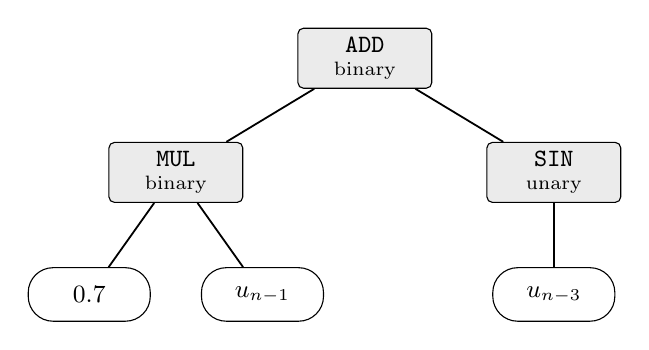
\begin{tikzpicture}[
    operator/.style={
        draw,
        rounded corners=2pt,
        fill=black!8,
        minimum width=1.7cm,
        minimum height=0.72cm,
        align=center,
        font=\small
    },
    leaf/.style={
        draw,
        rounded corners=9pt,
        fill=white,
        minimum width=1.55cm,
        minimum height=0.68cm,
        align=center,
        font=\small
    },
    branch/.style={draw, line width=0.65pt}
]
    \node[operator] (add) at (0,0)
        {\texttt{ADD}\\[-1mm]{\scriptsize binary}};
    \node[operator] (mul) at (-2.4,-1.45)
        {\texttt{MUL}\\[-1mm]{\scriptsize binary}};
    \node[operator] (sin) at (2.4,-1.45)
        {\texttt{SIN}\\[-1mm]{\scriptsize unary}};

    \node[leaf] (constant) at (-3.5,-3.0) {$0.7$};
    \node[leaf] (lagone) at (-1.3,-3.0) {$u_{n-1}$};
    \node[leaf] (lagthree) at (2.4,-3.0) {$u_{n-3}$};

    \draw[branch] (add) -- (mul);
    \draw[branch] (add) -- (sin);
    \draw[branch] (mul) -- (constant);
    \draw[branch] (mul) -- (lagone);
    \draw[branch] (sin) -- (lagthree);
\end{tikzpicture}
\caption{Example unary--binary tree for
$u_n=0.7u_{n-1}+\sin(u_{n-3})$. Binary nodes have two children, the unary
\texttt{SIN} node has one child, and the leaves contain a constant or a lagged
sequence term.}
\label{fig:dascoli-unary-binary-tree}
\end{figure}

Reading Fig.~\ref{fig:dascoli-unary-binary-tree} from the root and recursively
visiting each subtree from left to right produces the prefix representation.
The same tree is serialized in prefix, or Polish, notation, giving a target
such as
\[
    [\texttt{add},\texttt{mul},0.7,u_{n-1},
      \texttt{sin},u_{n-3}].
\]
This representation preserves tree structure without parentheses and allows
the Transformer decoder to generate the recurrence as a token sequence.

\paragraph{How a recovered formula is evaluated.}
Different syntax trees can express the same numerical mechanism. Consequently,
the paper evaluates a predicted recurrence behaviorally: it executes the
predicted and reference formulas from the same initial conditions and checks
the relative error of the next $n_{\mathrm{pred}}$ terms against a tolerance.
This avoids treating an algebraically equivalent expression as wrong merely
because its tokens differ. Beam candidates can likewise be ranked by executing
them and measuring how well they reconstruct the observed sequence.

\paragraph{Contribution to the proposed benchmark.}
This work supplies an expression-first formula sampler for the present thesis:
sample a valid abstract syntax tree, retain that tree as the auditable
mechanism, and execute it to obtain observations. The thesis can extend the
leaf vocabulary with explicit multivariate operators such as
$\operatorname{LAG}(j,\ell)$ and extend the grammar with stochastic
innovations, regime switches, and controlled interaction nodes. Retaining the
sampled tree then supports several references from the same example: its exact
symbolic equation, variable--lag support, signed coefficients when defined,
realized local term values, and generator-based attributions. In the original
study, the tree supervises symbolic-recurrence recovery; in this benchmark, the
same retained mechanism additionally anchors explanation-ground-truth
generation and comparison with forecasting and XAI methods.

\subsubsection{HVAE for Efficient Generation of Mathematical Expressions}

In \emph{Efficient Generator of Mathematical Expressions for Symbolic
Regression}, \citet{meznar2023efficient} address the generation of candidate
equations for symbolic regression. Their central model is a hierarchical
variational autoencoder (HVAE) that represents every expression directly as a
binary tree: internal nodes contain binary operators or unary functions, while
leaves contain variables or constants. The associated EDHiE method searches
the HVAE's continuous latent space for an expression whose evaluated values
fit an observed dataset. This makes the paper relevant to the formula-sampling
stage of the proposed benchmark: a learned prior over trees can concentrate
samples around expression structures found in a selected scientific domain.

\paragraph{Where the training trees come from.}
Before HVAE can sample new expressions, it learns from a corpus of valid trees.
In the experiments, this corpus is produced with probabilistic context-free
grammars and then simplified with SymPy. One reported arithmetic grammar
recursively selects addition or subtraction, multiplication or division, and
parenthesized subexpressions, constants, or variables; a second version also
contains sine and cosine. Consequently, HVAE learns the distribution supplied
by its training corpus rather than beginning from an empty expression space.
For the present thesis, that corpus could instead contain safe discrete-time
mechanisms whose leaves are constants, the current index, and
$\operatorname{LAG}(j,\ell)$ terms.

\paragraph{How HVAE learns a distribution over trees.}
The encoder processes a tree bottom-up. At node $v$, a GRU$_{2\rightarrow1}$
cell combines the symbol stored at $v$ with the representations of its left and
right children. The final root representation is mapped to the mean and
log-variance of a Gaussian latent code. The decoder reverses this direction.
It maps a latent vector to a root state and recursively expands the tree with a
GRU$_{1\rightarrow2}$ cell whose shared parameters are reused at every node.
In the notation of this review, one decoding step is

\begin{equation}
\begin{aligned}
\mathbf z &\sim \mathcal N(\mathbf 0,\mathbf I),
&\mathbf h_{\varnothing}&=\mathbf W_z\mathbf z+\mathbf b_z,\\
\boldsymbol\pi_v
  &=\operatorname{softmax}(\mathbf W_s\mathbf h_v+\mathbf b_s),
&s_v&=\arg\max_s \pi_{v,s},\\
(\mathbf h_{vL},\mathbf h_{vR})
  &=\operatorname{GRU}_{1\rightarrow2}
    (\boldsymbol\pi_v,\mathbf h_v).&&
\end{aligned}
\label{eq:meznar-hvae-decoder}
\end{equation}

The selected symbol determines the tree structure. A binary operator activates
both child states, a unary function activates only the left child, and a
variable or constant terminates that branch. The released decoder selects the
largest softmax probability and, at the configured maximum height, restricts
the choice to leaf symbols.\footnote{Official HVAE implementation:
\url{https://github.com/smeznar/HVAE}; see the recursive decoding and
\texttt{sample\_symbol} routines in \texttt{EDHiE/model.py}.} Thus a latent
draw leads to a complete tree by the following recursion:

\begin{enumerate}
    \item sample $\mathbf z\sim\mathcal N(\mathbf 0,\mathbf I)$ and transform it
    into the root state $\mathbf h_{\varnothing}$;
    \item calculate $\boldsymbol\pi_v$ and choose symbol $s_v$ at the current
    node;
    \item if $a(s_v)=2$, create and decode the left and right child states;
    if $a(s_v)=1$, decode only the left state; if $a(s_v)=0$, close the branch;
    \item repeat the same decoder cell until every branch reaches a leaf;
    \item fit any free constants and execute the resulting expression when it
    is evaluated as a symbolic-regression candidate.
\end{enumerate}

\begin{figure}[H]
\centering
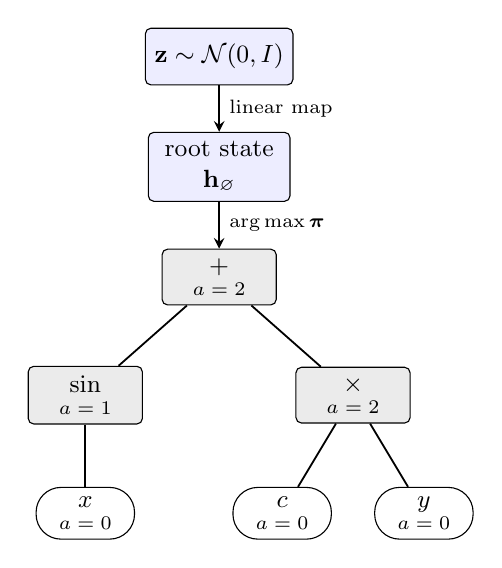
\begin{tikzpicture}[
    state/.style={
        draw,
        rounded corners=2pt,
        fill=blue!7,
        minimum width=1.8cm,
        minimum height=0.72cm,
        align=center,
        font=\small
    },
    operator/.style={
        draw,
        rounded corners=2pt,
        fill=black!8,
        minimum width=1.45cm,
        minimum height=0.68cm,
        align=center,
        font=\small
    },
    leaf/.style={
        draw,
        rounded corners=9pt,
        fill=white,
        minimum width=1.25cm,
        minimum height=0.62cm,
        align=center,
        font=\small
    },
    flow/.style={->,>=stealth,draw,line width=0.7pt},
    branch/.style={draw,line width=0.65pt}
]
    \node[state] (latent) at (0,1.8)
        {$\mathbf z\sim\mathcal N(0,I)$};
    \node[state] (rootstate) at (0,0.4)
        {root state\\$\mathbf h_{\varnothing}$};
    \node[operator] (add) at (0,-1.0)
        {$+$\\[-1mm]{\scriptsize $a=2$}};
    \node[operator] (sin) at (-1.7,-2.5)
        {$\sin$\\[-1mm]{\scriptsize $a=1$}};
    \node[operator] (mul) at (1.7,-2.5)
        {$\times$\\[-1mm]{\scriptsize $a=2$}};
    \node[leaf] (x) at (-1.7,-4.0)
        {$x$\\[-1mm]{\scriptsize $a=0$}};
    \node[leaf] (c) at (0.8,-4.0)
        {$c$\\[-1mm]{\scriptsize $a=0$}};
    \node[leaf] (y) at (2.6,-4.0)
        {$y$\\[-1mm]{\scriptsize $a=0$}};

    \draw[flow] (latent) -- node[right,font=\scriptsize]{linear map}
        (rootstate);
    \draw[flow] (rootstate) -- node[right,font=\scriptsize]{$\arg\max\boldsymbol\pi$}
        (add);
    \draw[branch] (add) -- (sin);
    \draw[branch] (add) -- (mul);
    \draw[branch] (sin) -- (x);
    \draw[branch] (mul) -- (c);
    \draw[branch] (mul) -- (y);
\end{tikzpicture}
\caption{Top-down HVAE decoding of one latent draw into the valid expression
$\sin(x)+c\,y$. Each predicted symbol determines how many descendant states
are decoded: two for a binary operator, one for a unary function, and zero for
a leaf.}
\label{fig:meznar-hvae-sampling}
\end{figure}

The standard sampling method, HVAR, repeats this process for independent
Gaussian latent draws. EDHiE searches the same space more deliberately: its
initial population is sampled from $\mathcal N(\mathbf 0,\mathbf I)$, crossover
forms convex combinations of two parent vectors, and mutation interpolates
between the encoded neighborhood of one expression and the standard Gaussian
prior. Candidate fitness is calculated only after decoding the vector, fitting
its constants, and evaluating the resulting equation on the observations
\citep{meznar2023efficient}.

\paragraph{Efficiency and relevance to the benchmark.}
The experiments report syntactically valid HVAE outputs, substantially lower
reconstruction error with 2,000 training expressions than the sequential VAE
obtains with 12,000, and effective operation in a 32-dimensional latent space.
On the Nguyen benchmark, latent-space random search reconstructs more equations
than the manually specified probabilistic-grammar baseline, while EDHiE adds an
evolutionary search over the learned space. For the proposed benchmark, HVAE
could therefore replace uniform formula sampling with a domain-shaped prior.
Its symbol library would include $\operatorname{LAG}(j,\ell)$, and each decoded
tree would pass numerical-domain, stability, variable-coverage, and recurrence
checks before it generated a time series. The retained decoded tree would then
supply the same structural, coefficient, local-contribution, gradient, and
Shapley references defined elsewhere in this thesis.

\subsubsection{Controllable Neural Symbolic Regression}

\citet{bendinelli2023controllable} introduce Neural Symbolic Regression with
Hypotheses (NSRwH). The method receives both a numerical dataset and a set of
user-supplied hypotheses about the desired equation, then generates candidate
expressions conditioned on both sources. It extends the pretrained neural
symbolic-regression pipeline of NeSymReS \citep{biggio2021neural}: synthetic
expressions are sampled and evaluated to create training pairs, while a
Transformer learns the inverse mapping from the evaluated points back to a
prefix expression. NSRwH adds explicit structural control to this inverse
mapping.

\paragraph{How the synthetic expressions and numerical data are sampled.}
Every training example is a triple $(e,\mathcal D,\mathcal H)$. The first two
elements are constructed as follows \citep{bendinelli2023controllable}.

\begin{enumerate}
    \item Sample a random unary--binary expression-tree shape using the
    procedure of Lample and Charton. The paper restricts depth to
    $1,\ldots,6$, prefix length to at most 20 tokens, and the number of input
    variables to at most five. The released configuration also sets a maximum
    of six operator insertions.

    \item Assign an operator of matching arity to every internal node. The
    reported unary library is
    \[
      \{\sqrt{\cdot},(\cdot)^2,(\cdot)^3,(\cdot)^4,
        (\cdot)^{-1},\log,\exp,\sin,\cos,\arcsin\};
    \]
    the binary library is $\{+,-,\times,\div\}$. Leaves receive variables
    $x_1,\ldots,x_5$ or constant placeholders.

    \item Simplify the expression with SymPy. Sample additive constants
    uniformly on $[-10,10]$ and positive multiplicative constants
    log-uniformly on $[0.05,10]$.

    \item For each active variable, sample the two limits of its support from
    $[-10,10]$, requiring an interval width of at least one. Then sample
    $n\in\{1,\ldots,1000\}$ input points independently within those limits.

    \item Evaluate $e$ at the sampled points to obtain
    $\mathcal D=\{(\mathbf x_i,e(\mathbf x_i))\}_{i=1}^{n}$. Inputs producing
    NaNs or magnitudes above the half-precision limit 65504 are discarded and
    resampled.
\end{enumerate}

The official generator makes the first step more precise. It precomputes the
number of unary--binary trees that can complete each combination of open leaf
positions and remaining operators. At each iteration it uses these counts to
sample (i) which still-empty position receives the next operator and (ii)
whether that operator is unary or binary. It then samples the concrete operator
from configurable weights, opens the required child positions, and eventually
fills all remaining positions with variables. This produces a complete prefix
tree with a controlled operator budget rather than growing branches until an
uncontrolled stopping event.\footnote{Official NSRwH implementation:
\href{https://github.com/SymposiumOrganization/ControllableNeuralSymbolicRegression}
{official NSRwH repository}; see \texttt{dataset/generator.py} and
\texttt{configs/dataset\_configuration.json}.}

\paragraph{How the hypotheses are generated.}
During pretraining, $\mathcal H$ is extracted from the known sampled expression
$e$. At inference, the same fields can be supplied by a scientist as complete,
partial, or uncertain prior knowledge.

\begin{table}[tbp]
\centering
\small
\renewcommand{\arraystretch}{1.08}
\begin{tabular}{@{}p{0.22\textwidth}p{0.70\textwidth}@{}}
\toprule
Hypothesis & Information encoded for the expression decoder \\
\midrule
Complexity & Number of operators, variables, and constants in the expression. \\
Symmetry & Tokens indicating whether selected groups of input variables have
generalized symmetry. \\
Positive branches & Prefix subtrees known to occur in $e$. The complete tree
and trivial one-variable branches are excluded. \\
Negative branches & Prefix subtrees selected from the training distribution
and known to be absent from $e$. \\
Known constants & Numerical constant values paired with pointer tokens that
identify where the decoder may place them. \\
\bottomrule
\end{tabular}
\caption{The five hypothesis families used to condition NSRwH.}
\label{tab:nsrwh-hypotheses}
\end{table}

Positive and negative candidate subtrees are enumerated with depth-first
search. A subtree of prefix length $L_s$ is sampled with weight proportional
to $L_s^{-2}$, so short fragments are presented more often. Parameters
$p_{+}$ and $p_{-}$ control the total number of positive and negative tokens:
sampling continues until their aggregate lengths reach approximately
$p_{+}|e|$ and $p_{-}|e|$, respectively. Masking different hypothesis families
during training teaches one model to operate with many levels of available
prior information.

\paragraph{Architecture and controlled expression decoding.}
NSRwH contains a numerical set encoder, a symbolic hypothesis encoder, and an
autoregressive Transformer decoder. Numerical values first receive a 16-bit
multi-hot representation and an embedding. A set Transformer maps the
unordered input--output points to $\mathbf z_{\mathrm{num}}$. A second set
Transformer maps the hypothesis tokens to $\mathbf z_{\mathrm{hyp}}$. Both
outputs have compatible shape and are combined elementwise:

\begin{equation}
\begin{aligned}
\mathbf z_{\mathrm{num}}&=\operatorname{Enc}_{\mathrm{num}}(\mathcal D),\\
\mathbf z_{\mathrm{hyp}}&=\operatorname{Enc}_{\mathrm{hyp}}(\mathcal H),\\
\mathbf z_{\mathrm{fuse}}&=
    \mathbf z_{\mathrm{num}}+\mathbf z_{\mathrm{hyp}},\\
p_{\phi}(e\mid\mathcal D,\mathcal H)
    &=\operatorname{Dec}_{\phi}(\mathbf z_{\mathrm{fuse}}).
\end{aligned}
\label{eq:nsrwh-fusion}
\end{equation}

The decoder predicts the prefix expression token by token and uses beam search
to retain several candidates. Equation~\eqref{eq:nsrwh-fusion} is the source of
controllability: changing $\mathcal H$ changes the decoder distribution without
retraining the network. Known numerical constants use pointer tokens, avoiding
one vocabulary entry for every possible real number. Remaining constants are
fitted with BFGS, after which candidates are ranked by their numerical fit.

The reported model was trained on 200 million expressions using three NVIDIA
RTX 3090 GPUs for five days with batch size 400. The numerical encoder and
expression decoder each use five layers; the hidden dimension is 512. Training
uses teacher-forced next-token cross-entropy, while inference uses beam search.
The paper separates three evaluation questions: \emph{is satisfied} measures
how often decoded expressions obey the supplied hypothesis; \emph{is correct}
requires numerical agreement at more than 99\% of held-out support points; and
mean $R^2$ measures numerical fit. This distinction prevents an expression that
obeys the requested structure but predicts poorly from being counted as a
successful mechanism recovery.

\begin{figure}[H]
\centering
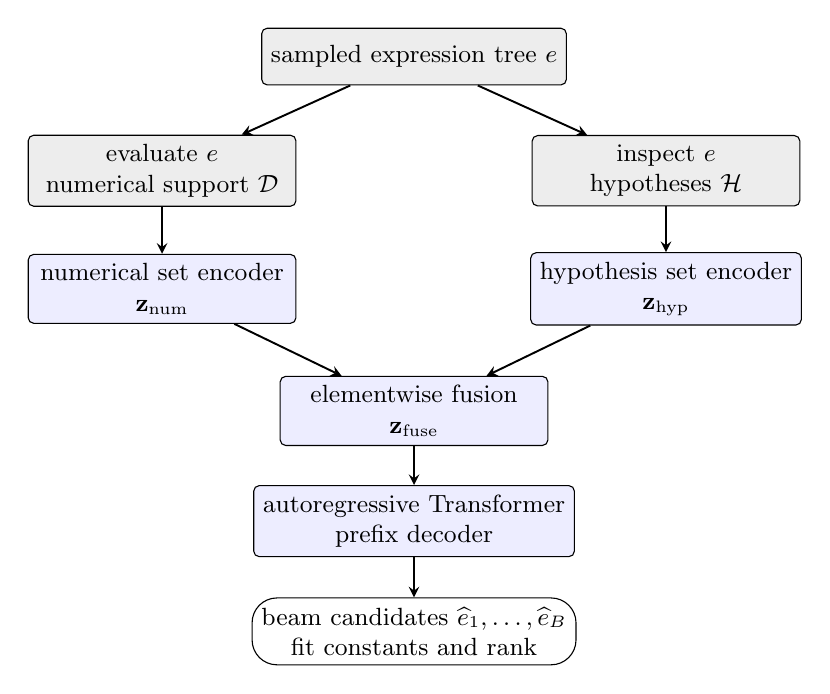
\begin{tikzpicture}[
    block/.style={
        draw,
        rounded corners=2pt,
        fill=blue!7,
        minimum width=3.4cm,
        minimum height=0.72cm,
        align=center,
        font=\small
    },
    source/.style={
        draw,
        rounded corners=2pt,
        fill=black!7,
        minimum width=3.4cm,
        minimum height=0.72cm,
        align=center,
        font=\small
    },
    output/.style={
        draw,
        rounded corners=9pt,
        fill=white,
        minimum width=4.0cm,
        minimum height=0.68cm,
        align=center,
        font=\small
    },
    flow/.style={->,>=stealth,draw,line width=0.7pt}
]
    \node[source] (tree) at (0,3.2)
        {sampled expression tree $e$};
    \node[source] (data) at (-3.2,1.75)
        {evaluate $e$\\numerical support $\mathcal D$};
    \node[source] (hyp) at (3.2,1.75)
        {inspect $e$\\hypotheses $\mathcal H$};
    \node[block] (numenc) at (-3.2,0.25)
        {numerical set encoder\\$\mathbf z_{\mathrm{num}}$};
    \node[block] (hypenc) at (3.2,0.25)
        {hypothesis set encoder\\$\mathbf z_{\mathrm{hyp}}$};
    \node[block] (fuse) at (0,-1.3)
        {elementwise fusion\\$\mathbf z_{\mathrm{fuse}}$};
    \node[block] (decoder) at (0,-2.7)
        {autoregressive Transformer\\prefix decoder};
    \node[output] (candidates) at (0,-4.1)
        {beam candidates $\widehat e_1,\ldots,\widehat e_B$\\
         fit constants and rank};

    \draw[flow] (tree) -- (data);
    \draw[flow] (tree) -- (hyp);
    \draw[flow] (data) -- (numenc);
    \draw[flow] (hyp) -- (hypenc);
    \draw[flow] (numenc) -- (fuse);
    \draw[flow] (hypenc) -- (fuse);
    \draw[flow] (fuse) -- (decoder);
    \draw[flow] (decoder) -- (candidates);
\end{tikzpicture}
\caption{NSRwH training pipeline. The same sampled tree supplies the numerical
observations and the structurally correct hypothesis tokens. At inference, the
two encoder inputs steer a shared prefix-expression decoder.}
\label{fig:nsrwh-pipeline}
\end{figure}

\paragraph{Contribution to the proposed benchmark.}
NSRwH provides a design for controlled mechanism retrieval. The benchmark can
derive $\mathcal H$ automatically from every retained generator tree, then
evaluate recovery under complete, partial, deliberately missing, or partially
incorrect hypotheses. For time series, positive and negative branches can
encode required or forbidden variable--lag subtrees, complexity can control
mechanism size, known constants can expose selected coefficients, and symmetry
can describe exchangeable source variables. The generator remains responsible
for structural, signed, local-contribution, gradient, and Shapley ground truth;
NSRwH supplies a controlled symbolic model whose recovered tree can be compared
with that ground truth.

\subsubsection{ODEFormer: symbolic regression of continuous-time dynamics}

\citet{dascoli2024odeformer} study \emph{dynamical symbolic regression}. The
observations are samples of one continuous-time trajectory,
$\{(t_i,\mathbf x_i)\}_{i=1}^{N}$, and the symbolic target is the vector field
that governs its instantaneous evolution:

\begin{equation}
\dot{\mathbf x}(t)=\mathbf f(\mathbf x(t)),
\qquad
\mathbf f=(f_1,\ldots,f_{D_{\mathrm{ode}}}):
\mathbb R^{D_{\mathrm{ode}}}\rightarrow
\mathbb R^{D_{\mathrm{ode}}}.
\label{eq:odeformer-vector-field}
\end{equation}

This extends the expression-first principle used by D'Ascoli et al.: first
sample a symbolic mechanism and then execute it to generate observations. The
tree representation remains unary--binary and the target remains a prefix
token sequence. The important change is the meaning of execution. A recurrence
tree directly calculates the next discrete sample; an ODE tree calculates
$\dot{\mathbf x}$ at the current state, and a numerical solver repeatedly
evaluates that tree to produce the observed trajectory.

\paragraph{Sampling a symbolic ODE system.}
The system dimension is sampled uniformly up to
$D_{\mathrm{ode}}=6$. One expression tree is generated independently for each
component $f_k$. For every component, ODEFormer performs the following steps
\citep{dascoli2024odeformer}:

\begin{enumerate}
    \item sample between one and five binary operators and construct a random
    binary-tree shape using the same completion-count procedure used in
    Transformer symbolic-regression generators;

    \item assign addition with probability $3/4$ or multiplication with
    probability $1/4$ to each binary node, and assign a state variable
    $x_j$, $j\in\{1,\ldots,D_{\mathrm{ode}}\}$, to each leaf;

    \item sample between zero and three unary insertions. Each insertion places
    one of $\sin(\cdot)$, $(\cdot)^{-1}$, or $(\cdot)^2$ above a selected
    subtree whose depth remains below six;

    \item add signed coefficients to terms and affine transformations inside
    unary arguments. Their absolute values are sampled log-uniformly between
    $0.05$ and $20$;

    \item serialize $f_1,\ldots,f_{D_{\mathrm{ode}}}$ in prefix notation and
    separate consecutive component equations with a dedicated token
    $\texttt{|}$.
\end{enumerate}

Subtraction is represented by addition with a negative coefficient, while
division is represented by multiplication with an inverse. For example, the
tree

\begin{equation}
f_1(\mathbf x)=a x_1+\sin(bx_2)
\quad\longleftrightarrow\quad
[\texttt{add},\texttt{mul},a,x_1,
  \texttt{sin},\texttt{mul},b,x_2]
\label{eq:odeformer-prefix-example}
\end{equation}

uses exactly the same symbolic objects as functional or recurrent symbolic
regression. Its meaning is now $\dot x_1=f_1(\mathbf x)$.

\begin{figure}[H]
\centering
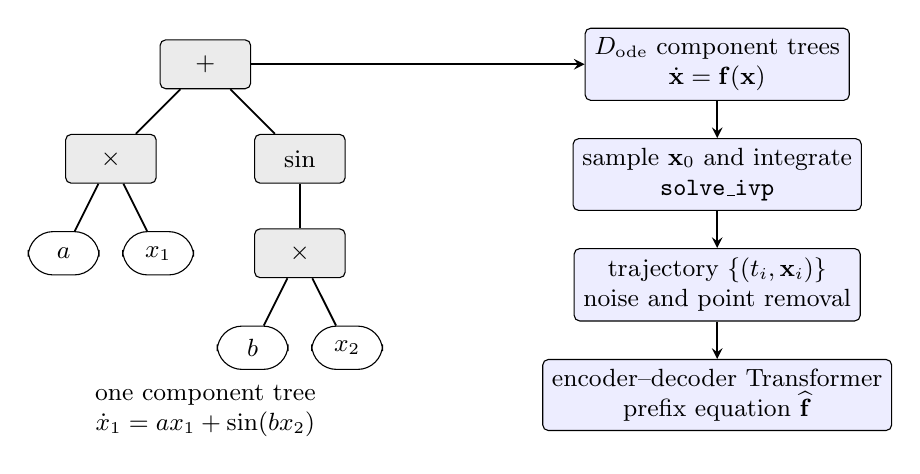
\begin{tikzpicture}[
    operator/.style={draw,rounded corners=2pt,fill=black!8,
        minimum width=1.15cm,minimum height=0.62cm,align=center,font=\small},
    leaf/.style={draw,rounded corners=9pt,fill=white,
        minimum width=0.90cm,minimum height=0.55cm,align=center,font=\small},
    block/.style={draw,rounded corners=2pt,fill=blue!7,
        minimum width=3.15cm,minimum height=0.70cm,align=center,font=\small},
    flow/.style={->,>=stealth,draw,line width=0.7pt},
    branch/.style={draw,line width=0.65pt}
]
    \node[operator] (add) at (-4.4,2.4) {$+$};
    \node[operator] (mul1) at (-5.6,1.2) {$\times$};
    \node[operator] (sin) at (-3.2,1.2) {$\sin$};
    \node[leaf] (a) at (-6.2,0.0) {$a$};
    \node[leaf] (x1) at (-5.0,0.0) {$x_1$};
    \node[operator] (mul2) at (-3.2,0.0) {$\times$};
    \node[leaf] (b) at (-3.8,-1.2) {$b$};
    \node[leaf] (x2) at (-2.6,-1.2) {$x_2$};
    \draw[branch] (add)--(mul1); \draw[branch] (add)--(sin);
    \draw[branch] (mul1)--(a); \draw[branch] (mul1)--(x1);
    \draw[branch] (sin)--(mul2);
    \draw[branch] (mul2)--(b); \draw[branch] (mul2)--(x2);
    \node[font=\small,align=center] at (-4.4,-2.0)
        {one component tree\\$\dot x_1=a x_1+\sin(bx_2)$};

    \node[block] (trees) at (2.1,2.4)
        {$D_{\mathrm{ode}}$ component trees\\$\dot{\mathbf x}=\mathbf f(\mathbf x)$};
    \node[block] (integrate) at (2.1,1.0)
        {sample $\mathbf x_0$ and integrate\\\texttt{solve\_ivp}};
    \node[block] (trajectory) at (2.1,-0.4)
        {trajectory $\{(t_i,\mathbf x_i)\}$\\noise and point removal};
    \node[block] (transformer) at (2.1,-1.8)
        {encoder--decoder Transformer\\prefix equation $\widehat{\mathbf f}$};
    \draw[flow] (add.east) -- (trees.west);
    \draw[flow] (trees)--(integrate);
    \draw[flow] (integrate)--(trajectory);
    \draw[flow] (trajectory)--(transformer);
\end{tikzpicture}
\caption{What remains and what changes in ODEFormer. The symbolic mechanism is
still a unary--binary tree. Numerical integration is inserted between that
tree and the observations because the tree specifies a derivative rather than
the next sample directly.}
\label{fig:odeformer-tree-pipeline}
\end{figure}

\paragraph{From an equation to a training trajectory.}
After sampling $\mathbf f$, the generator draws
$\mathbf x_0\sim\mathcal N(\mathbf 0,\mathbf I)$ and integrates
Equation~\eqref{eq:odeformer-vector-field} from $t=1$ to $t=10$. The number of
stored points $N$ is sampled uniformly from 50 to 200. The implementation uses
SciPy's \texttt{solve\_ivp}, whose default method is adaptive RK45. Failed
integrations and trajectories with $|x_j|>10^2$ are discarded. When every
component becomes nearly constant during the final quarter of the interval,
the example is discarded with probability $0.9$ so that fixed-point solutions
do not dominate the training distribution.

Two corruptions make the observations resemble measurements. A noise scale
$\sigma\sim\mathcal U(0,0.1)$ produces multiplicative Gaussian noise,

\begin{equation}
x_j(t_i)\leftarrow(1+\xi_{i,j})x_j(t_i),
\qquad \xi_{i,j}\sim\mathcal N(0,\sigma^2),
\label{eq:odeformer-noise}
\end{equation}

and a sampled ratio $\rho\sim\mathcal U(0,0.5)$ removes that fraction of time
points uniformly. Consequently, a training pair contains a noisy, irregularly
sampled trajectory as input and the exact prefix representation of the sampled
vector field as target. The formula is retained before integration, so it is
available as mechanism ground truth.

\paragraph{Architecture and inference.}
ODEFormer uses an encoder--decoder Transformer with 86 million parameters, 16
attention heads, and embedding dimension 512. The encoder has four layers and
the decoder has 16. Each timestamp and state value is rounded to four
significant digits and represented by three tokens: sign, mantissa, and
exponent. A feed-forward embedder combines the tokens belonging to one observed
point. Since time is included explicitly in every point, the numerical encoder
uses the timestamps instead of positional embeddings.

The decoder generates the component equations autoregressively in prefix
notation. Beam sampling produces candidate systems; the reported default uses
beam size 50 and temperature 0.1. Every candidate is integrated from the
observed initial condition, and the equation with the highest reconstruction
$R^2$ is selected. An optional BFGS step refines numerical constants. The
complete implementation is released by the authors.\footnote{Official
ODEFormer implementation: \url{https://github.com/sdascoli/odeformer}.}

\paragraph{How mechanism recovery is evaluated.}
The paper distinguishes two trajectory-level tests:

\begin{itemize}
    \item \emph{reconstruction}: integrate $\widehat{\mathbf f}$ from the same
    initial condition and over the same interval used to produce the observed
    trajectory;
    \item \emph{generalization}: integrate $\mathbf f$ and
    $\widehat{\mathbf f}$ from a new initial condition, then compare their
    trajectories over the same time interval.
\end{itemize}

The principal accuracy statistic is the percentage of systems for which the
trajectory $R^2$ exceeds $0.9$. The authors additionally report expression
complexity, defined as the total number of operators, variables, and constants,
and inference time. Generalization is the stronger mechanism-recovery test: two
equations may follow one observed path while generating different dynamics in
other parts of the state space. This also explains why recovering an ODE from
one trajectory is an identifiability problem rather than only a forecasting
problem.

\paragraph{What the recovered ODE explains.}
An explicit ODE gives a global, mechanistic description of the instantaneous
dynamics. For example, the occurrence of $x_j$ in $f_k$ states that variable
$j$ directly participates in the rate of change of variable $k$. This yields a
structural reference

\begin{equation}
M^{\mathrm{GT,ODE}}_{k,j}
=\mathbb I[x_j\text{ occurs in the sampled tree for }f_k].
\label{eq:odeformer-structural-gt}
\end{equation}

A local derivative-level influence can also be calculated from the Jacobian,

\begin{equation}
J_{k,j}(t)=
\left.\frac{\partial f_k(\mathbf x)}{\partial x_j}
\right|_{\mathbf x=\mathbf x(t)}.
\label{eq:odeformer-jacobian}
\end{equation}

These quantities explain which variables govern the \emph{instantaneous rate
of change}. Explaining a finite-horizon state
$\Phi_{\mathbf f}(\Delta;\mathbf x_0)$ requires propagating influence through
the integration. One principled reference is the flow sensitivity

\begin{equation}
\mathbf S(\Delta)=
\frac{\partial\Phi_{\mathbf f}(\Delta;\mathbf x_0)}{\partial\mathbf x_0},
\qquad
\dot{\mathbf S}(t)=
\mathbf J_{\mathbf f}(\mathbf x(t))\mathbf S(t),
\quad \mathbf S(0)=\mathbf I.
\label{eq:odeformer-flow-sensitivity}
\end{equation}

Equations~\eqref{eq:odeformer-structural-gt}--
\eqref{eq:odeformer-flow-sensitivity} are a benchmark interpretation proposed
for this thesis. ODEFormer evaluates reconstructed and generalized trajectories
instead. The distinction resolves the apparent loss of explainability: the
symbolic ODE makes the governing law explicit, while a contribution to a
particular future state additionally depends on the initial condition, the
visited trajectory, interactions, and the chosen horizon.

\paragraph{Position in the proposed research.}
ODEFormer provides a useful advanced extension and a methodological bridge to
continuous-time system identification. The November benchmark can keep its
core around discrete-time recurrences, where a sampled tree directly generates
the next observation and all variable--lag references are immediate. A later
continuous-time module can reuse the same expression-tree interface while
adding initial-condition sampling, numerical integration, solver-failure
filters, and flow-based explanation references. This staging preserves the
main software design while separating the additional numerical and
identifiability challenges of ODE discovery.

\paragraph{Differences among the four approaches in Section~1.2.}
D'Ascoli et al. directly sample a discrete lagged recurrence, execute it to
produce a sequence, and train a Transformer to recover the recurrence from that
sequence. Me\v{z}nar et al. learn an unconditional continuous prior over general
expression trees and search that latent space for equations fitting numerical
data. Bendinelli et al. retain an explicit random-tree prior for pretraining and
learn the conditional inverse map
$p_{\phi}(e\mid\mathcal D,\mathcal H)$, allowing hypotheses to steer which
equation is recovered. NSRwH is therefore a direct extension of the NeSymReS
family and contributes controlled recovery; D'Ascoli's construction supplies
the discrete temporal-generator role. ODEFormer retains random unary--binary
trees and prefix decoding, but interprets each tree as one component of a
continuous-time vector field and uses numerical integration to connect the
equation with observations. For this thesis, the four contributions compose
naturally: D'Ascoli supplies the lagged grammar and executable recurrence, HVAE
offers an optional learned prior over plausible recurrence trees, NSRwH supplies
a retriever that can be tested with different amounts and qualities of known
mechanism information, and ODEFormer supplies the continuous-time extension in
which evaluation must include trajectory reconstruction and generalization.

\subsection{Synthetic Priors for Time-Series Foundation Models}

This subsection examines a second use of synthetic time series: constructing a
large pretraining distribution for a forecasting foundation model. The central
object in these works is a \emph{prior over possible series}. Sampling many
independent mechanisms and trajectories exposes one model to a wider range of
trends, seasonalities, correlations, regime changes, and noise processes than
is available in a single real dataset. This objective complements the
explanation benchmarks in Section~1.1: the same generator can provide training
diversity, while a benchmark additionally retains the sampled mechanism and
derives an explicit reference explanation from it.

\subsubsection{KernelSynth and its role in Chronos-2}

\paragraph{Provenance and role.}
KernelSynth was introduced with the original Chronos model by
\citet{ansari2024chronos}. Chronos-2 subsequently uses KernelSynth as one of
four base univariate generators---AR, ETS, TSI, and KernelSynth---before
imposing multivariate structure through additional transformations
\citep{ansari2025chronos2}. Thus, KernelSynth supplies elementary stochastic
trajectories; the Chronos-2 data pipeline supplies the cross-series structure
needed for multivariate and covariate-informed tasks.

\paragraph{How KernelSynth generates one series.}
KernelSynth reverses the compositional-kernel-search idea. Instead of observing
a series and searching for a Gaussian-process kernel that describes it, the
method first samples a composite kernel and then draws a function from the
corresponding Gaussian-process prior. Let $\mathcal K$ be the kernel bank and
let $J_K=5$ be the maximum number of kernels in one composition. The procedure
is

\begin{equation}
\begin{aligned}
R_K &\sim \mathcal U\{1,\ldots,J_K\},\\
\kappa_1,\ldots,\kappa_{R_K}
    &\overset{\mathrm{i.i.d.}}{\sim}\mathcal K,\\
\kappa_\star
    &=(((\kappa_1\circ_2\kappa_2)\circ_3\kappa_3)\cdots)
      \circ_{R_K}\kappa_{R_K},
      \qquad \circ_r\sim\mathcal U\{+,\times\},\\
x_{1:T_{\mathrm{syn}}}
    &\sim \operatorname{GP}(0,\kappa_\star),
    \qquad T_{\mathrm{syn}}=1024.
\end{aligned}
\label{eq:kernelsynth}
\end{equation}

The final line means that the implementation evaluates $\kappa_\star$ on the
chosen time grid to obtain a covariance matrix $\mathbf K_\star$, then samples
the complete vector
$\mathbf x\sim\mathcal N(\mathbf 0,\mathbf K_\star)$. Every draw is therefore
a different trajectory even when the same composite kernel is reused. The
kernel bank in the paper and released implementation is summarized in
Table~\ref{tab:kernelsynth-bank}.

\begin{table}[H]
\centering
\small
\renewcommand{\arraystretch}{1.08}
\begin{tabular}{@{}p{0.19\textwidth}p{0.36\textwidth}p{0.36\textwidth}@{}}
\toprule
Kernel family & Temporal behavior represented & Values used in the bank \\
\midrule
Constant & Shared level covariance & $C=1$ \\
White noise & Independent short-scale variation & noise level $0.1$ or $1$ \\
Linear & Globally varying trend-like functions & offset scale $0$, $1$, or $10$ \\
RBF & Smooth local variation & length scale $0.1$, $1$, or $10$ \\
Rational quadratic & Variation over a mixture of smoothness scales &
shape $0.1$, $1$, or $10$ \\
Periodic & Repeating patterns over common temporal frequencies &
hourly-, daily-, weekly-, monthly-, quarterly-, and yearly-inspired periods \\
\bottomrule
\end{tabular}
\caption{Basis-kernel families used by KernelSynth. The released code stores
several parameterized instances of each family in $\mathcal K$, so sampling is
over kernel type and parameterization.}
\label{tab:kernelsynth-bank}
\end{table}

Kernel addition and multiplication have distinct meanings. If
$\kappa_\star=\kappa_a+\kappa_b$, a GP draw can be interpreted as the sum of
independent functions with the two covariance structures. A linear-plus-
periodic composition can consequently express trend-like and seasonal
variation together. If
$\kappa_\star=\kappa_a\kappa_b$, similarity must be supported by both factors;
an RBF-times-periodic composition produces locally periodic behavior whose
correlation weakens with temporal distance. Repeated random compositions
therefore create a broad stochastic prior from a small kernel vocabulary.

\paragraph{How Chronos-2 constructs multivariate training tasks.}
Chronos-2 uses separate synthetic mechanisms at two levels
\citep{ansari2025chronos2}. Its univariate corpus is enlarged with TSI, which
randomly combines trend, seasonality, and irregularity components, and TCM,
which samples temporal causal graphs and generates series autoregressively.
For multivariate and covariate-informed pretraining, the data are synthetic.
A \emph{multivariatizer} first samples several base series from AR, ETS, TSI,
or KernelSynth and then introduces one of two dependency classes:

\begin{itemize}
    \item a contemporaneous multivariatizer jointly transforms several series,
    linearly or nonlinearly, at each time step. This creates instantaneous
    cross-series dependence;
    \item a sequential multivariatizer introduces dependence across different
    time steps, including lead--lag effects and cointegration-like behavior.
\end{itemize}

The resulting channels are used either as joint targets or are divided into
targets, past-only covariates, and known-future covariates. This construction
is important for interpreting the phrase ``KernelSynth in Chronos-2'':
KernelSynth creates a base univariate GP draw, while the multivariatizer is the
stage that creates the multivariate forecasting problem. The Chronos-2 paper
specifies these two classes and their purpose; the exact sampled transformation
families and parameter distributions remain outside the report's description.

\paragraph{Generation implementation and computational scaling.}
The official Chronos KernelSynth script exposes the generation as an
embarrassingly parallel offline job. Independent series are dispatched over
all available CPU workers with \texttt{joblib.Parallel}, configured with
\texttt{n\_jobs=-1}, and the
result is written to an Apache Arrow file with LZ4 compression. A composite
kernel is evaluated as a dense $T_{\mathrm{syn}}\times T_{\mathrm{syn}}$
covariance matrix. Exact GP sampling therefore retains cubic factorization
cost in $T_{\mathrm{syn}}$ and quadratic memory, while process-level parallelism
raises corpus throughput by generating different series concurrently. The
released script also defines an eigendecomposition-based sampling alternative;
its main generation path uses scikit-learn's GP sampler. This implementation
detail matters for the proposed benchmark: GP examples can be generated in
parallel, but long trajectories require either bounded length, approximate GP
sampling, structured kernels, or a different procedural generator.

\paragraph{Architecture that consumes the synthetic corpus efficiently.}
Chronos-2 is a 120M-parameter encoder-only Transformer derived from the T5
encoder \citep{ansari2025chronos2}. Each target or covariate dimension is
standardized from its observed context and transformed with $\operatorname{asinh}$
to compress extreme values while preserving sign. The normalized values, a
relative-time feature, and an observed/missing mask are divided into
non-overlapping patches of length $P_{\mathrm{patch}}$ and mapped by a residual
network into $D_{\mathrm{model}}$-dimensional tokens. The Transformer then
alternates:

\begin{enumerate}
    \item \emph{time attention}, which attends across patches belonging to the
    same series and uses rotary positional embeddings; and
    \item \emph{group attention}, which attends across related series at the
    same patch index, using group IDs to isolate independent forecasting tasks.
\end{enumerate}

A residual quantile head maps all requested future-patch embeddings directly
to 21 quantiles for every target and forecast step. Direct multi-patch output
avoids token-by-token trajectory sampling. Training first uses contexts up to
2048 observations and then extends them to 8192 while increasing the number of
output patches. The report measures approximately 300 series per second on one
NVIDIA A10G for a batch of 1024 series with context 2048 and horizon 64. These
designs make the \emph{forecasting model} efficient; CPU-parallel GP sampling
is the separate mechanism that constructs the original KernelSynth corpus.

\paragraph{Explanation information available from KernelSynth.}
The sampled composite kernel $\kappa_\star$ is an exact record of the stochastic
mechanism. For an observed context $\mathbf x_C$, the GP conditional-mean
forecast at horizon $h$ is

\begin{equation}
g_h(\mathbf x_C;\kappa_\star)
=\mu_{h\mid C}
=\mathbf k_{hC}
  (\mathbf K_{CC}+\sigma_n^2\mathbf I)^{-1}\mathbf x_C,
\label{eq:gp-conditional-mean}
\end{equation}

so its exact input gradient is the horizon-specific row vector

\begin{equation}
\nabla_{\mathbf x_C}g_h
=\mathbf k_{hC}
 (\mathbf K_{CC}+\sigma_n^2\mathbf I)^{-1}.
\label{eq:gp-gradient}
\end{equation}

Equations~\eqref{eq:gp-conditional-mean}--\eqref{eq:gp-gradient} show how a
KernelSynth variant could enter this thesis as a dense stochastic benchmark:
the kernel composition is the mechanism ground truth, while the conditional
mean supplies an executable forecasting function and an exact gradient
reference. The future GP draw additionally contains conditional stochastic
variation, which belongs to irreducible forecast uncertainty rather than to a
deterministic input contribution.

\subsubsection{TempoPFN synthetic prior used by Toto 2.0}

\paragraph{Terminological distinction.}
Two similarly named works must be separated. \emph{TempoPFN}, by
\citet{moroshan2025tempopfn}, is the synthetic-data method cited and used by
Toto 2.0 \citep{khwaja2026toto2}. \emph{TimePFN}, by
\citet{taga2025timepfn}, is a different multivariate forecasting model based on
LMC-Synth; it is analyzed in the next subsection. Toto 2.0 consumes data from
the TempoPFN prior, rather than the TimePFN/LMC-Synth corpus.

\paragraph{How the TempoPFN prior generates series.}
TempoPFN defines a portfolio of complementary generator families rather than
one equation family \citep{moroshan2025tempopfn}. Adapted generators include
ForecastPFN component compositions, KernelSynth, a broader GP prior, and
CauKer structural causal models. New procedural families add sawtooth waves,
piecewise-constant steps, anomaly and spike processes, configurable sine
mixtures, and audio-inspired stochastic rhythms, financial volatility,
network traffic, and multiscale fractal signals. Its most structured stochastic
generator is a regime-switching, time-inhomogeneous Ornstein--Uhlenbeck process,

\begin{equation}
 d y_t
 =\theta(t,r_t)\bigl(\mu(t,r_t)-y_t\bigr)\,dt
  +\sigma(t,r_t)\,dW_t,
\label{eq:tempopfn-ou}
\end{equation}

where the latent regime $r_t\in\{0,1\}$ follows a Markov chain. The mean-
reversion speed, time-varying mean, and volatility can change between regimes
and evolve through polynomial, sinusoidal, logistic, or piecewise-linear
trends. Seasonal effects can modify the mean and volatility, and fractional
Brownian motion can replace $W_t$ to introduce long memory.

After a base trajectory is generated, an offline augmentation cascade expands
the prior. It optionally normalizes the source, applies an early convex
TS-Mixup, samples transformations from invariance, structure, seasonality,
signal-processing, discrete-effect, and measurement-artifact categories,
optionally applies random 1D convolution filters, performs a late TS-Mixup,
and finishes with scaling and low-amplitude noise. Examples include time
reversal, sign inversion, change points, shocks with exponential recovery,
calendar effects, amplitude modulation, differentiation or integration,
censoring, quantization, and resampling artifacts. An online stage injects
missing-value patterns. Consequently, one stored trajectory may combine a
sampled base mechanism with several independently recorded transformations.

\paragraph{High-throughput data construction.}
TempoPFN reports a corpus of approximately 10 million series with lengths up to
2048. Most procedural generators run on CPU, while neural generators such as
CauKer use a GPU. On the authors' dual 32-core AMD EPYC system, throughput for
length-2048 series ranges from $0.32$ series/s for exact KernelSynth and $0.66$
for CauKer to more than $100$ series/s for step, sine, anomaly, spike, and
sawtooth generators. This heterogeneous architecture is deliberate: expensive
GP/causal priors contribute structural richness, while inexpensive procedural
priors supply volume. During training, the loader samples a total length from
$\{128,256,512,1024,1536,2048\}$, favors length 2048, shortens by cutting or
subsampling, and then samples a history--future split. Mixed batches therefore
cover several mechanisms, context lengths, and forecast horizons.

\paragraph{How Toto 2.0 uses this prior.}
The Toto 2.0 report states that its base models are pretrained on 42.5\%
Datadog observability data and 57.5\% TempoPFN synthetic data
\citep{khwaja2026toto2}. The three larger models see 5.04 trillion points, of
which 2.90 trillion are synthetic; the 4M- and 22M-parameter models see 3.40
trillion points with the same proportions. The report identifies the
TempoPFN method and its coverage of nonstationary trends, abrupt change points,
and long-range dependencies. It reports the final mixture rather than an
itemized count for each TempoPFN generator inside the Toto corpus.

Toto 2.0 uses a decoder-only patched Transformer with patch size
$P_{\mathrm{patch}}=32$. Transformer blocks alternate causal attention along
time with full attention across variates. Contiguous patch masking replaces
autoregressive patch generation: during training, the model reconstructs
random contiguous masked spans; during inference, mask tokens occupy the
complete future horizon and the Transformer predicts that horizon in one
forward pass. A block-decoding mode remains available for very long horizons.
The output head predicts nine quantiles and is trained with pinball loss.

Three engineering choices support large-scale training. First, robust causal
$\operatorname{asinh}$ normalization controls the extreme scales and spikes
found in observability metrics. Second, NorMuon optimizes internal matrix
parameters while AdamW handles projections, biases, and normalization
parameters. Third, unit-scaled maximal-update parametrization (u-$\mu$P) lets
the authors tune a 10M-parameter proxy and transfer its learning configuration
to 4M, 22M, 313M, 1B, and 2.5B variants. Their released
\texttt{dd\_unit\_scaling} layer preserves this parametrization through
\texttt{torch.compile}, FSDP2 sharding, and data/tensor parallelism. All model
sizes train with 4096-step contexts, 32 variates per sample, and global batch
size 64. The generator portfolio provides data diversity; patch masking,
alternating attention, u-$\mu$P, and distributed sharding provide model-
training scale.

\paragraph{Explanation information available from the TempoPFN pipeline.}
The generator identity, sampled parameters, regime path, and augmentation
sequence can form a hierarchical mechanism record. For example,
Eq.~\eqref{eq:tempopfn-ou} supplies regime- and time-dependent drift and
diffusion parameters, while a step generator supplies exact change-point
locations. Their current use in Toto 2.0 is forecasting pretraining. For the
present thesis, retaining this metadata would permit evaluation by mechanism
family and controlled difficulty, whereas local gradient or Shapley ground
truth would be calculated from an explicitly selected executable forecasting
functional, such as the conditional mean of the sampled process.

\subsubsection{TimePFN and LMC-Synth as a related multivariate design}

\paragraph{LMC-Synth generation.}
TimePFN constructs cross-channel structure with a linear model of
coregionalization \citep{taga2025timepfn}. It first samples
$N_{\mathrm{lat}}$ from a clipped Weibull distribution. Each latent function
$z_a(t)$ is an independent KernelSynth draw with its own randomly composed GP
kernel. For each observed channel $j$, a Dirichlet vector supplies nonnegative
weights that sum to one:

\begin{equation}
\begin{aligned}
N_{\mathrm{lat}}
    &\sim \operatorname{clip}
      \bigl(\operatorname{Weibull}(\beta,\lambda),m,N\bigr),\\
z_a(t)&\sim\operatorname{KernelSynth}(J_K,T_{\mathrm{syn}}),
      \qquad a=1,\ldots,N_{\mathrm{lat}},\\
(\lambda_{j,1},\ldots,\lambda_{j,N_{\mathrm{lat}}})
    &\sim\operatorname{Dirichlet}(d\mathbf 1),\\
x_j(t)&=\sum_{a=1}^{N_{\mathrm{lat}}}\lambda_{j,a}z_a(t),
      \qquad j=1,\ldots,N.
\end{aligned}
\label{eq:lmc-synth}
\end{equation}

Channels become correlated when they reuse latent functions. Small Dirichlet
concentration produces channel-specific mixtures; larger concentration makes
the mixtures more uniform. The authors also generate an independent-channel
case, $N_{\mathrm{lat}}=N$ and $x_j(t)=z_j(t)$, so the training distribution
covers examples both with and without useful cross-channel dependence.

The reported corpus contains 15,000 synthetic datasets, each with length 1024
and 160 channels. Sliding windows of length 192 are split into 96 context and
96 forecast steps, yielding approximately 1.5 million multivariate training
examples. Independent-channel examples amount to approximately 25\% of the
correlated corpus. Training begins with independent channels and later
introduces correlated mixtures, forming a curriculum from univariate pattern
recognition to cross-channel inference. Multiplicative Gaussian noise with
mean 1 and standard deviation 0.1 regularizes the examples.

\paragraph{Generation and model architecture.}
The released LMC-Synth implementation parallelizes independent multivariate
datasets over all CPU cores with \texttt{joblib}, uses eigendecomposition for
GP sampling, performs the latent-to-channel mixture as a matrix product, and
writes compressed Arrow data. The TimePFN model then processes these data in
four stages:

\begin{enumerate}
    \item each standardized channel passes through shared 1D convolutions and
    magnitude max pooling; nine filtered rows are concatenated with the
    original channel;
    \item overlapping patches of length 16 and stride 8 are flattened and
    mapped to 256-dimensional token embeddings;
    \item two-dimensional sinusoidal encodings identify both time and channel,
    and all channel tokens enter the same eight-layer Transformer encoder, so
    attention performs channel mixing;
    \item a shared two-layer feedforward head maps each reconstructed channel
    representation directly to the 96-step forecast.
\end{enumerate}

The released configuration has approximately 8.5M parameters, accepts a
variable number of channels, and fixes context and prediction lengths to 96.
The paper reports about ten hours of pretraining on one NVIDIA L40S GPU; a
32-core CPU and 128GB RAM support synthetic-data preparation. This is a
compact prior-data-fitted network: many mechanism samples are generated
offline, and one model amortizes forecasting over that prior.

\paragraph{Relevance to the proposed benchmark.}
LMC-Synth retains both the composite kernel of every latent process and the
mixing matrix $[\lambda_{j,a}]$. These objects provide exact ground truth for
latent sharing and covariance between channels. GP dependence is generally
dense over time, so its native reference is a dense temporal covariance rather
than a sparse variable--lag mask. Applying the conditional-mean construction in
Eq.~\eqref{eq:gp-conditional-mean} to the block multivariate covariance would,
however, produce a known horizon--source--time forecasting function and its
exact Jacobian. LMC-Synth is therefore a useful stochastic complement to the
thesis's sparse recurrence generators.

\subsubsection{SymTime and the \texorpdfstring{S$^2$}{S2}Generator
series--symbol prior}

\paragraph{Purpose and position in this review.}
\citet{wang2025symtime} introduce S$^2$Generator to produce paired symbolic
expressions and multivariate time series at the scale required to pretrain
SymTime. The paper belongs in this subsection because its learned output is a
general-purpose time-series representation for downstream analysis. The
symbolic expression acts as a second, semantically aligned view during
pretraining. This differs from the symbolic-regression methods in
Section~1.2, whose learned output is the equation itself.

\paragraph{The complete generated object.}
S$^2$Generator first samples a vector-valued algebraic map
$\mathbf f_{\mathrm{S^2}}:\mathbb R^{M_{\mathrm{S^2}}}\rightarrow
\mathbb R^{N_{\mathrm{S^2}}}$ and then samples the input trajectories to which
that map is applied. In the common notation of Table~\ref{tab:notation}, one
example is

\begin{equation}
\begin{aligned}
x_{j,1:T_{\mathrm{S^2}}}
  &=G_{X,j}(\boldsymbol\eta_j;\boldsymbol\theta_j),
  &&j=1,\ldots,M_{\mathrm{S^2}},\\
y_{i,t}
  &=f_i(x_{1,t},\ldots,x_{M_{\mathrm{S^2}},t}),
  &&i=1,\ldots,N_{\mathrm{S^2}},\quad
    t=1,\ldots,T_{\mathrm{S^2}}.
\end{aligned}
\label{eq:s2-complete-generator}
\end{equation}

Here $G_{X,j}$ denotes the sampled stochastic process for input channel $j$,
$\boldsymbol\theta_j$ its parameters, and $\boldsymbol\eta_j$ its realized
random innovations. The full series generator is consequently the composition
$\mathbf g_{\mathrm{S^2}}=\mathbf f_{\mathrm{S^2}}\circ\mathbf G_X$.
This separation is essential: $\mathbf f_{\mathrm{S^2}}$ describes which
current input variables are algebraically transformed into each current
output, whereas $\mathbf G_X$ supplies the temporal behavior of those inputs.

\paragraph{How the expression trees are sampled.}
The generator exhaustively traverses
$M_{\mathrm{S^2}}\in\{1,\ldots,6\}$ and
$N_{\mathrm{S^2}}\in\{1,\ldots,12\}$ rather than randomly favoring some
input--output dimensions. It samples one separate tree $f_i$ for every output
channel and applies the following construction \citep{wang2025symtime}:

\begin{enumerate}
    \item draw the number of binary nodes
    $b\sim\mathcal U\{b_{\min},\ldots,b_{\max}\}$ and label them uniformly
    from $\{+,-,\times\}$;

    \item combine those nodes into a full binary-tree skeleton. The released
    implementation uses the same open-slot/completion-count sampler found in
    the Transformer symbolic-regression generator family: a binary node
    consumes one open position and creates two, and the next insertion
    position is sampled from the number of valid completions;

    \item choose $m\sim\mathcal U\{1,\ldots,M_{\mathrm{S^2}}\}$ input
    variables for leaves and add random constants to the remaining leaf
    positions needed to complete the tree;

    \item draw $u\sim\mathcal U\{u_{\min},\ldots,u_{\max}\}$ and insert unary
    nodes at random valid positions. The library is
    $\{\operatorname{inv},|\cdot|,(\cdot)^2,(\cdot)^3,\sqrt{\cdot},
    \sin,\cos,\tan,\arctan,\log,\exp\}$;

    \item apply random affine transformations $z\mapsto az+b$ to selected
    variable leaves and unary outputs, increasing coefficient and offset
    diversity without changing the sampled topology.
\end{enumerate}

For example, the tree in Figure~\ref{fig:s2-tree-and-series} represents
$f_i(\mathbf x)=\sin(x_1)+x_2x_3$. Its binary skeleton has a sum at the root
and a product in the right branch; the sine is inserted afterward as a unary
node. The actual generator may wrap these nodes in the sampled affine
transformations.

\begin{figure}[H]
\centering
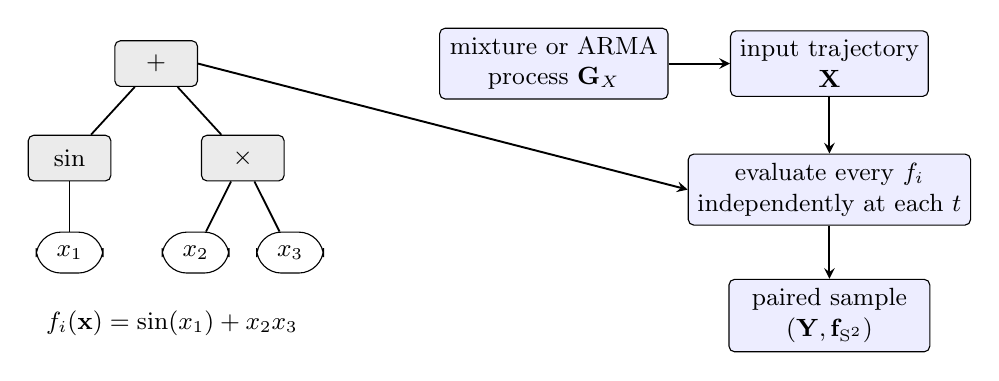
\begin{tikzpicture}[
    operator/.style={draw,rounded corners=2pt,fill=black!8,
        minimum width=1.05cm,minimum height=0.58cm,align=center,font=\small},
    leaf/.style={draw,rounded corners=9pt,fill=white,
        minimum width=0.85cm,minimum height=0.52cm,align=center,font=\small},
    block/.style={draw,rounded corners=2pt,fill=blue!7,
        minimum width=2.55cm,minimum height=0.72cm,align=center,font=\small},
    flow/.style={->,>=stealth,draw,line width=0.7pt},
    branch/.style={draw,line width=0.65pt}
]
    \node[operator] (add) at (-5.4,2.35) {$+$};
    \node[operator] (sin) at (-6.5,1.15) {$\sin$};
    \node[operator] (mul) at (-4.3,1.15) {$\times$};
    \node[leaf] (x1) at (-6.5,-0.05) {$x_1$};
    \node[leaf] (x2) at (-4.9,-0.05) {$x_2$};
    \node[leaf] (x3) at (-3.7,-0.05) {$x_3$};
    \draw[branch] (add)--(sin); \draw[branch] (add)--(mul);
    \draw[branch] (sin)--(x1);
    \draw[branch] (mul)--(x2); \draw[branch] (mul)--(x3);
    \node[font=\small,align=center] at (-5.2,-0.95)
        {$f_i(\mathbf x)=\sin(x_1)+x_2x_3$};

    \node[block,minimum width=2.9cm] (input) at (-0.35,2.35)
        {mixture or ARMA\\process $\mathbf G_X$};
    \node[block,minimum width=2.35cm] (X) at (3.15,2.35)
        {input trajectory\\$\mathbf X$};
    \node[block,minimum width=3.2cm] (f) at (3.15,0.75)
        {evaluate every $f_i$\\independently at each $t$};
    \node[block] (pair) at (3.15,-0.85)
        {paired sample\\$(\mathbf Y,\mathbf f_{\mathrm{S^2}})$};
    \draw[flow] (input)--(X);
    \draw[flow] (X)--(f);
    \draw[flow] (add.east) -- (f.west);
    \draw[flow] (f)--(pair);
\end{tikzpicture}
\caption{S$^2$Generator separates the sampled symbolic transformation from
the process that supplies its temporal inputs. The displayed tree acts on one
aligned input vector $\mathbf x_t$ at a time; mixture or ARMA sampling creates
the trajectory across $t$.}
\label{fig:s2-tree-and-series}
\end{figure}

\paragraph{How temporal inputs and outputs are produced.}
Every input channel is drawn either from a random finite mixture of Gaussian
or uniform distributions, or from a random-parameter ARMA$(p,q)$ process. In
the latter branch, the common notation gives

\begin{equation}
x_{j,t}=\sum_{r=1}^{p}a_{j,r}x_{j,t-r}
          +\eta_{j,t}
          -\sum_{s=1}^{q}\vartheta_{j,s}\eta_{j,t-s}.
\label{eq:s2-arma-input}
\end{equation}

The orders and coefficients are sampled within the bounds reported by the
paper, with constraints intended to favor stationary AR dynamics. Mixture
inputs provide varied marginal distributions; ARMA inputs additionally carry
serial dependence. Each channel of $\mathbf X$ is standardized, all trees are
evaluated pointwise according to Equation~\eqref{eq:s2-complete-generator},
and samples outside an operator's valid domain or with
$|y_{i,t}|>10^4$ are rejected. The released corpus contains 40 million
series--symbol pairs with a cumulative sequence length of 50 billion. For
fixed tree size, channel counts, mixture size, and ARMA orders, the authors'
analysis and timing experiment show generation cost approximately linear in
$T_{\mathrm{S^2}}$. Oversized random trees narrow valid domains and lower the
acceptance rate, which motivates the paper's bounded operator library.

\paragraph{How SymTime uses the pair.}
The time-series branch is a six-layer Transformer trained to reconstruct
masked non-overlapping patches. The symbolic branch is a six-layer DistilBERT
trained with masked-language modeling. Bidirectional series--symbol contrastive
loss aligns the two \texttt{[CLS]} representations, while momentum encoders
provide soft distillation targets. The total objective combines masked time
modeling, masked language modeling, contrastive alignment, and momentum
distillation. Fine-tuning uses the temporal encoder for long- and short-term
forecasting, classification, imputation, and anomaly detection. Thus, the
paired equation teaches a semantic representation; SymTime's decoder target
in downstream forecasting remains a future series rather than a recovered
prefix expression.

\paragraph{What is reused and what is new.}
Table~\ref{tab:s2-vs-symbolic-regression} shows that the tree data structure
and its random construction follow the established symbolic-regression
family. S$^2$Generator's contribution is the large-scale pairing of a sampled
algebraic map with a temporally structured multivariate stimulus, exhaustive
input/output dimensional coverage, and cross-modal pretraining on the
resulting series--symbol pairs.

\begin{table}[H]
\centering
\footnotesize
\renewcommand{\arraystretch}{1.06}
\begin{tabular}{@{}p{0.17\textwidth}p{0.27\textwidth}p{0.25\textwidth}p{0.23\textwidth}@{}}
\toprule
Work & Meaning of the sampled tree & Source of temporal dependence & Learned output \tabularnewline
\midrule
D'Ascoli et al. & Recurrence $u_n=F_{\mathcal T}(n,u_{n-1},\ldots)$ & Lagged sequence values are leaves of the tree & Recovered recurrence \tabularnewline
Me\v{z}nar et al. & General algebraic expression represented in a learned latent tree space & Defined by the later application of the expression & Expression optimized in latent space \tabularnewline
Bendinelli et al. & Static map $y=e(\mathbf x)$ paired with numerical support and hypotheses & A time-series adaptation would encode lags as input features & Recovered expression constrained by hypotheses \tabularnewline
ODEFormer & Vector field $\dot{\mathbf x}=\mathbf f(\mathbf x)$ & Numerical integration of the sampled field & Recovered differential equation \tabularnewline
S$^2$Generator and SymTime & Pointwise multivariate map $\mathbf y_t=\mathbf f_{\mathrm{S^2}}(\mathbf x_t)$ & Mixture or ARMA process $\mathbf G_X$ generates the input trajectory & Time-series representation aligned with symbolic semantics \tabularnewline
\bottomrule
\end{tabular}
\caption{The same broad unary--binary tree machinery receives different
temporal semantics and supports different learning objectives.}
\label{tab:s2-vs-symbolic-regression}
\end{table}

\paragraph{Explanation ground truth available to this thesis.}
The retained expression directly defines a contemporaneous structural mask

\begin{equation}
M^{\mathrm{S^2}}_{i,j}
=\mathbb I[x_j\text{ occurs in }f_i]
\label{eq:s2-structural-mask}
\end{equation}

and, wherever the sampled expression is differentiable, an exact local signed
sensitivity

\begin{equation}
J^{\mathrm{S^2}}_{i,j,t}
=\left.
\frac{\partial f_i(\mathbf x)}{\partial x_j}
\right|_{\mathbf x=\mathbf x_t}.
\label{eq:s2-local-jacobian}
\end{equation}

These references explain how the aligned stimulus $\mathbf x_t$ produces
$\mathbf y_t$. A variable--lag forecasting reference additionally requires
the ARMA mechanism in $\mathbf G_X$ and propagation of its lagged dependence
through $\mathbf f_{\mathrm{S^2}}$. Retaining both halves of
Equation~\eqref{eq:s2-complete-generator} would therefore strengthen the
proposed benchmark: the expression tree records the nonlinear cross-variable
transformation, while the sampled input-process record supplies temporal
memory. Extending the tree leaves themselves with
$\operatorname{LAG}(j,\ell)$ or recursive feedback would make temporal
dependencies explicit in one canonical mechanism.

The paper evaluates synthetic-data coverage using stationarity,
forecastability, mean FFT power, permutation entropy, seasonality, and trend.
It evaluates SymTime through downstream predictive tasks and representation
ablations. Direct equation-recovery accuracy and agreement
between XAI maps and generator-derived explanations lie outside that reported
protocol. For this thesis, S$^2$Generator is therefore chiefly a scalable
generator architecture and paired-data precedent; Equations
\eqref{eq:s2-structural-mask}--\eqref{eq:s2-local-jacobian} show the additional
references that can be derived once all sampled mechanisms are retained.

The official implementations are available in the S$^2$Generator repository
(\url{https://github.com/wwhenxuan/S2Generator}) and the SymTime repository
(\url{https://github.com/wwhenxuan/SymTime}).

\begin{table}[H]
\centering
\footnotesize
\renewcommand{\arraystretch}{1.04}
\begin{tabular}{@{}p{0.17\textwidth}p{0.31\textwidth}p{0.43\textwidth}@{}}
\toprule
Method & Retained synthetic mechanism & Scaling strategy and use in this thesis \\
\midrule
KernelSynth & Composite GP kernel $\kappa_\star$ & CPU-parallel GP draws and Arrow/LZ4 storage; supplies a covariance mechanism and exact conditional-mean gradient. \\
Chronos-2 & Base generator plus contemporaneous or sequential multivariatization & Patching, time/group attention, and a direct quantile head; motivates multivariate, lead--lag, and covariate-informed tasks. \\
TempoPFN and Toto 2.0 & Generator identity, sampled parameters, regimes, and augmentation chain & Mixed CPU/GPU priors plus Toto's CPM, u-$\mu$P, and FSDP2; motivates difficulty by regime, change point, long memory, and noise. \\
TimePFN/LMC-Synth & Latent GP kernels and Dirichlet mixing matrix & CPU-parallel sampling and channel-mixing attention; supplies known cross-channel covariance and a dense Jacobian reference. \\
S$^2$Generator and SymTime & Pointwise expression trees plus mixture/ARMA input processes & Approximately linear cost in sequence length for fixed mechanism size and paired series--symbol pretraining; supplies contemporaneous structure and a local Jacobian, while the retained input process adds temporal ground truth. \\
\bottomrule
\end{tabular}
\caption{Relationship between the synthetic pretraining methods, their
high-throughput implementations, and the proposed explanation benchmark.}
\label{tab:foundation-synthetic-comparison}
\end{table}

\section{Research Goal and Research Question}

\subsection*{Motivation}

The project is intended to make the same synthetic generator useful both as a
\emph{prior} and as a \emph{benchmark}. Following the terminology used by
DoTime \citep{thumm2026dotime}, the prior is the distribution of synthetic
tasks used to train a model, while the benchmark is a fixed set of generated
tasks used to evaluate it. Because the equation and all sampled components are
known, the generator can provide supervision that is unavailable in real
time-series data.

As a prior, the generator could be used to pretrain a foundation model for
more than future-value prediction. From the same encoded time series, the
model could forecast the horizon, recover the equation that generated the
series through symbolic regression, and predict the expected uncertainty due
to the innovation added at each step. The exact future innovation is random;
the learnable quantity is the error distribution expected before the future is
observed.

The generator will also produce explanation ground truths for training
explanation-aware models. SHAPformer illustrates the general idea at a high
level: during training, random feature coalitions are hidden, so the model
learns to forecast from different subsets of the input. At inference, the
differences between forecasts made with and without each group provide its
SHAP- or Owen-style contribution \citep{hertel2026shapformer}. Its synthetic
ground-truth explanations are used to evaluate the resulting contributions.
The proposed framework will generalize this idea by supplying coalition masks
and explanation targets that can be used either for masked training or as
direct supervision for an explanation head in other architectures.

As a benchmark, the same generator will produce fixed evaluation datasets with
hidden equations and known explanation references. These datasets will make it
possible to evaluate separately whether a model predicts the future, recovers
the generating equation, represents the expected innovation, and identifies
the variables and past time steps responsible for each forecast.

\begin{figure}[H]
\centering
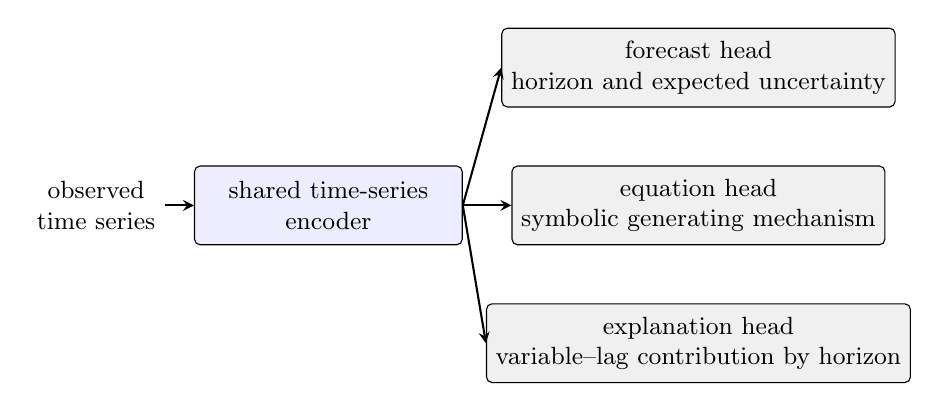
\begin{tikzpicture}[
    block/.style={draw,rounded corners=2pt,fill=blue!7,
        minimum width=3.4cm,minimum height=1.0cm,align=center,font=\small},
    head/.style={draw,rounded corners=2pt,fill=black!6,
        minimum width=4.1cm,minimum height=1.0cm,align=center,font=\small},
    flow/.style={->,>=stealth,draw,line width=0.75pt}
]
    \node[font=\small,align=center] (input) at (-5.2,0)
        {observed\\time series};
    \node[block] (encoder) at (-2.25,0)
        {shared time-series\\encoder};
    \node[head] (forecast) at (2.45,1.75)
        {forecast head\\horizon and expected uncertainty};
    \node[head] (equation) at (2.45,0)
        {equation head\\symbolic generating mechanism};
    \node[head] (explanation) at (2.45,-1.75)
        {explanation head\\variable--lag contribution by horizon};

    \draw[flow] (input)--(encoder);
    \draw[flow] (encoder.east)--(forecast.west);
    \draw[flow] (encoder.east)--(equation.west);
    \draw[flow] (encoder.east)--(explanation.west);
\end{tikzpicture}
\caption{Conceptual multi-task model enabled by the synthetic prior. A shared
encoder feeds a forecasting head, an equation-recovery head, and an
explanation head. The generator supplies the training target for each output,
and the benchmark uses the same information as evaluation ground truth.}
\label{fig:dual-prior-benchmark-motivation}
\end{figure}

\subsection{Research Goal}

The goal of this thesis is to design, implement, and validate a configurable
synthetic benchmark for discrete-time time series. Each dataset will be
produced by a fully known generative mechanism from which several compatible
levels of explanation ground truth can be derived. The benchmark will support
the systematic evaluation of three method families: forecasting models,
symbolic system-identification methods, and XAI techniques. The central
evaluation question is whether these methods recover, use, and explain the
true temporal dependencies of the process.

The generator family will progress from simple to more demanding mechanisms,
including autoregressive dependencies, cross-variable and variable--lag
interactions, nonlinear terms, multiple temporal scales, regime changes,
irrelevant variables, and stochastic components. Depending on the mechanism,
the resulting references will include binary structural dependencies, exact
signed coefficients, realized local coefficient--input contributions, and
attribution-based explanations such as generator-level Shapley values. These
references will be indexed at the target, source-variable, lag, instance, and,
when the generator produces multiple future values, forecast-horizon levels.

Following the expression-first strategy of \citet{dascoli2022deep} and the
learned tree-prior alternative of \citet{meznar2023efficient}, the formula
sampler will construct a valid symbolic tree before generating observations.
The retained tree will act as an executable data-generating function and as the
canonical record from which the benchmark derives its structural,
coefficient-level, local-contribution, and attribution-based references.
Following \citet{bendinelli2023controllable}, an optional retrieval protocol
will expose controlled subsets of this record as hypotheses and measure how
mechanism recovery changes when prior information is complete, partial,
missing, or partially incorrect.

The resulting framework will provide controlled and reproducible comparisons
of predictive accuracy, mechanism recovery, and explanation accuracy. It will
also support tests of whether a black-box forecaster relies on the same
temporal relationships as the true generator or as a symbolic model identified
independently from the generated observations.

\subsection{\texorpdfstring{\hspace{0.45em}Research Question}{Research Question}}

\begin{quote}
\textbf{How can synthetic discrete-time time-series generators with known
generative mechanisms and explanation ground truths be used to benchmark the
ability of forecasting, system-identification, and explainability methods to
recover, use, and explain the underlying temporal dependencies?}
\end{quote}

\paragraph{Three sources of disagreement.}
Let $x$ be a forecasting input, $g$ the known generator, $f$ a forecaster
trained on observations from $g$, and $\widehat g$ a symbolic mechanism
identified independently from those observations. The benchmark separates the
following quantities:

\begin{align}
\varepsilon_{\mathrm{forecast}}(x)
&=d_y\!\left(f(x),g(x)\right),
\label{eq:forecast-error}\\
\varepsilon_{\mathrm{mechanism}}^{*}
&=d_{\mathcal M}\!\left(\mathcal M(\widehat g),\mathcal M(g)\right),
\label{eq:mechanism-error}\\
\varepsilon_{\mathrm{explanation}}(x)
&=d_{\mathcal E}\!\left(A(f,x),E_f(x)\right).
\label{eq:explanation-error}
\end{align}

\noindent\textsuperscript{*}\emph{Applicability of the mechanism error:}
this quantity is evaluated when the method exposes an explicit representation
$\mathcal M(\cdot)$ that can be aligned with the known generator, as occurs in
symbolic system-identification methods and explainable-by-design forecasters.
For an explainable-by-design forecaster, $\mathcal M(\widehat g)$ in
Eq.~\ref{eq:mechanism-error} is replaced by $\mathcal M(f)$. Post-hoc
attribution methods are evaluated through the explanation comparisons in
Eqs.~\ref{eq:explanation-error}--\ref{eq:symbolic-agreement}.

Equation~\ref{eq:forecast-error} measures whether the forecaster returns the
same future values as the generator. Equation~\ref{eq:mechanism-error} measures
whether system identification recovers the generator's structure, lags,
coefficients, nonlinear terms, and regimes at the level represented by
$\mathcal M$. Equation~\ref{eq:explanation-error} measures whether an XAI
method faithfully describes the mechanism actually used by the trained
forecaster; $E_f(x)$ denotes the corresponding model-level reference.

An explainable-by-design forecaster that exposes generator-compatible
source--lag coefficients can also be evaluated through
$d_{\mathcal M}(\mathcal M(f),\mathcal M(g))$, as in the coefficient-recovery
setting studied with DCIts \citep{baric2026dcits}. For a black-box forecaster,
two additional comparisons answer complementary questions:

\begin{align}
\varepsilon_{\mathrm{generator\ agreement}}(x)
&=d_{\mathcal E}\!\left(A(f,x),E_g(x)\right),
\label{eq:generator-agreement}\\
\varepsilon_{\mathrm{symbolic\ agreement}}(x)
&=d_{\mathcal E}\!\left(A(f,x),E_{\widehat g}(x)\right).
\label{eq:symbolic-agreement}
\end{align}

The first comparison tests end-to-end agreement between the black-box
explanation and the true process explanation; it combines any mismatch learned
by $f$ with the behavior of the XAI method. The second tests agreement with an
independently recovered symbolic explanation; its interpretation is paired
with the mechanism-identification error in Eq.~\ref{eq:mechanism-error}. A
small symbolic-agreement error becomes evidence about the true mechanism when
$\widehat g$ also achieves a small mechanism-identification error. Together,
these quantities separate accurate forecasting, recovery of the generating
rule, and faithful explanation of the predictor while allowing their
relationships to be studied explicitly.

\subsection{Benchmark Requirements}
\label{sec:benchmark-requirements}

The benchmark requirements distinguish three kinds of commitment. A
\emph{core requirement} defines behavior that the first complete library must
provide; a \emph{research requirement} identifies a methodological decision
that must be resolved and documented during development; and an
\emph{extension point} keeps the implementation open to later additions
without expanding the experimental scope of this thesis. This distinction is
important because the principal contribution is the generation of executable
time-series mechanisms and their explanation ground truths. General-purpose
grammar design and unrestricted user-defined operators remain extension
points.

\subsubsection{Fixed grammar and reproducible mechanism sampling}

\paragraph{R1: fixed and versioned grammar.}
The project will define one fixed initial vocabulary of constants, lagged
variables, unary operators, binary operators, and mechanism-level constructs.
Users will configure how mechanisms are sampled from this vocabulary, while
the vocabulary itself remains controlled by the project. Every generated
dataset will record a grammar version. Internally, operators will be
registered through a modular interface so that later versions can extend the
grammar without changing the public contract of the first benchmark.

\paragraph{R2: deterministic random generation.}
A global seed, complete generation configuration, library version, and
execution backend will determine the generated mechanisms, coefficients,
initial conditions, innovations, trajectories, windows, and stochastic
explanation estimates. Each artifact will receive a named random stream
derived from stable identifiers such as the mechanism, trajectory, window,
and explanation method. Consequently, changing the number of data-loading
workers or their completion order will preserve the identity and contents of
every indexed example. Repeated execution on the same backend will target
bitwise equality; comparisons across numerical backends will use a declared
floating-point tolerance.

\paragraph{R3: separation between mechanisms and trajectories.}
A mechanism record will contain the expression tree, lag assignments,
coefficients, noise law, and any regime-transition rule. One mechanism may
generate several trajectories. These trajectories share the same symbolic
tree and sampled mechanism parameters while using independently seeded initial
conditions and innovation realizations. This hierarchy supports the study of
whether a method recovers a persistent generating rule rather than properties
of one particular realization:
\[
\boxed{
\text{mechanism}
\longrightarrow
\{\text{trajectory}_{1},\ldots,\text{trajectory}_{K}\}
\longrightarrow
\{\text{forecasting windows}\}.
}
\]
Each window will retain identifiers linking it to its trajectory and canonical
mechanism.

\subsubsection{Controlled and randomly covered difficulty}

\paragraph{R4: two complementary descriptions of difficulty.}
The benchmark will store both \emph{designed difficulty}, determined by the
sampled mechanism, and \emph{measured difficulty}, determined from the
realized forecasting task. Designed difficulty includes tree depth, operator
count, interaction order, number of active variables, lag distance, temporal
scales, recursion depth, regime changes, and the configured noise level.
Measured difficulty includes forecastability statistics, oracle uncertainty,
and the excess error of a fixed panel of reference forecasters over the known
generator.

This separation avoids treating all hard examples as equivalent. A
white-noise process has a simple structural rule but high irreducible
uncertainty, whereas a noiseless nonlinear recurrence can be structurally
complex while remaining deterministic. Difficulty is therefore recorded for
a specified input length, observed-variable set, loss, and horizon. The same
trajectory can be easy at $h=1$ and difficult at a longer horizon.

Related work supplies useful but complementary precedents. SynTSBench controls
temporal pattern families, irregularities, dependencies, and theoretical
optima in order to diagnose forecasting capabilities
\citep{tan2025syntsbench}. The difficulty-conditioned generator of
\citet{cazaux2026synthetic} uses a scalar to alter component balance,
harmonics, regime changes, and noise, and samples named easy, medium, hard, and
uniform distributions. Its downstream ablation also shows that generator
difficulty labels alone need not create proportionally separated forecasting
errors. Data-driven forecastability can additionally be characterized through
spectral predictability and Lyapunov stability \citep{wang2025forecastability}
or through the task-aligned spectral-coherence score of
\citet{feng2025predictability}. These results motivate calibration rather than
assigning difficulty from expression size alone.

\paragraph{R5: random generation with calibrated coverage.}
The default benchmark suite will first sample a target difficulty stratum and
then sample mechanisms from its internal prior. A calibration stage will
measure the realized examples, adjust or relabel them, and freeze versioned
thresholds. The released suite will report the intended stratum and the
measured difficulty descriptors, permitting both a balanced easy--medium--hard
comparison and analysis along the individual axes. Establishing the precise
calibration score and thresholds is a research requirement of the thesis.

\subsubsection{Horizon-aware explanation ground truths}

\paragraph{R6: a separate reference for every forecast step.}
Every explanation ground truth will retain the forecast-horizon axis. For a
source variable $j$, historical offset $d$, and forecast step $h$, the
reference answers whether and how $x_{j,\tau-d}$ affects $g_h(x)$. The canonical
tensor organization is therefore
\[
\boxed{
\text{example}\times
\text{target}\times
\text{horizon}\times
\text{source variable}\times
\text{historical offset},
}
\]
with additional value or method dimensions only when required by a specific
ground-truth family. Aggregation over $h$ will be a reported summary rather
than a replacement for the horizon-resolved reference.

\paragraph{R7: propagation through recursive rollouts.}
When a later forecast uses an earlier generated value, its explanation will be
propagated back to the original observed window. For example, if $g_2(x)$ uses
$g_1(x)$, its input gradient includes both a direct path and the path through
the first forecast:
\begin{equation}
\frac{\partial g_2(x)}{\partial x_{j,\tau-d}}
=
\left.
\frac{\partial g_2(x)}{\partial x_{j,\tau-d}}
\right|_{\mathrm{direct}}
+
\frac{\partial g_2(x)}{\partial g_1(x)}
\frac{\partial g_1(x)}{\partial x_{j,\tau-d}}.
\label{eq:recursive-gradient-requirement}
\end{equation}
Repeated application of Eq.~\eqref{eq:recursive-gradient-requirement}
propagates differentiable effects through the complete rollout. Structural
references will propagate Boolean reachability through the same computation
graph. Generator-level Shapley values will define the value function using the
complete $h$-step rollout, so that coalitions are evaluated directly for the
requested horizon. This is required because Shapley values from consecutive
nonlinear forecast steps cannot in general be combined by simple addition.

\paragraph{R8: selectable ground truths.}
Users will request the ground-truth families needed by an experiment. Binary
structural support can be derived from every retained expression graph. Signed
coefficients apply to mechanisms with identifiable coefficient parameters;
realized local contributions apply when the expression admits a declared
decomposition; and gradients apply to differentiable operators under a stated
policy for nondifferentiable points. Generator-level Shapley values apply to an
executable generator but may require exact enumeration, permutation sampling,
or specialized estimators depending on the number of players. The library will
record the estimator, baseline or conditional sampler, approximation budget,
and uncertainty of every stochastic reference. Gradient feasibility and the
treatment of discontinuities and regime switches are research requirements.

\subsubsection{Model-independent evaluation and explanation metrics}

\paragraph{R9: universal forecasting-model adapter.}
The evaluation layer will interact with a predictor through a small adapter
contract for fitting when required, prediction, and optional explanation or
mechanism retrieval. The contract will represent zero-shot foundation models,
trainable global or local models, statistical models, and
explainable-by-design forecasters. Each adapter will publish capabilities such
as multivariate input, known future covariates, probabilistic output,
automatic differentiation, native explanation, and explicit mechanism
retrieval. Dataset generation and metric implementations will remain
independent of model-specific code.

\paragraph{R10: metrics matched to explanation semantics.}
The benchmark will provide several \emph{explainability} metrics for each
compatible reference family. Binary source--lag masks will use support and
ranking measures such as precision, recall, F1, area under the precision--recall
curve, and top-$k$ recovery. Signed coefficients and signed local references
will additionally use normalized value error and sign agreement. Continuous
attributions will use magnitude error, rank correlation, top-$k$ overlap, sign
agreement, and completeness residuals when completeness belongs to the
attribution definition. Metrics will first be computed per example and
horizon; macro- and micro-aggregated results will be reported separately to
avoid allowing frequent or long mechanisms to dominate every summary.

\paragraph{R11: capability-aware separation of errors.}
Forecast error in Eq.~\eqref{eq:forecast-error} applies whenever an adapter
returns predictions. Explanation comparisons apply when an explainer or model
returns an output aligned with a supported reference. Mechanism-identification
error in Eq.~\eqref{eq:mechanism-error} applies when a method exposes an
explicit, alignable representation. The library will return applicability
metadata alongside every metric rather than filling unsupported comparisons
with inferred values. The exact user-facing adapter and result interfaces, and
the boundary between model-level fidelity and generator agreement, form a
research requirement to be resolved through executable prototypes.

\subsubsection{Lazy, parallel, and batched generation}

\paragraph{R12: PyTorch-compatible on-demand dataset.}
The primary dataset interface will follow the indexed
\texttt{torch.utils.data.Dataset} contract. An index will deterministically
identify a mechanism, trajectory, and forecasting window; requesting that
index will generate or retrieve its values and the selected explanation
ground truths. This map-style interface supports exact replay, stable
train--validation--test partitions, caching, and comparison of multiple models
on identical examples.

The dataset will integrate with \texttt{DataLoader} workers so that future
batches are generated concurrently while the current batch is consumed. The
implementation will support worker processes, custom collation, batch
prefetching, persistent workers, and pinned host memory as described in the
official PyTorch data-loading interface.\footnote{PyTorch data-loading
documentation: \url{https://docs.pytorch.org/docs/stable/data.html}.}
A typical use will have the following form:

\begin{lstlisting}[language=Python,caption={Required lazy and parallel batch-generation interface.}]
dataset = SyntheticExplanationDataset(
    seed=42,
    num_mechanisms=1000,
    trajectories_per_mechanism=10,
    context_length=512,
    prediction_length=96,
    ground_truths=["structural_mask", "gradient"],
)

loader = DataLoader(
    dataset,
    batch_size=64,
    num_workers=8,
    prefetch_factor=2,
    persistent_workers=True,
    pin_memory=True,
    collate_fn=dataset.collate,
)

for batch in loader:
    forecast = model(batch["past_values"])
    report.update(forecast, batch)
\end{lstlisting}

The collated batch will contain the past window, future target, requested
horizon-resolved ground truths, and identifiers for the formula, mechanism,
trajectory, and window. Expensive explanation references will be computed only
when requested and may be stored in a bounded cache. A later streaming
interface may use \texttt{IterableDataset} for effectively unlimited
pretraining data; the indexed dataset remains the reference implementation for
benchmark comparisons.

\paragraph{R13: performance characterization and scalable execution.}
Performance experiments will compare sequential CPU generation,
vectorized CPU execution, CPU multiprocessing, and batched GPU execution.
They will measure examples and batches per second, latency, peak host and
device memory, accelerator utilization, cache hit rate, and the cost of each
ground-truth family. CPU workers will normally produce host tensors and pinned
memory will support asynchronous device transfer. GPU-native generation will
use a controlled batched execution path rather than independent CUDA contexts
inside data-loader workers. The final configuration will preserve the stable
sample identity defined by R2 for every tested worker count and backend.

\subsubsection{Ground-truth correctness and acceptance criteria}

\paragraph{R14: correctness tests for generated references.}
The implementation will include tests of the benchmark's own reference
construction. Executing the stored mechanism must reproduce its deterministic
trajectory before innovations are added; expression leaves must agree with the
structural mask; analytical or automatic gradients must agree with finite
differences away from nondifferentiable points; and multi-horizon toy
recurrences must verify recursive path propagation. Where the attribution
definition requires efficiency, the baseline plus attributed contributions
must reconstruct the relevant output within the estimator's declared
tolerance. Seed, cache, batching, and parallel-worker tests must reproduce the
same indexed examples. These checks establish the internal correctness of the
ground truths before they are used to judge forecasting or explanation
methods.

Table~\ref{tab:benchmark-requirements} summarizes the resulting acceptance
contract.

\begingroup
\small
\renewcommand{\arraystretch}{1.08}
\begin{longtable}{@{}
>{\raggedright\arraybackslash}p{0.08\textwidth}
>{\raggedright\arraybackslash}p{0.42\textwidth}
>{\raggedright\arraybackslash}p{0.42\textwidth}@{}}
\caption{Requirements and acceptance evidence for the proposed benchmark.}
\label{tab:benchmark-requirements}\\
\toprule
ID & Required behavior & Acceptance evidence \\
\midrule
\endfirsthead
\multicolumn{3}{@{}l}{\small\emph{Table~\thetable\ continued}}\\
\toprule
ID & Required behavior & Acceptance evidence \\
\midrule
\endhead
\midrule
\multicolumn{3}{r@{}}{\small\emph{Continued on the next page}}\\
\endfoot
\bottomrule
\endlastfoot
R1 & Fixed, documented, and versioned initial grammar. & Every dataset records its grammar version and every sampled tree validates against that version. \\
R2 & Deterministic named random streams. & Equal configuration, seed, version, and backend produce equal sample hashes; worker count does not change indexed examples. \\
R3 & Multiple trajectories from one retained mechanism. & Trajectories share the tree and mechanism parameters while initial conditions and innovations vary reproducibly. \\
R4 & Separate designed complexity from realized forecastability. & Both descriptor groups are stored per mechanism, trajectory, task, and horizon where applicable. \\
R5 & Random generation covering easy, medium, and hard cases. & A versioned calibration protocol reports intended strata, measured descriptors, thresholds, and final counts. \\
R6 & Horizon-resolved explanation references. & Every supported reference exposes target, horizon, source, and historical-offset axes before aggregation. \\
R7 & Recursive explanation propagation. & Analytical multi-step recurrences verify gradients, structural paths, and complete-rollout attribution behavior. \\
R8 & Optional ground-truth families with explicit applicability. & Output metadata records the reference definition, estimator, configuration, uncertainty, and unsupported cases. \\
R9 & Model-independent evaluation adapter. & Statistical, zero-shot, trainable, black-box, and explainable-by-design examples use the same evaluation entry point. \\
R10 & Explanation-specific metric families. & Binary, signed, ranked, and local-valued references are evaluated only with semantically compatible metrics. \\
R11 & Capability-aware error decomposition. & Reports distinguish computed, unsupported, and inapplicable forecast, mechanism, and explanation comparisons. \\
R12 & Lazy parallel batch generation. & A PyTorch DataLoader generates and prefetches batches without materializing the complete dataset and without duplicated samples. \\
R13 & Measured CPU/GPU performance. & Reproducible profiles report throughput, latency, memory, utilization, caching, and ground-truth cost. \\
R14 & Internal ground-truth correctness tests. & Stored mechanisms, masks, gradients, recursive paths, attributions, seeds, and caches pass automated consistency checks. \\
\end{longtable}
\endgroup

\clearpage
\section{Research Plan}

\subsection{Scope of the November 2026 minimum viable benchmark}

The target for 30 November 2026 is a tested Python library rather than a
single experiment script. Its minimum viable release will (i) sample valid
discrete-time formulas, (ii) execute them to generate reproducible datasets,
(iii) derive several explanation ground truths from the retained formulas,
(iv) accept forecasting models through a small adapter interface, and
(v) produce comparable forecasting and explanation reports. The first release
will prioritize deterministic autoregressive, cross-variable, nonlinear, and
irrelevant-input mechanisms. Regime switching and stochastic mechanisms will
enter the release only after the deterministic path passes its validation
tests, because they introduce additional questions about state labels,
innovation terms, and the object to be explained.

The first stochastic generator will use additive zero-mean Gaussian
innovations with a sampled scale. This initial restriction makes the expected
error distribution explicit and testable. Additional innovation families,
including heavy-tailed, heteroscedastic, and regime-dependent noise, will be
considered after the Gaussian generator and its evaluation interface pass the
validation gates.

The intended dependency order is
\[
\boxed{
\begin{gathered}
\text{formula AST}
\longrightarrow
\text{executable generator}
\longrightarrow
\text{time-series dataset}
\\[1mm]
\Downarrow
\\[1mm]
\text{explanation ground truths}
\longrightarrow
\text{model adapters}
\longrightarrow
\text{evaluation}
\end{gathered}
}.
\]
Consequently, model experiments do not begin before both the observations and
their references can be generated and checked. A lightweight software
interface is specified early so that the generator does not become tied to one
forecasting package, but the interface is exercised on real models only after
the ground-truth layer is complete.

\subsection{Formula sampler}

Following the expression-first strategy of \citet{dascoli2022deep}, the
sampler will first create an abstract syntax tree (AST) and only then execute
it. Let $\mathcal E$ denote a valid symbolic expression, either the complete
right-hand side of a recurrence or one of its subexpressions. A minimal
recursive grammar is
\[
\begin{aligned}
\mathcal E ::= {}& c
&& \text{sampled constant,}\\
&\mid \operatorname{LAG}(j,\ell)
&& \text{series $j$ observed $\ell$ steps earlier,}\\
&\mid \operatorname{ADD}(\mathcal E_1,\mathcal E_2)
&& \text{sum of two valid expressions,}\\
&\mid \operatorname{MUL}(\mathcal E_1,\mathcal E_2)
&& \text{product of two valid expressions,}\\
&\mid \operatorname{UNARY}_{\varphi}(\mathcal E_1)
&& \text{unary function applied to one expression,}
\end{aligned}
\qquad \ell\geq 1.
\]
The symbol $\mathcal E$ is therefore a grammar non-terminal: it is a
placeholder for any expression that can be constructed by repeatedly applying
these rules. The symbols $\mathcal E_1$ and $\mathcal E_2$ are child
expressions constructed by the same grammar, $c$ is a sampled constant, $j$
identifies a source series, and $\varphi$ is selected from a controlled set of
safe unary functions.

For example, the symbolic tree
\[
\begin{aligned}
\mathcal E={}&\operatorname{ADD}\!\bigl(
    \operatorname{MUL}(0.7,\operatorname{LAG}(1,1)),\\
&\hspace{38mm}\operatorname{SIN}(\operatorname{LAG}(1,3))
\bigr)
\end{aligned}
\]
is executed as the recurrence
\[
x_{1,t}=0.7x_{1,t-1}+\sin(x_{1,t-3}).
\]
Extensions will add explicit interaction, regime, multiscale, and innovation
nodes. The AST is retained alongside every series as the canonical description
of the mechanism; a rendered equation is a human-readable view of that same
object.

The sampler must control tree depth, operator counts, admissible domains,
maximum lag, coefficient ranges, and duplicated or inactive branches. Candidate
formulas are rejected when short pilot simulations diverge, collapse to an
almost constant series, produce non-finite values, or fail to use the sampled
dependencies. Each accepted formula is serialized with its seed and complete
parameter record so that it can be reconstructed exactly.

\subsection{Series generation and dataset contract}

For target series $k$, the AST is compiled into an executable recurrence
\[
x_{k,t}=g_{k,1}\!\left(x_{:,t-1},\ldots,x_{:,t-L};\theta\right)
       +\varepsilon_{k,t}.
\]
Initial conditions are sampled first, a burn-in interval is discarded, and the
remaining observations are divided chronologically into training, validation,
and test windows. The generator records the formula, coefficients, initial
conditions, innovations, regime sequence when applicable, seeds, window
boundaries, and temporal convention. This metadata distinguishes the process
that generated the observations from the input window later presented to a
model.

Multi-step reference outputs are produced by recursively executing the known
generator. Thus $g_{k,h}$ denotes the output at horizon $h$ after unrolling the
one-step recurrence $h$ times. The benchmark will expose the same sample through
a canonical batch containing observed history, optional known future
covariates, target values, horizon, masks, and metadata. An adapter may transform
that batch into a package-specific dataframe or tensor, but it cannot silently
change which information the model receives.

\subsection{Explanation ground truths}

Only after an accepted formula and its observations exist does the library
derive explanation references. One generated example can expose four
compatible views:

\begin{enumerate}
    \item a binary source--lag support extracted from the AST and, for
    $h>1$, from the recursively unrolled dependency graph;
    \item signed coefficients for mechanisms whose effect is represented by a
    coefficient, together with realized coefficient--input terms;
    \item a local gradient reference
    \[
    G^{\mathrm{grad}}_{n,h,j,d}
      =\frac{\partial g_{k,h}(x_n)}
             {\partial x_{j,\tau-d}},
    \]
    computed by automatic differentiation when the sampled operators are
    differentiable and checked against finite differences; and
    \item generator-level Shapley values obtained by evaluating the executable
    generator under feature coalitions and a declared conditional resampling
    rule; when the benchmark declares a hierarchy of player groups, the same
    game also yields Owen values that respect that grouping.
\end{enumerate}

The raw gradient measures local sensitivity. A baseline-relative
gradient--input quantity,
$(x_{j,\tau-d}-b_{j,d})G^{\mathrm{grad}}_{n,h,j,d}$, may also be stored, but it
will be named separately because it is a contribution heuristic rather than a
Shapley value. Comparisons remain within the same explanation family: a model
gradient is compared with the generator gradient, while a model SHAP
explanation is compared with the generator SHAP reference. Exact Shapley
enumeration will validate small cases; permutation sampling and caching will be
used when the number of players makes enumeration impractical.

\subsection{Model-independent evaluation layer}

The public boundary of the benchmark is a \texttt{ForecastAdapter}. Every
adapter declares its input capabilities and implements fitting, prediction,
and, when available, access to an intrinsic mechanism or differentiable model.
The evaluator will therefore distinguish three cases:

\begin{itemize}
    \item every adapter can be evaluated for forecast accuracy;
    \item any callable predictor can receive model-agnostic perturbation or
    finite-difference explanations;
    \item mechanism-recovery metrics are computed only when a method exposes a
    generator-compatible structure, equation, coefficient tensor, or other
    explicit mechanism. Unsupported cells are reported as not applicable, not
    as zero performance.
\end{itemize}

The initial integration set comprises Chronos-2
\citep{ansari2025chronos2}, Toto 2.0 from Datadog
\citep{khwaja2026toto2}, AutoARIMA \citep{hyndman2008auto}, and, as an
optional explainable-by-design baseline, DCIts \citep{baric2026dcits}. The
planning name ``Kronos-2'' is normalized here to \emph{Chronos-2}; Kronos is a
different foundation model specialized for financial-market sequences.
Chronos-2 and Toto 2.0 are evaluated as pretrained forecasters through their
adapters. AutoARIMA is evaluated first with target-only history; a separate
ARIMAX configuration can later receive declared exogenous variables. DCIts
provides a learned transition tensor rather than a symbolic equation, so its
native coefficients can be compared with compatible generator references.

Forecast metrics will include MAE, RMSE, and MASE. Structural recovery will use
precision, recall, and F1 over source--lag support. Coefficient recovery will
use signed error and sign agreement when such coefficients exist. Local
explanation comparisons will include normalized attribution error, rank
correlation, top-$q$ overlap, and sign agreement. All results will retain the
instance, target, horizon, source variable, lag, operator family, formula
complexity, and random seed required for stratified analysis.

\subsection{Validation gates}

The release is accepted only if (i) AST parsing and serialization round-trip
without changing a formula, (ii) seeded generation is reproducible, (iii)
hand-derived support, coefficient, contribution, gradient, and small Shapley
examples match the implementation, (iv) one-step and recursively unrolled
horizon references are separated, (v) all model adapters receive the declared
input only, and (vi) the complete pipeline runs from configuration file to
tables without notebook-only state. These gates protect the benchmark from
producing precise-looking metrics for an incorrectly represented mechanism.

\subsection{Weekly plan}

Table~\ref{tab:weekly-plan} places formula and series generation before the
explanation layer, and places the model study after both. Each week ends in a
testable artifact rather than an open-ended research activity.

Figure~\ref{fig:research-plan-gantt} presents the same plan as a dependency-aware
Gantt chart. Solid arrows mark hard gates. The dashed region identifies work
that can proceed in parallel once the executable generator has passed its first
validation gate; the adapter contract begins earlier from the frozen data
contract, but its implementation converges with the dataset and explanation
branches before model integration.

\begin{landscape}
\begin{figure}[H]
    \centering
    \resizebox{0.98\linewidth}{!}{%
        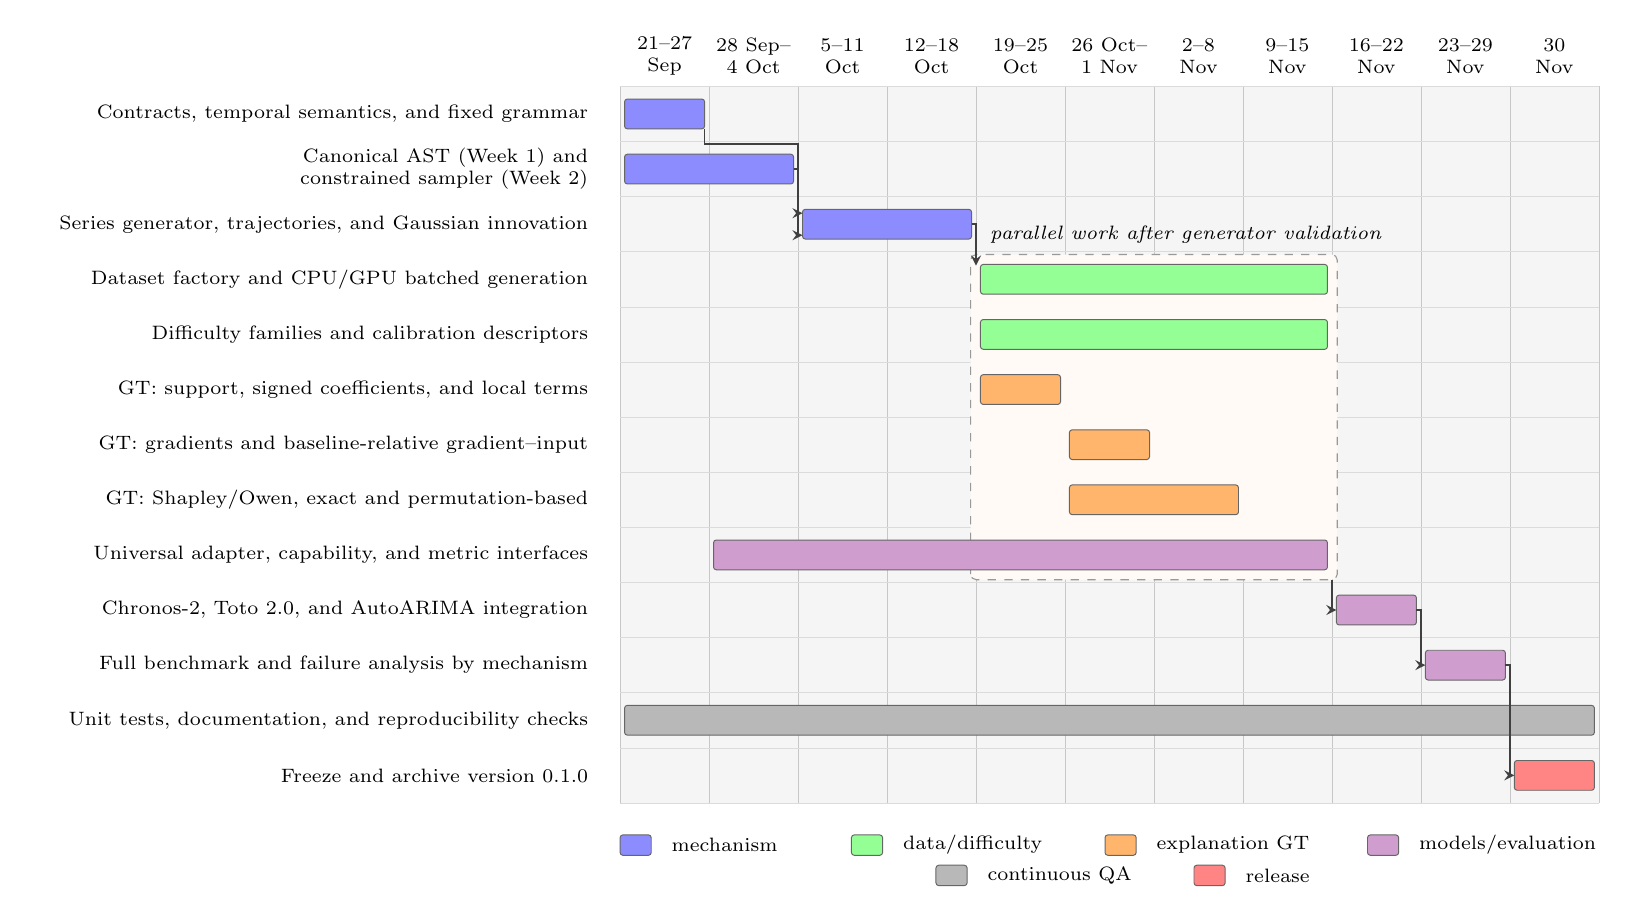
\begin{tikzpicture}[
    x=1.13cm,
    y=0.70cm,
    tasklabel/.style={font=\scriptsize,anchor=east,align=right,text width=7.0cm},
    bar/.style={draw=black!60,line width=0.35pt,rounded corners=1pt},
    dependency/.style={->,>=stealth,semithick,draw=black!75},
    legend/.style={font=\scriptsize,anchor=west}
]

% Timeline grid.
\fill[black!4] (0,-0.5) rectangle (11,12.5);
\foreach \x in {0,...,11} {
    \draw[black!22,line width=0.25pt] (\x,-0.5) -- (\x,12.5);
}
\foreach \y in {-0.5,0.5,...,12.5} {
    \draw[black!14,line width=0.2pt] (0,\y) -- (11,\y);
}

% Week headings.
\node[font=\scriptsize,align=center] at (0.5,13.05) {21--27\\Sep};
\node[font=\scriptsize,align=center] at (1.5,13.05) {28 Sep--\\4 Oct};
\node[font=\scriptsize,align=center] at (2.5,13.05) {5--11\\Oct};
\node[font=\scriptsize,align=center] at (3.5,13.05) {12--18\\Oct};
\node[font=\scriptsize,align=center] at (4.5,13.05) {19--25\\Oct};
\node[font=\scriptsize,align=center] at (5.5,13.05) {26 Oct--\\1 Nov};
\node[font=\scriptsize,align=center] at (6.5,13.05) {2--8\\Nov};
\node[font=\scriptsize,align=center] at (7.5,13.05) {9--15\\Nov};
\node[font=\scriptsize,align=center] at (8.5,13.05) {16--22\\Nov};
\node[font=\scriptsize,align=center] at (9.5,13.05) {23--29\\Nov};
\node[font=\scriptsize,align=center] at (10.5,13.05) {30\\Nov};

% Task labels.
\node[tasklabel] at (-0.25,12) {Contracts, temporal semantics, and fixed grammar};
\node[tasklabel] at (-0.25,11) {Canonical AST (Week 1) and constrained sampler (Week 2)};
\node[tasklabel] at (-0.25,10) {Series generator, trajectories, and Gaussian innovation};
\node[tasklabel] at (-0.25,9) {Dataset factory and CPU/GPU batched generation};
\node[tasklabel] at (-0.25,8) {Difficulty families and calibration descriptors};
\node[tasklabel] at (-0.25,7) {GT: support, signed coefficients, and local terms};
\node[tasklabel] at (-0.25,6) {GT: gradients and baseline-relative gradient--input};
\node[tasklabel] at (-0.25,5) {GT: Shapley/Owen, exact and permutation-based};
\node[tasklabel] at (-0.25,4) {Universal adapter, capability, and metric interfaces};
\node[tasklabel] at (-0.25,3) {Chronos-2, Toto 2.0, and AutoARIMA integration};
\node[tasklabel] at (-0.25,2) {Full benchmark and failure analysis by mechanism};
\node[tasklabel] at (-0.25,1) {Unit tests, documentation, and reproducibility checks};
\node[tasklabel] at (-0.25,0) {Freeze and archive version 0.1.0};

% Parallel work window after the first validated generator.
\filldraw[fill=orange!4,draw=black!40,dashed,rounded corners=2pt]
    (3.94,3.55) rectangle (8.06,9.45);
\node[font=\scriptsize\itshape,anchor=south west] at (4.05,9.48)
    {parallel work after generator validation};

% Core mechanism construction.
\filldraw[bar,fill=blue!45] (0.05,11.73) rectangle (0.95,12.27);
\filldraw[bar,fill=blue!45] (0.05,10.73) rectangle (1.95,11.27);
\filldraw[bar,fill=blue!45] (2.05,9.73) rectangle (3.95,10.27);

% Scalable generation and controlled difficulty.
\filldraw[bar,fill=green!42] (4.05,8.73) rectangle (7.95,9.27);
\filldraw[bar,fill=green!42] (4.05,7.73) rectangle (7.95,8.27);

% Explanation-ground-truth methods.
\filldraw[bar,fill=orange!58] (4.05,6.73) rectangle (4.95,7.27);
\filldraw[bar,fill=orange!58] (5.05,5.73) rectangle (5.95,6.27);
\filldraw[bar,fill=orange!58] (5.05,4.73) rectangle (6.95,5.27);

% Evaluation interface and model study.
\filldraw[bar,fill=violet!38] (1.05,3.73) rectangle (7.95,4.27);
\filldraw[bar,fill=violet!38] (8.05,2.73) rectangle (8.95,3.27);
\filldraw[bar,fill=violet!38] (9.05,1.73) rectangle (9.95,2.27);

% Continuous quality work and final milestone.
\filldraw[bar,fill=black!28] (0.05,0.73) rectangle (10.95,1.27);
\filldraw[bar,fill=red!48] (10.05,-0.27) rectangle (10.95,0.27);

% Hard dependency gates.
\draw[dependency] (0.95,11.73) -- (0.95,11.45) -- (2.00,11.45)
    -- (2.00,10.20) -- (2.05,10.20);
\draw[dependency] (1.95,11) -- (2.00,11) -- (2.00,9.80) -- (2.05,9.80);
\draw[dependency] (3.95,10) -- (4.00,10) -- (4.00,9.25);
\draw[dependency] (8.00,3.55) -- (8.00,3) -- (8.05,3);
\draw[dependency] (8.95,3) -- (9.00,3) |- (9.05,2);
\draw[dependency] (9.95,2) -- (10.00,2) -- (10.00,0) -- (10.05,0);

% Legend, split over two rows to remain readable after page scaling.
\filldraw[bar,fill=blue!45] (0,-1.45) rectangle (0.35,-1.08);
\node[legend] at (0.47,-1.265) {mechanism};
\filldraw[bar,fill=green!42] (2.60,-1.45) rectangle (2.95,-1.08);
\node[legend] at (3.07,-1.265) {data/difficulty};
\filldraw[bar,fill=orange!58] (5.45,-1.45) rectangle (5.80,-1.08);
\node[legend] at (5.92,-1.265) {explanation GT};
\filldraw[bar,fill=violet!38] (8.40,-1.45) rectangle (8.75,-1.08);
\node[legend] at (8.87,-1.265) {models/evaluation};

\filldraw[bar,fill=black!28] (3.55,-2.00) rectangle (3.90,-1.63);
\node[legend] at (4.02,-1.815) {continuous QA};
\filldraw[bar,fill=red!48] (6.45,-2.00) rectangle (6.80,-1.63);
\node[legend] at (6.92,-1.815) {release};

\end{tikzpicture}
%
    }
    \caption{Dependency-aware Gantt plan for the benchmark release on
    30 November 2026. The explanation-ground-truth branch explicitly covers
    binary source--lag support, signed coefficients and realized local terms,
    automatic-differentiation gradients and gradient--input values, and
    generator-level Shapley values or Owen values for grouped players. Exact
    coalition enumeration is used for small games and permutation estimation
    for larger games.}
    \label{fig:research-plan-gantt}
\end{figure}
\end{landscape}

\begin{landscape}
\begin{figure}[H]
    \centering
    \resizebox{0.77\linewidth}{!}{%
        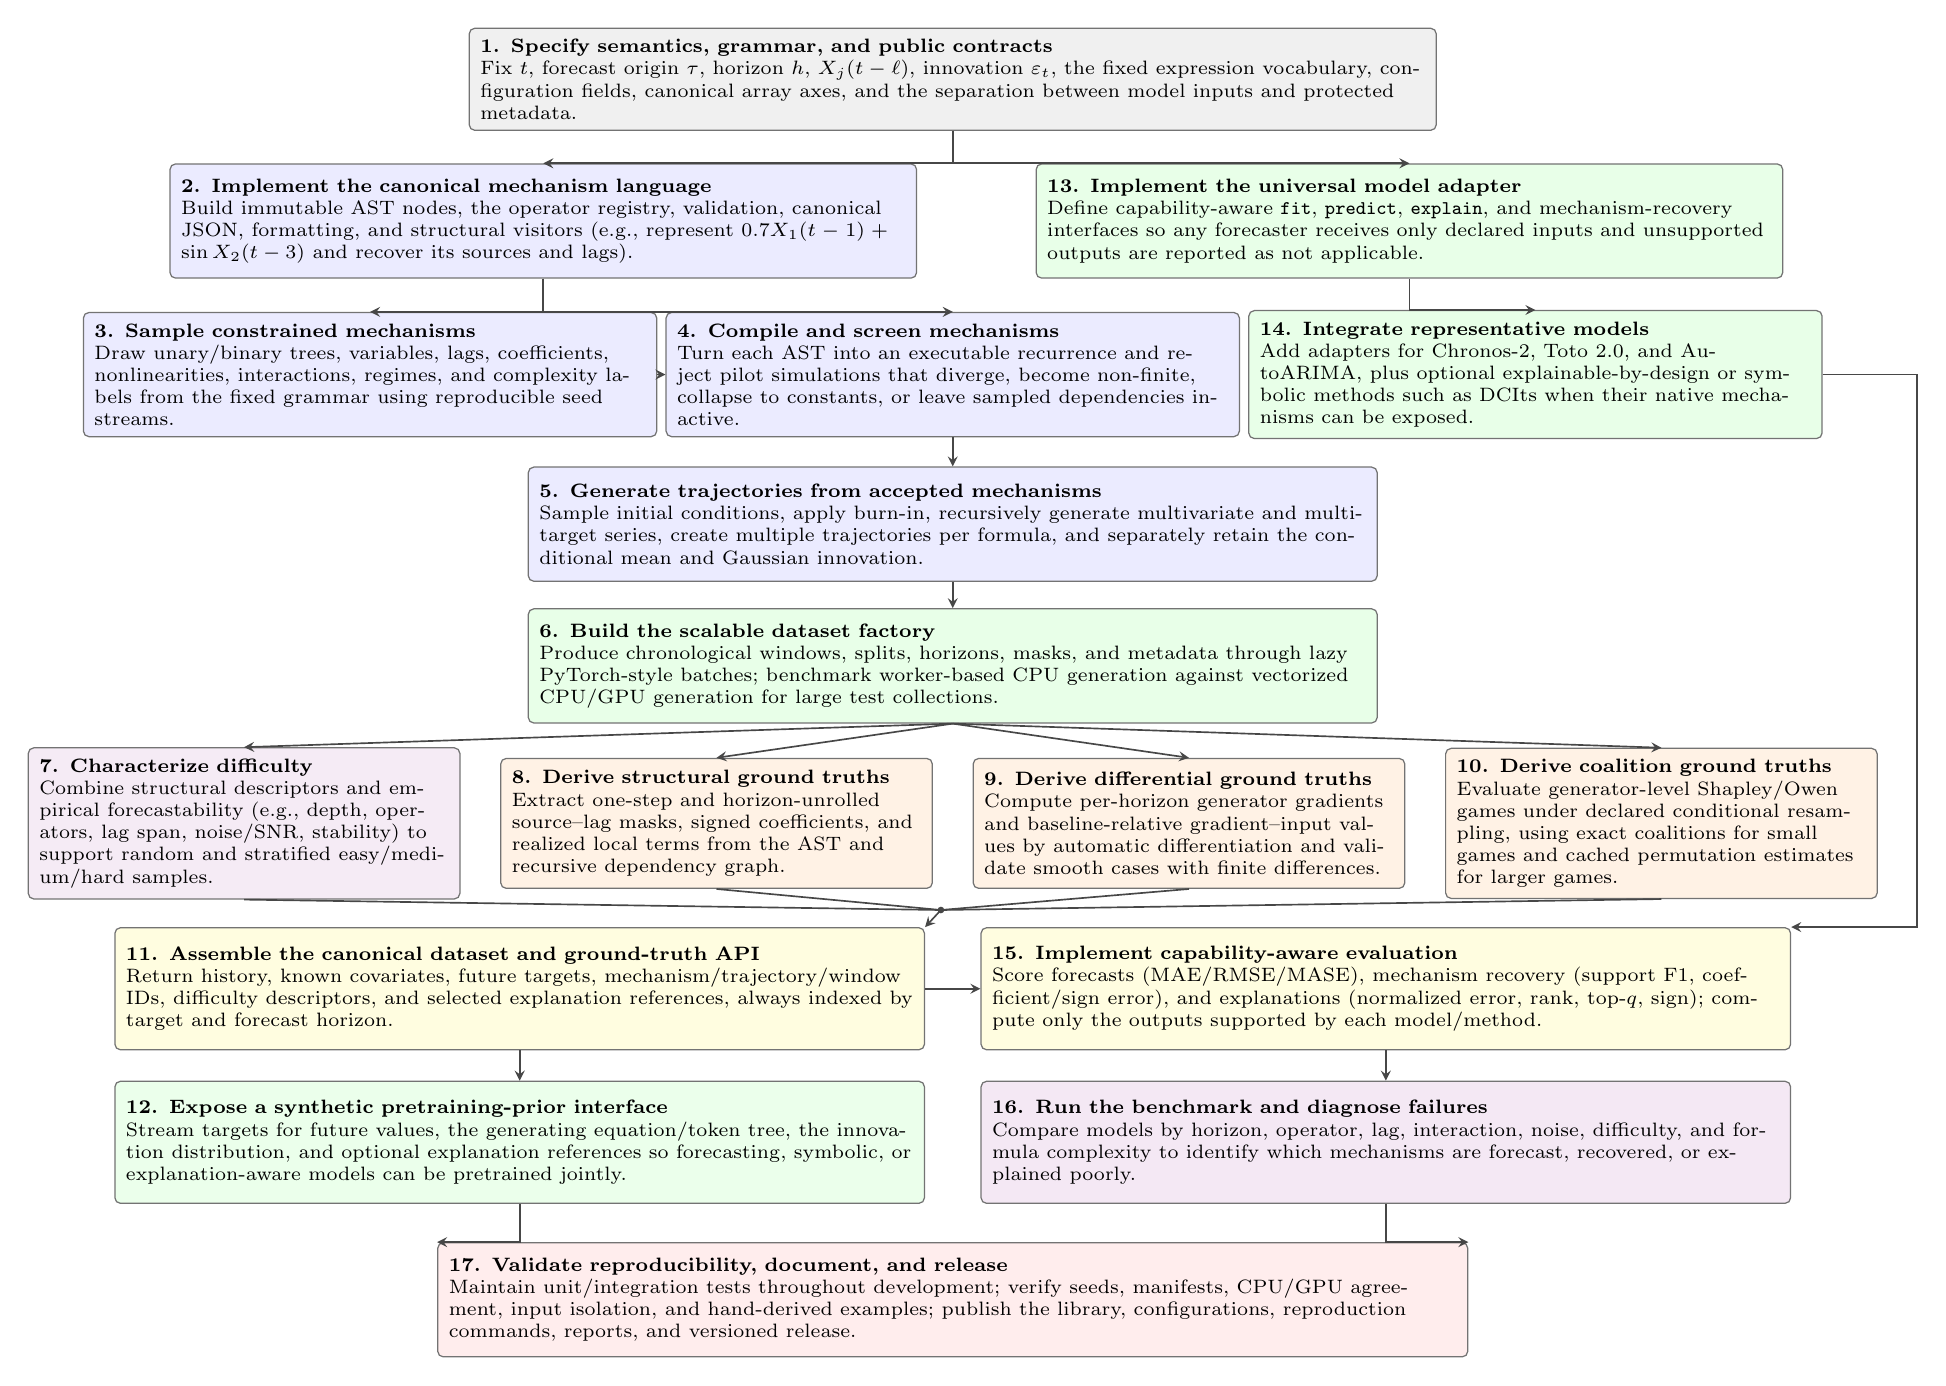
\begin{tikzpicture}[
    x=1cm,
    y=1cm,
    task/.style={
        draw=black!55,
        line width=0.45pt,
        rounded corners=2pt,
        align=left,
        inner sep=4pt,
        font=\scriptsize
    },
    dependency/.style={->,>=stealth,semithick,draw=black!72},
    joinline/.style={semithick,draw=black!72}
]

% Shared scientific and software foundation.
\node[task,fill=black!6,text width=12.0cm,minimum height=1.25cm] (specification) at (0,7.4) {%
    \textbf{1. Specify semantics, grammar, and public contracts}\par
    Fix $t$, forecast origin $\tau$, horizon $h$, $X_j(t-\ell)$, innovation
    $\varepsilon_t$, the fixed expression vocabulary, configuration fields,
    canonical array axes, and the separation between model inputs and protected metadata.
};

\node[task,fill=blue!8,text width=9.2cm,minimum height=1.45cm] (language) at (-5.2,5.6) {%
    \textbf{2. Implement the canonical mechanism language}\par
    Build immutable AST nodes, the operator registry, validation, canonical JSON,
    formatting, and structural visitors (e.g., represent
    $0.7X_1(t-1)+\sin X_2(t-3)$ and recover its sources and lags).
};

% The adapter boundary can start from the public contracts while generators are built.
\node[task,fill=green!9,text width=9.2cm,minimum height=1.45cm] (adapter) at (5.8,5.6) {%
    \textbf{13. Implement the universal model adapter}\par
    Define capability-aware \texttt{fit}, \texttt{predict}, \texttt{explain}, and
    mechanism-recovery interfaces so any forecaster receives only declared inputs and
    unsupported outputs are reported as not applicable.
};

\node[task,fill=blue!8,text width=7.0cm,minimum height=1.55cm] (sampler) at (-7.4,3.65) {%
    \textbf{3. Sample constrained mechanisms}\par
    Draw unary/binary trees, variables, lags, coefficients, nonlinearities,
    interactions, regimes, and complexity labels from the fixed grammar using
    reproducible seed streams.
};

\node[task,fill=blue!8,text width=7.0cm,minimum height=1.55cm] (compiler) at (0,3.65) {%
    \textbf{4. Compile and screen mechanisms}\par
    Turn each AST into an executable recurrence and reject pilot simulations that
    diverge, become non-finite, collapse to constants, or leave sampled dependencies
    inactive.
};

\node[task,fill=green!9,text width=7.0cm,minimum height=1.55cm] (models) at (7.4,3.65) {%
    \textbf{14. Integrate representative models}\par
    Add adapters for Chronos-2, Toto~2.0, and AutoARIMA, plus optional
    explainable-by-design or symbolic methods such as DCIts when their native
    mechanisms can be exposed.
};

\node[task,fill=blue!8,text width=10.5cm,minimum height=1.45cm] (trajectories) at (0,1.75) {%
    \textbf{5. Generate trajectories from accepted mechanisms}\par
    Sample initial conditions, apply burn-in, recursively generate multivariate and
    multi-target series, create multiple trajectories per formula, and separately
    retain the conditional mean and Gaussian innovation.
};

\node[task,fill=green!9,text width=10.5cm,minimum height=1.45cm] (dataset) at (0,-0.05) {%
    \textbf{6. Build the scalable dataset factory}\par
    Produce chronological windows, splits, horizons, masks, and metadata through lazy
    PyTorch-style batches; benchmark worker-based CPU generation against vectorized
    CPU/GPU generation for large test collections.
};

% Parallel products derived from the retained mechanism and generated observations.
\node[task,fill=violet!8,text width=5.2cm,minimum height=1.65cm] (difficulty) at (-9.0,-2.05) {%
    \textbf{7. Characterize difficulty}\par
    Combine structural descriptors and empirical forecastability (e.g., depth,
    operators, lag span, noise/SNR, stability) to support random and stratified
    easy/medium/hard samples.
};

\node[task,fill=orange!10,text width=5.2cm,minimum height=1.65cm] (structural) at (-3.0,-2.05) {%
    \textbf{8. Derive structural ground truths}\par
    Extract one-step and horizon-unrolled source--lag masks, signed coefficients, and
    realized local terms from the AST and recursive dependency graph.
};

\node[task,fill=orange!10,text width=5.2cm,minimum height=1.65cm] (gradient) at (3.0,-2.05) {%
    \textbf{9. Derive differential ground truths}\par
    Compute per-horizon generator gradients and baseline-relative gradient--input
    values by automatic differentiation and validate smooth cases with finite
    differences.
};

\node[task,fill=orange!10,text width=5.2cm,minimum height=1.65cm] (coalition) at (9.0,-2.05) {%
    \textbf{10. Derive coalition ground truths}\par
    Evaluate generator-level Shapley/Owen games under declared conditional resampling,
    using exact coalitions for small games and cached permutation estimates for larger
    games.
};

\node[task,fill=yellow!12,text width=10.0cm,minimum height=1.55cm] (canonicalapi) at (-5.5,-4.15) {%
    \textbf{11. Assemble the canonical dataset and ground-truth API}\par
    Return history, known covariates, future targets, mechanism/trajectory/window IDs,
    difficulty descriptors, and selected explanation references, always indexed by
    target and forecast horizon.
};

\node[task,fill=yellow!12,text width=10.0cm,minimum height=1.55cm] (evaluation) at (5.5,-4.15) {%
    \textbf{15. Implement capability-aware evaluation}\par
    Score forecasts (MAE/RMSE/MASE), mechanism recovery (support F1, coefficient/sign
    error), and explanations (normalized error, rank, top-$q$, sign); compute only the
    outputs supported by each model/method.
};

% Two intended uses of the generated data and ground truths.
\node[task,fill=green!8,text width=10.0cm,minimum height=1.55cm] (prior) at (-5.5,-6.10) {%
    \textbf{12. Expose a synthetic pretraining-prior interface}\par
    Stream targets for future values, the generating equation/token tree, the
    innovation distribution, and optional explanation references so forecasting,
    symbolic, or explanation-aware models can be pretrained jointly.
};

\node[task,fill=violet!9,text width=10.0cm,minimum height=1.55cm] (benchmark) at (5.5,-6.10) {%
    \textbf{16. Run the benchmark and diagnose failures}\par
    Compare models by horizon, operator, lag, interaction, noise, difficulty, and
    formula complexity to identify which mechanisms are forecast, recovered, or
    explained poorly.
};

\node[task,fill=red!7,text width=12.8cm,minimum height=1.45cm] (release) at (0,-8.10) {%
    \textbf{17. Validate reproducibility, document, and release}\par
    Maintain unit/integration tests throughout development; verify seeds, manifests,
    CPU/GPU agreement, input isolation, and hand-derived examples; publish the library,
    configurations, reproduction commands, reports, and versioned release.
};

% Hard technical dependencies.
\draw[dependency] (specification.south) -- ++(0,-0.22) |- (language.north);
\draw[dependency] (specification.south) -- ++(0,-0.22) |- (adapter.north);

\draw[dependency] (language.south) -- ++(0,-0.22) |- (sampler.north);
\draw[dependency] (language.south) -- ++(0,-0.22) |- (compiler.north);
\draw[dependency] (sampler.east) -- (compiler.west);
\draw[dependency] (compiler.south) -- (trajectories.north);
\draw[dependency] (trajectories.south) -- (dataset.north);

\draw[dependency] (adapter.south) -- ++(0,-0.22) |- (models.north);

\draw[dependency] (dataset.south) -- (difficulty.north);
\draw[dependency] (dataset.south) -- (structural.north);
\draw[dependency] (dataset.south) -- (gradient.north);
\draw[dependency] (dataset.south) -- (coalition.north);

\coordinate (productjoin) at (-0.15,-3.15);
\draw[joinline] (difficulty.south) -- (productjoin);
\draw[joinline] (structural.south) -- (productjoin);
\draw[joinline] (gradient.south) -- (productjoin);
\draw[joinline] (coalition.south) -- (productjoin);
\fill[black!72] (productjoin) circle (1.2pt);
\draw[dependency] (productjoin) -- (canonicalapi.north east);

\draw[dependency] (canonicalapi.south) -- (prior.north);
\draw[dependency] (canonicalapi.east) -- (evaluation.west);
\draw[dependency] (models.east) -- ++(1.2,0) |- (evaluation.north east);
\draw[dependency] (evaluation.south) -- (benchmark.north);

\draw[dependency] (prior.south) -- ++(0,-0.22) |- (release.north west);
\draw[dependency] (benchmark.south) -- ++(0,-0.22) |- (release.north east);

\end{tikzpicture}
%
    }
    \caption{Overall technical dependency graph for the project.  The retained
    symbolic mechanism drives trajectory generation, difficulty characterization,
    and structural, differential, and coalition-based explanation references.  The
    resulting API supports two consumers: synthetic pretraining priors and a
    model-agnostic benchmark with capability-aware forecast, mechanism-recovery,
    and explanation evaluation.}
    \label{fig:project-dependency-graph}
\end{figure}
\end{landscape}

\begingroup
\small
\setlength{\LTpre}{0.4\baselineskip}
\setlength{\LTpost}{0.7\baselineskip}
\renewcommand{\arraystretch}{1.08}
\begin{longtable}{@{}
>{\raggedright\arraybackslash}p{0.14\textwidth}
>{\raggedright\arraybackslash}p{0.25\textwidth}
>{\raggedright\arraybackslash}p{0.28\textwidth}
>{\raggedright\arraybackslash}p{0.25\textwidth}@{}}
\caption{Dependency-aware schedule for a usable benchmark by 30 November 2026.}
\label{tab:weekly-plan}\\
\toprule
Dates & Main work & Deliverable & Acceptance criterion \\
\midrule
\endfirsthead
\multicolumn{4}{@{}l}{\small\emph{Table~\thetable\ continued}}\\
\toprule
Dates & Main work & Deliverable & Acceptance criterion \\
\midrule
\endhead
\midrule
\multicolumn{4}{r@{}}{\small\emph{Continued on the next page}}\\
\endfoot
\bottomrule
\endlastfoot

21--27 Sep. &
Freeze temporal semantics, AST schema, operator registry, and configuration
contract. &
Grammar specification, Python types, and hand-written reference formulas. &
At least 30 representative formulas parse, serialize, and preserve their
source--lag identities. \\

28 Sep.--4 Oct. &
Implement constrained random AST sampling and formula rejection filters. &
Seeded formula sampler with complexity and operator labels. &
A batch of 10,000 candidates is reproducible; every accepted formula is
causal, finite in pilot execution, and reconstructible from metadata. \\

5--11 Oct. &
Compile ASTs and implement initial conditions, burn-in, recursive simulation,
and multivariate output. &
Executable deterministic generator and unit tests. &
Repeated seeds reproduce identical series; simple AR, cross-lag, and nonlinear
examples match hand calculations. \\

12--18 Oct. &
Create dataset splits and controlled families for interactions, irrelevant
variables, lag ranges, and temporal scales. &
Versioned dataset factory and data cards. &
Every sample links back to one formula; leakage checks pass and all information
available to a model is recorded explicitly. \\

19--25 Oct. &
Extract structural support, signed coefficients where defined, realized local
terms, and horizon-unrolled dependencies. &
First ground-truth API and visual sanity reports. &
Hand-derived one-step and multi-step examples match the stored masks and
values exactly. \\

26 Oct.--1 Nov. &
Implement generator gradients and baseline-relative gradient--input outputs. &
Gradient reference module indexed by instance, horizon, variable, and lag. &
Autodiff agrees with central finite differences on smooth formulas; undefined
or non-smooth cases are flagged rather than silently scored. \\

2--8 Nov. &
Implement coalition construction, dependency-aware resampling, exact small
Shapley cases, and permutation estimates. &
Generator SHAP reference module with uncertainty and sampling metadata. &
Exact and sampled results agree within a declared tolerance on small formulas,
and efficiency is checked whenever the chosen game satisfies it. \\

9--15 Nov. &
Implement adapter protocols, forecast/mechanism/explanation metrics, capability
checks, and result schema. &
End-to-end library pipeline using naive and oracle test adapters. &
One configuration produces datasets, references, predictions, explanations,
and stratified tables without notebook state. \\

16--22 Nov. &
Integrate Chronos-2, Toto 2.0, and target-only AutoARIMA; add DCIts if the core
path remains on schedule. &
Model adapters and a common pilot experiment. &
Every model sees the documented context and horizon; unsupported mechanism
metrics are marked not applicable. \\

23--29 Nov. &
Run the comparison matrix; analyze error by operator, lag range, horizon,
interaction, and irrelevant-variable count; finish tests and documentation. &
Release candidate, examples, metric tables, and reproducibility manifest. &
A clean environment can reproduce the principal tables from one command and
all mandatory tests pass. \\

30 Nov. &
Freeze and archive version 0.1.0. &
Installable package, tagged configuration set, generated artifacts, and usage
example. &
The release checklist and a full smoke test pass from installation through
report export. \\
\end{longtable}
\endgroup

\subsection{Final goal: using the benchmark as a library}

The final user should configure a generator once and evaluate multiple models
without changing the data-generation or scoring code. Listing~\ref{lst:final-api}
illustrates the intended public API. The adapter classes belong to the proposed
library; internally, they translate the canonical benchmark batch to the
official input expected by each external package.

\begin{lstlisting}[language=Python,caption={Intended end-state API for generating one benchmark and evaluating the prioritized models.},label={lst:final-api}]
from tsxai_benchmark import Benchmark, GeneratorSpec
from tsxai_benchmark.ground_truth import (
    StructuralSupport,
    SignedCoefficients,
    LocalContributions,
    GeneratorGradient,
    GradientInput,
    GeneratorShapley,
)
from tsxai_benchmark.models import (
    Chronos2Adapter,
    Toto2Adapter,
    AutoARIMAAdapter,
    DCItsAdapter,
)
from tsxai_benchmark.xai import InputGradient, PermutationSHAP

# 1. Sample formulas, execute them, and retain every mechanism.
benchmark = Benchmark.generate(
    GeneratorSpec(
        n_formulas=500,
        series_length=1024,
        context_length=256,
        horizon=24,
        max_lag=48,
        operators=["add", "multiply", "sin", "square"],
        include_irrelevant_variables=True,
        seed=42,
    ),
    ground_truths=[
        StructuralSupport(unroll_horizon=True),
        SignedCoefficients(when_defined=True),
        LocalContributions(),
        GeneratorGradient(),
        GradientInput(baseline="training_mean"),
        GeneratorShapley(
            masker="generator_conditional",
            permutations=512,
        ),
    ],
)

# 2. Model-specific details are isolated inside adapters.
models = [
    Chronos2Adapter(model_id="amazon/chronos-2"),
    Toto2Adapter(model_id="Datadog/Toto-2.0-22m"),
    AutoARIMAAdapter(
        season_length=24,
        input_mode="target_only",
    ),
    # Optional explainable-by-design baseline.
    DCItsAdapter(context_length=48),
]

# 3. Like is compared with like: gradients with gradients,
#    and SHAP values with generator-level Shapley values.
report = benchmark.evaluate(
    models=models,
    explainers={
        "gradient": InputGradient(fallback="finite_difference"),
        "shap": PermutationSHAP(
            masker=benchmark.conditional_sampler,
            permutations=512,
        ),
    },
    forecast_metrics=["mae", "rmse", "mase"],
    mechanism_metrics=["support_f1", "coefficient_error"],
    explanation_metrics=[
        "normalized_error",
        "rank_correlation",
        "top_k_f1",
        "sign_accuracy",
    ],
)

# 4. Diagnose which mechanisms are difficult for each model.
table = report.table(
    groupby=["model", "operator", "lag_band", "horizon"]
)
table.to_csv("results/by_mechanism.csv", index=False)
\end{lstlisting}

The evaluator consults each adapter's capability record. Forecast metrics apply
to all four models. Model-level gradient and SHAP comparisons apply when the
selected explainer can query the fitted predictor. Direct mechanism recovery
applies to DCIts and to future symbolic system-identification adapters that
return an explicit compatible object; it is not imputed for Chronos-2 or Toto
2.0. AutoARIMA's selected orders and coefficients are stored for analysis, but
they are interpreted against the generator only under a declared compatible
linear setting.

A new forecasting model is added by implementing the same narrow contract:

\begin{lstlisting}[language=Python,caption={Minimal extension point for an arbitrary forecasting model.}]
class MyModelAdapter(ForecastAdapter):
    capabilities = {
        "multivariate": True,
        "known_future_covariates": False,
        "native_mechanism": False,
        "autograd": False,
    }

    def fit(self, train_batch):
        self.model.fit(train_batch.history, train_batch.targets)
        return self

    def predict(self, context_batch, horizon):
        return self.model.forecast(context_batch.history, horizon=horizon)

report = benchmark.evaluate(models=[MyModelAdapter()])
\end{lstlisting}

This boundary is the practical final goal: formula generation, dataset
construction, reference explanations, metrics, and stratification remain fixed,
while only the adapter changes. The resulting report can then show not merely
which model forecasts best, but which operators, lag structures, horizons, and
interaction patterns each model uses or fails to recover.

\bibliographystyle{plainnat}
\bibliography{library}

\end{document}
